% !TeX program = pdflatex
% !TeX language = en_US

% https://www.ctan.org/tex-archive/macros/latex/contrib/IEEEtran/IEEEtran_HOWTO.pdf
\documentclass[11pt, a4paper, conference, romanappendices, twocolumn]{IEEEtran}

% Core Packages.
\usepackage[USenglish]{babel}
\usepackage[T1]{fontenc}
\usepackage[utf8]{inputenc}

% Math Packages.
\usepackage{amsthm}
\usepackage{amsfonts}
\usepackage{amsmath}
\usepackage{amssymb}
\usepackage{mathtools}
\usepackage{bm,bbm}
\usepackage{physics}
\usepackage{siunitx}

% Referencing.
\usepackage[hypertexnames=false]{hyperref}
\usepackage{cleveref}

% Other Packages.
\usepackage{acronym}
\usepackage{autonum}
\usepackage{booktabs}
\usepackage{comment}
\usepackage{csquotes}
\usepackage{datetime}
\usepackage{enumitem}
\usepackage{environ}
\usepackage{eqparbox}
\usepackage{etoolbox}
\usepackage{ifthen}
\usepackage{mfirstuc}
\usepackage{multirow}
\usepackage{pgfplots}
\usepackage{placeins}
\usepackage{rotating}
\usepackage{subcaption}
\usepackage{tikz}
\usepackage{tikzscale}


\usetikzlibrary{arrows.meta, positioning}

%\setlength{\marginparwidth}{2cm}
\usepackage{todonotes}
\setuptodonotes{inline}

\usepackage{lipsum}
\let\reallipsum\lipsum
\newcounter{lipsumParagraphs}
\newcounter{oldLipsumParagraphs}
\newcounter{newLipsumParagraphs}
\setcounter{lipsumParagraphs}{1}
\renewcommand{\lipsum}[1]{%
    \setcounter{oldLipsumParagraphs}{\value{lipsumParagraphs}}%
    \addtocounter{lipsumParagraphs}{#1}%
    \setcounter{newLipsumParagraphs}{\value{lipsumParagraphs}}%
    \addtocounter{newLipsumParagraphs}{-1}%
    \reallipsum[\arabic{oldLipsumParagraphs}-\arabic{newLipsumParagraphs}]%
    %\todo{insert text here}%
}

\let\realcite\cite
\renewcommand{\cite}[1]{\ifthenelse{\equal{#1}{TODO}}{\todo{citation needed}}{\realcite{#1}}}

\graphicspath{{graphics}}
\MakeOuterQuote{"}
%\mathtoolsset{showonlyrefs,showmanualtags}
\captionsetup{singlelinecheck=on}
\tikzset{> = { Latex[length = 2mm] }}

\newcommand{\upperac}{\MakeUppercase\expandafter}

\definecolor{pastelGreen}{HTML}{82b366}
\definecolor{pastelBlue}{HTML}{6c8ebf}
\definecolor{pastelOrange}{HTML}{d6b656}

\newcommand{\ifdraftorelse}[2]{#1}

% tikzplotlib
\DeclareUnicodeCharacter{2212}{−}
\usepgfplotslibrary{groupplots,dateplot}
\usetikzlibrary{patterns,shapes.arrows}
\pgfplotsset{compat=newest}

\newtheorem{hypothesis}{Hypothesis}

\renewcommand{\hat}[1]{\widehat{#1}}
\renewcommand{\tilde}[1]{\widetilde{#1}}

\renewcommand{\vec}[1]{\bm{#1}}
\newcommand{\mat}[1]{\bm{\mathrm{#1}}}

\newcommand{\E}{\mathbb{E}}
\newcommand{\given}{\,\vert\,}
\newcommand{\biggiven}{\,\big\vert\,}
\newcommand{\Biggiven}{\,\Big\vert\,}
\newcommand{\bigggiven}{\,\bigg\vert\,}
\newcommand{\Bigggiven}{\,\Bigg\vert\,}
\newcommand{\PeReLU}{\ReLU_{\periodic}}
\newcommand{\periodic}{\bm{\circlearrowright}}
\newcommand{\R}{\mathbb{R}}
\newcommand{\superdagger}{\textsuperscript{$\dagger$}}
\newcommand{\transposed}{{\!\top\!}}
\newcommand{\V}{\mathbb{V}}
\newcommand{\Z}{\mathbb{Z}}

\DeclareMathOperator{\cov}{cov}
\DeclareMathOperator{\ReLU}{ReLU}

% Two-Letter Acronyms
\acrodef{AE}{auto-encoder}
\acrodef{AI}{artificial intelligence}
\acrodef{BC}{behavioral cloning}
\acrodef{GP}{Gaussian process} \acrodefplural{GP}{Gaussian processes}
\acrodef{IA}{intelligent agent}
\acrodef{IL}{imitation learning}
\acrodef{ML}{machine learning}
\acrodef{NN}{neural network}
\acrodef{RL}{reinforcement learning}
\acrodef{SE}{squared exponential}
\acrodef{SH}{Single Harmonic}
\acrodef{VI}{variational inference}

% Three-Letter Acronyms.
\acrodef{AAE}{adversarial auto-encoder}
\acrodef{ARD}{automatic relevance determination}
\acrodef{CAE}{convolutional auto-encoder}
\acrodef{BLL}{Bayesian last layer}
\acrodef{BNN}{Bayesian neural network}
\acrodef{CNN}{convolutional neural network}
\acrodef{DKL}{deep kernel learning}
\acrodef{DQN}{deep Q-learning}
\acrodef{DRL}{deep reinforcement learning}
\acrodef{LRP}{layer-wise relevance propagation}
\acrodef{MAP}{maximum a-posteriori}
\acrodef{MDP}{Markov decision process} \acrodefplural{MDP}{Markov decision processes}
\acrodef{MPC}{model-predictive control}
\acrodef{NLM}{neural linear model}
\acrodef{NTK}{neural tangent kernel}
\acrodef{RBF}{radial basis function}
\acrodef{RFF}{random Fourier feature}
\acrodef{SVM}{support vector machine}
\acrodef{UCI}{University of California, Irvine}
\acrodef{WAN}{wasserstein auto-encoder}
\acrodef{XAI}{explainable \acs{AI}}
\acrodef{XRL}{explainable \acs{RL}}

% Four-Letter Acronyms.
\acrodef{GBLL}{Gaussian Bayesian last layer}
\acrodef{MCMC}{Markov-chain Monte Carlo}
\acrodef{RFSF}{random Fourier series feature}
\acrodef{RMSE}{root-mean-square error}

% Other Acronyms.
\acrodef{IntRL}{interactive reinforcement learning}
\acrodef{InvRL}{inverse reinforcement learning}
\acrodef{ReLU}{rectified linear unit}
\acrodef{PeReLU}{periodic \acs{ReLU}}


\let\realacresetall=\acresetall
\renewcommand{\acresetall}{
	\realacresetall
	\acused{UCI}
	\acused{RMSE}
	\acused{ReLU}
}


% TODO: Replace file extensions for final version.
\newcommand{\imageResultsGpCosineRfsf}     {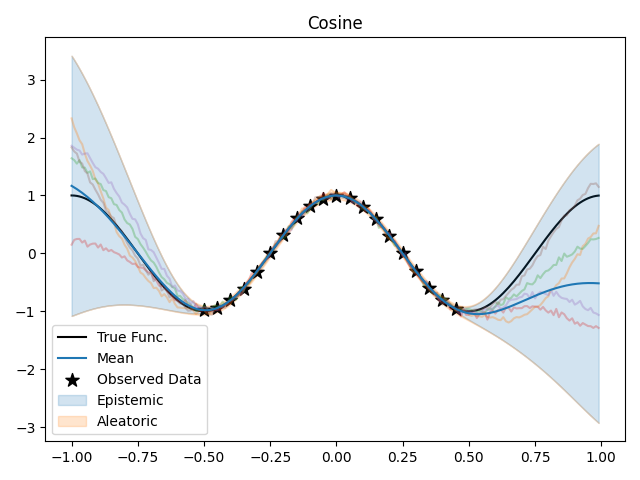
\includegraphics[width=\linewidth, height=0.618033988749895\linewidth]{graphics/generated/gp-cosine-rfsf.tikz}}
\newcommand{\imageResultsGpCosineRbf}      {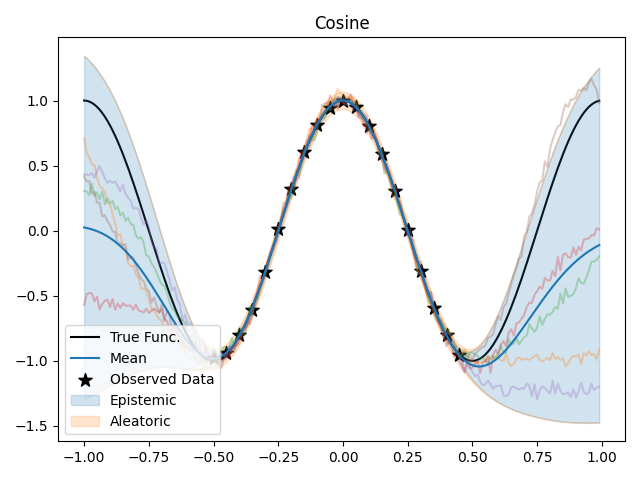
\includegraphics[width=\linewidth, height=0.618033988749895\linewidth]{graphics/generated/gp-cosine-rbf.tikz}}
\newcommand{\imageResultsGpCosineRff}      {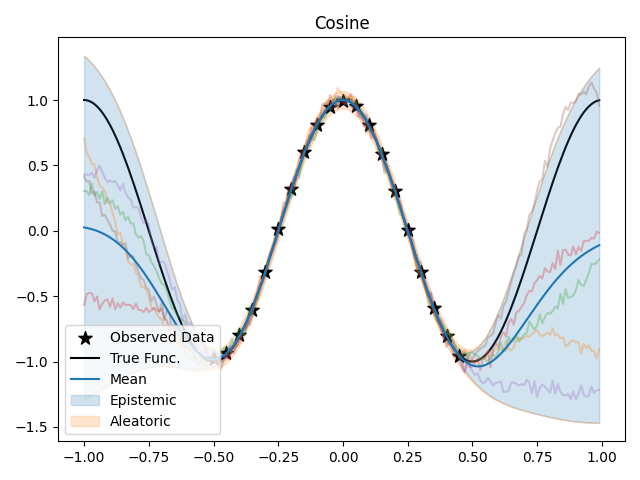
\includegraphics[width=\linewidth, height=0.618033988749895\linewidth]{graphics/generated/gp-cosine-rff.tikz}}
\newcommand{\imageResultsGpHeavisideRfsf}  {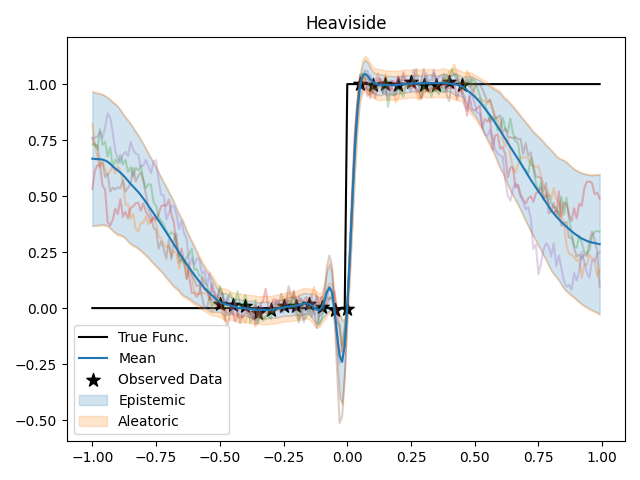
\includegraphics[width=\linewidth, height=0.618033988749895\linewidth]{graphics/generated/gp-heaviside-rfsf.tikz}}
\newcommand{\imageResultsGpHeavisideRbf}   {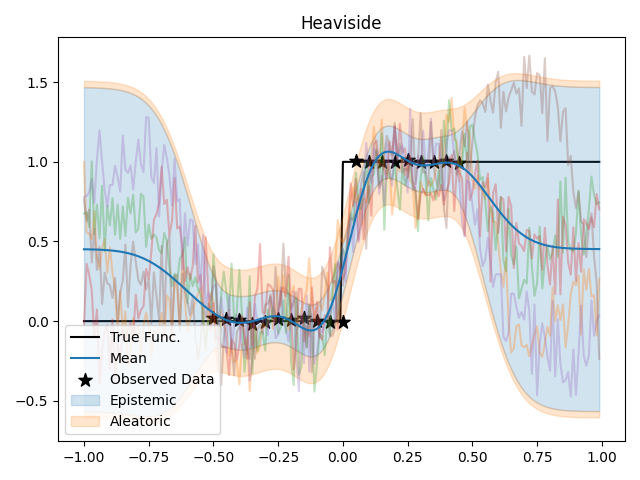
\includegraphics[width=\linewidth, height=0.618033988749895\linewidth]{graphics/generated/gp-heaviside-rbf.tikz}}
\newcommand{\imageResultsGpHeavisideRff}   {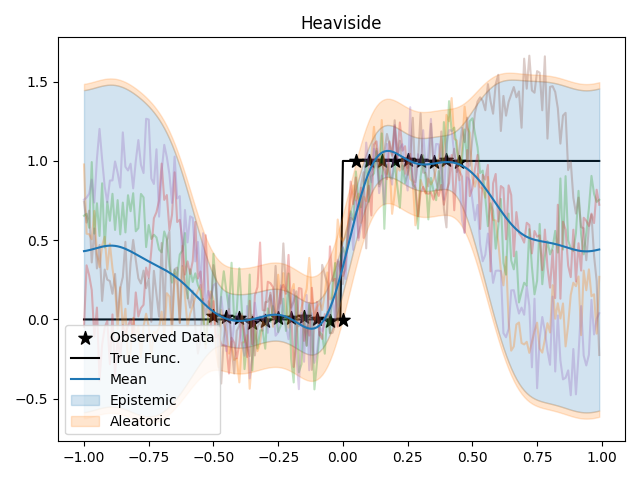
\includegraphics[width=\linewidth, height=0.618033988749895\linewidth]{graphics/generated/gp-heaviside-rff.tikz}}
\newcommand{\imageResultsGpHeavicosineRfsf}{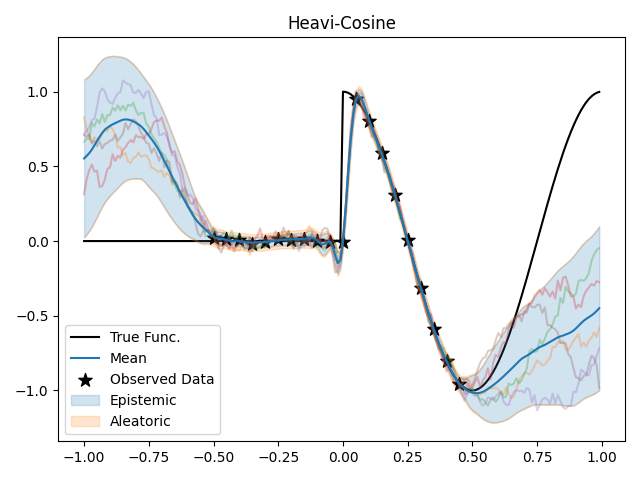
\includegraphics[width=\linewidth, height=0.618033988749895\linewidth]{graphics/generated/gp-heavicosine-rfsf.tikz}}
\newcommand{\imageResultsGpHeavicosineRbf} {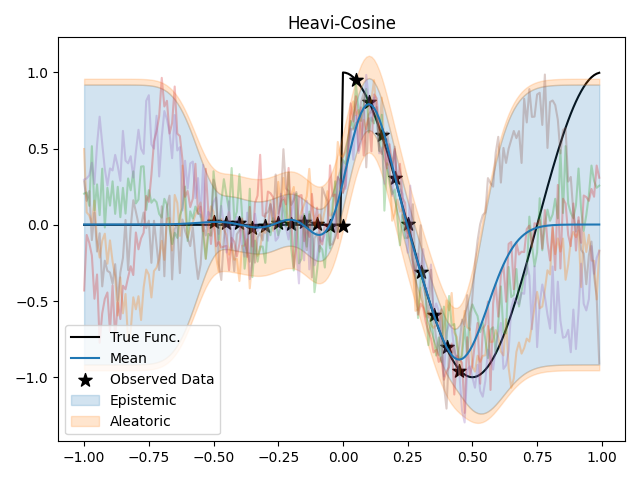
\includegraphics[width=\linewidth, height=0.618033988749895\linewidth]{graphics/generated/gp-heavicosine-rbf.tikz}}
\newcommand{\imageResultsGpHeavicosineRff} {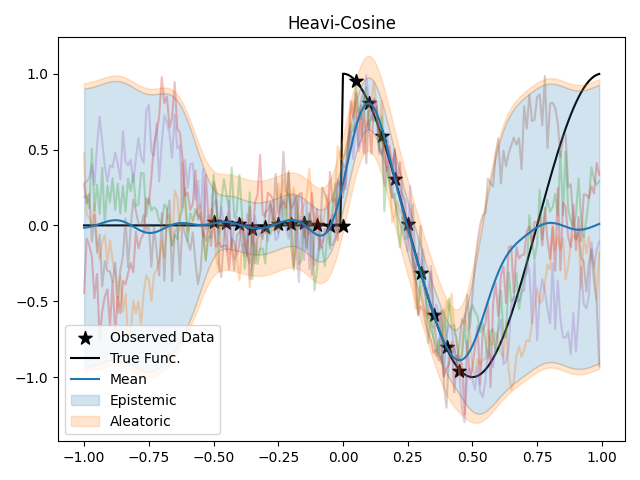
\includegraphics[width=\linewidth, height=0.618033988749895\linewidth]{graphics/generated/gp-heavicosine-rff.tikz}}
\newcommand{\imageResultsGpGapcosineRfsf}  {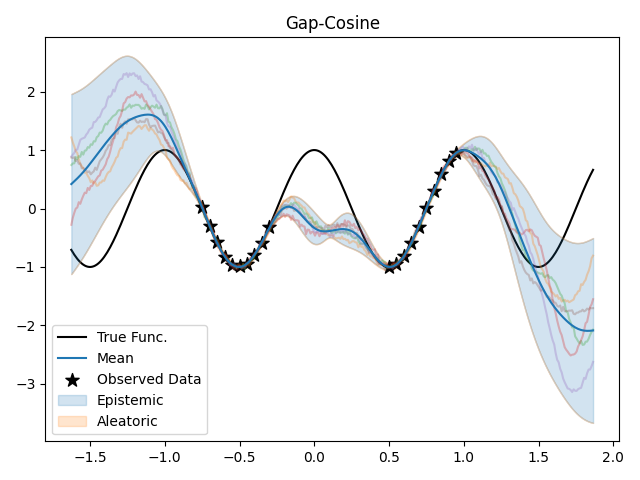
\includegraphics[width=\linewidth, height=0.618033988749895\linewidth]{graphics/generated/gp-gapcosine-rfsf.tikz}}
\newcommand{\imageResultsGpGapcosineRbf}   {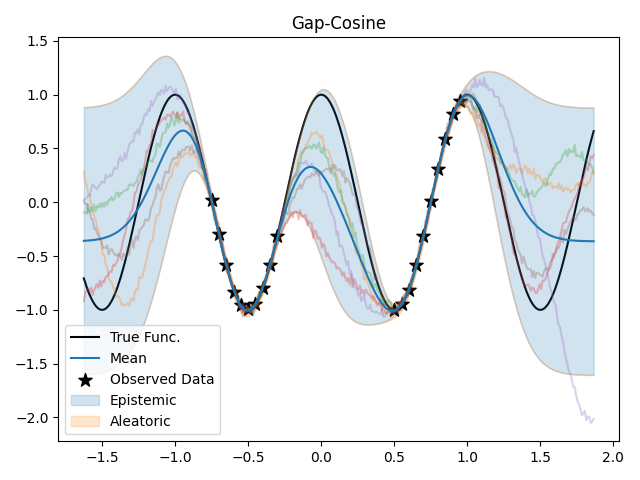
\includegraphics[width=\linewidth, height=0.618033988749895\linewidth]{graphics/generated/gp-gapcosine-rbf.tikz}}
\newcommand{\imageResultsGpGapcosineRff}   {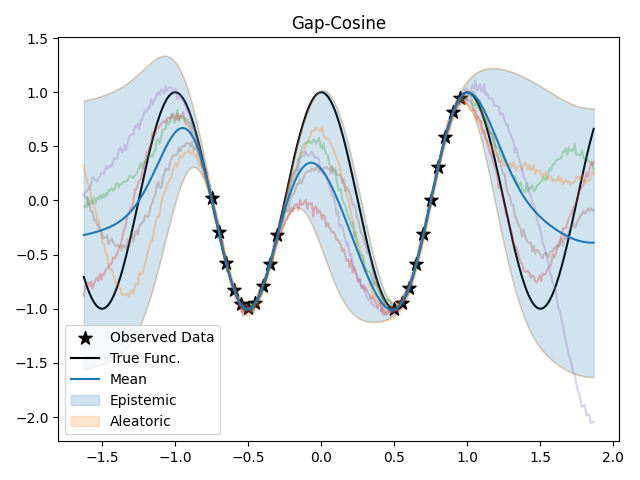
\includegraphics[width=\linewidth, height=0.618033988749895\linewidth]{graphics/generated/gp-gapcosine-rff.tikz}}


\newcommand{\tabResultsSynthetic}{
	\scriptsize
	\begin{tabular}{c|cc|ccccc}
		\toprule
		& & & \multicolumn{5}{c}{\textbf{Data Set}} \\[1pt]
		& \multicolumn{2}{c|}{\textbf{Model}}         & Cosine                 & Heaviside              & Heavi-Cosine            & Gap-Cosine             & Cartpole                          \\
		\midrule \multirow{5}{*}{\rotatebox{90}{\textbf{Log-Lik.}}}
		& \multirow[t]{3}{*}{\acs{RFSF}} & Random     & \textbf{\texttt{2.43}} & \texttt{0.11}          & \texttt{-1.66}          & \texttt{1.27}          & \texttt{~-9.88\,±\,1.86}          \\
		&                                & \acs{ReLU} & \texttt{2.34}          & \textbf{\texttt{0.80}} & \texttt{-0.90}          & \texttt{1.50}          & \texttt{-12.30\,±\,2.31}          \\
		&                                & \acs{SH}   & \texttt{2.37}          & \textbf{\texttt{0.21}} & \texttt{-1.23}          & \texttt{1.52}          & \texttt{~-9.73\,±\,2.10}          \\
		& \multirow[t]{2}{*}{\acs{GP}}   & \acs{SE}   & \textbf{\texttt{2.44}} & \texttt{0.73}          & \textbf{\texttt{~0.77}} & \textbf{\texttt{2.58}} & \textbf{\texttt{~-3.21\,±\,1.64}} \\
		&                                & \acs{RFF}  & \textbf{\texttt{2.44}} & \texttt{0.73}          & \textbf{\texttt{~0.78}} & \textbf{\texttt{2.59}} & \texttt{~-7.38\,±\,1.94}          \\
		\midrule \multirow{5}{*}{\rotatebox{90}{\textbf{\acs{RMSE}}}}
		& \multirow[t]{3}{*}{\acs{RFSF}} & Random     & \texttt{0.45}          & \texttt{0.35}          & \texttt{~0.55}          & \texttt{0.91}          & \texttt{~~0.91\,±\,0.08}          \\
		&                                & \acs{ReLU} & \textbf{\texttt{0.39}} & \texttt{1.06}          & \texttt{~3.55}          & \texttt{1.62}          & \texttt{~~1.01\,±\,0.10}          \\
		&                                & \acs{SH}   & \texttt{0.70}          & \texttt{0.35}          & \texttt{~0.48}          & \texttt{0.75}          & \texttt{~~0.98\,±\,0.11}          \\
		& \multirow[t]{2}{*}{\acs{GP}}   & \acs{SE}   & \texttt{0.45}          & \textbf{\texttt{0.30}} & \textbf{\texttt{~0.29}} & \textbf{\texttt{0.40}} & \textbf{\texttt{~~0.77\,±\,0.07}} \\
		&                                & \acs{RFF}  & \texttt{0.45}          & \textbf{\texttt{0.31}} & \textbf{\texttt{~0.30}} & \texttt{0.42}          & \texttt{~~1.26\,±\,0.10}          \\
		\bottomrule
	\end{tabular}
}

\newcommand{\tabResultsUciJoe}{
	\scriptsize
	\begin{tabular}{c|cc|cccc}
		\toprule
		& & & \multicolumn{4}{c}{\textbf{Data Set}} \\[1pt]
		& \multicolumn{2}{c|}{\textbf{Model}}                               & Boston                           & Concrete                         & Power                            & Yacht                            \\
		\midrule \multirow{11}{*}{\rotatebox{90}{\textbf{Log-Lik.}}}
		& \multirow[t]{3}{*}{\acs{RFSF}}             & Random           & \texttt{-2.40\,±\,0.05}          & \textbf{\texttt{-2.94\,±\,0.05}} & \texttt{-2.78\,±\,0.01}          & \texttt{-0.80\,±\,0.02}          \\
		&                                            & \acs{ReLU}       & \texttt{-2.39\,±\,0.05}          & \textbf{\texttt{-2.93\,±\,0.04}} & \texttt{-2.80\,±\,0.01}          & \texttt{-0.86\,±\,0.02}          \\
		&                                            & \acs{SH}         & \texttt{-2.44\,±\,0.06}          & \textbf{\texttt{-2.94\,±\,0.05}} & \texttt{-2.78\,±\,0.01}          & \texttt{-0.83\,±\,0.02}          \\
		& \multirow[t]{2}{*}{\acs{GP}}               & \acs{SE}         & \textbf{\texttt{-2.38\,±\,0.05}} & \textbf{\texttt{-2.98\,±\,0.06}} & \texttt{-2.82\,±\,0.01}          & \texttt{-0.80\,±\,0.02}          \\
		&                                            & \acs{RFF}        & \texttt{-2.40\,±\,0.06}          & \textbf{\texttt{-3.01\,±\,0.05}} & \texttt{-2.84\,±\,0.01}          & \texttt{-0.80\,±\,0.02}          \\
		& \multirow[t]{2}{*}{\acs{GBLL}}\superdagger & Leaky \acs{ReLU} & \texttt{-2.90\,±\,0.05}          & \texttt{-3.09\,±\,0.03}          & \texttt{-2.77\,±\,0.01}          & \texttt{-1.67\,±\,0.11}          \\
		&                                            & Tanh             & \texttt{-3.06\,±\,0.03}          & \texttt{-3.21\,±\,0.03}          & \texttt{-2.83\,±\,0.01}          & \texttt{-0.70\,±\,0.10}          \\
		& \multirow[t]{2}{*}{Ensemble}\superdagger   & Leaky \acs{ReLU} & \texttt{-2.48\,±\,0.09}          & \textbf{\texttt{-3.04\,±\,0.08}} & \textbf{\texttt{-2.70\,±\,0.01}} & \texttt{-0.35\,±\,0.07}          \\
		&                                            & Tanh             & \texttt{-2.48\,±\,0.08}          & \textbf{\texttt{-3.03\,±\,0.07}} & \textbf{\texttt{-2.72\,±\,0.01}} & \textbf{\texttt{-0.03\,±\,0.05}} \\
		& \multirow[t]{2}{*}{\acs{MAP}}\superdagger  & Leaky \acs{ReLU} & \texttt{-2.60\,±\,0.07}          & \texttt{-3.04\,±\,0.04}          & \texttt{-2.77\,±\,0.01}          & \texttt{-5.14\,±\,1.62}          \\
		&                                            & Tanh             & \texttt{-2.59\,±\,0.06}          & \texttt{-3.11\,±\,0.04}          & \texttt{-2.76\,±\,0.01}          & \texttt{-1.77\,±\,0.53}          \\
		\midrule \multirow{11}{*}{\rotatebox{90}{\textbf{\acs{RMSE}}}}
		& \multirow[t]{3}{*}{\acs{RFSF}}             & Random           & \textbf{\texttt{~2.95\,±\,0.15}} & \textbf{\texttt{~4.70\,±\,0.14}} & \texttt{~3.90\,±\,0.03}          & \texttt{~0.51\,±\,0.03}          \\
		&                                            & \acs{ReLU}       & \texttt{~3.51\,±\,0.44}          & \texttt{~4.77\,±\,0.15}          & \texttt{~3.95\,±\,0.04}          & \texttt{~0.53\,±\,0.03}          \\
		&                                            & \acs{SH}         & \texttt{~3.17\,±\,0.17}          & \textbf{\texttt{~4.66\,±\,0.15}} & \texttt{~3.88\,±\,0.03}          & \texttt{~0.52\,±\,0.03}          \\
		& \multirow[t]{2}{*}{\acs{GP}}               & \acs{SE}         & \textbf{\texttt{~2.81\,±\,0.12}} & \texttt{~4.98\,±\,0.15}          & \texttt{~4.03\,±\,0.03}          & \texttt{~0.51\,±\,0.04}          \\
		&                                            & \acs{RFF}        & \texttt{~2.98\,±\,0.13}          & \texttt{~5.08\,±\,0.15}          & \texttt{~4.11\,±\,0.03}          & \texttt{~0.52\,±\,0.04}          \\
		& \multirow[t]{2}{*}{\acs{GBLL}}\superdagger & Leaky \acs{ReLU} & \texttt{~4.19\,±\,0.17}          & \texttt{~5.01\,±\,0.18}          & \texttt{~3.85\,±\,0.03}          & \texttt{~1.09\,±\,0.09}          \\
		&                                            & Tanh             & \texttt{~4.61\,±\,0.23}          & \texttt{~5.50\,±\,0.23}          & \texttt{~4.09\,±\,0.04}          & \texttt{~0.43\,±\,0.03}          \\
		& \multirow[t]{2}{*}{Ensemble}\superdagger   & Leaky \acs{ReLU} & \textbf{\texttt{~2.79\,±\,0.17}} & \textbf{\texttt{~4.55\,±\,0.12}} & \textbf{\texttt{~3.59\,±\,0.04}} & \texttt{~0.83\,±\,0.08}          \\
		&                                            & Tanh             & \textbf{\texttt{~2.71\,±\,0.13}} & \textbf{\texttt{~4.51\,±\,0.13}} & \textbf{\texttt{~3.66\,±\,0.04}} & \textbf{\texttt{~0.38\,±\,0.03}} \\
		& \multirow[t]{2}{*}{\acs{MAP}}\superdagger  & Leaky \acs{ReLU} & \texttt{~3.02\,±\,0.17}          & \textbf{\texttt{~4.75\,±\,0.12}} & \texttt{~3.81\,±\,0.04}          & \texttt{~0.94\,±\,0.09}          \\
		&                                            & Tanh             & \textbf{\texttt{~3.01\,±\,0.17}} & \texttt{~5.15\,±\,0.13}          & \texttt{~3.78\,±\,0.04}          & \textbf{\texttt{~0.39\,±\,0.04}} \\
		\bottomrule
	\end{tabular}
}

\newcommand{\tabResultsUciRest}{
	\begin{tabular}{c|cc|ccccc}
		\toprule
		& & & \multicolumn{5}{c}{\textbf{Data Set}} \\[1pt]
		& \multicolumn{2}{c|}{\textbf{Model}}             & Energy                           & Kin8nm                           & Naval                                 & Protein                              & Wine                             \\
		\midrule \multirow{5}{*}{\rotatebox{90}{\textbf{Log-Lik.}}}
		& \multirow[t]{3}{*}{\acs{RFSF}} & Random         & \textbf{\texttt{-0.70\,±\,0.02}} & \texttt{~0.68\,±\,0.05}          & \texttt{~~-78.19\,±\,~69.72}          & \texttt{~~-2.94\,±\,~~0.03}          & \texttt{-0.11\,±\,0.07}          \\
		&                                & \acs{ReLU}     & \texttt{-0.74\,±\,0.02}          & \textbf{\texttt{~0.97\,±\,0.03}} & \texttt{~-172.57\,±\,104.83}          & \texttt{-629.05\,±\,384.60}          & \texttt{-0.11\,±\,0.06}          \\
		&                                & \acs{SH}       & \texttt{-0.74\,±\,0.02}          & \texttt{~0.52\,±\,0.07}          & \texttt{~~-62.69\,±\,~55.40}          & \texttt{~~-2.96\,±\,~~0.03}          & \textbf{\texttt{ 0.01\,±\,0.06}} \\
		& \multirow[t]{2}{*}{\acs{GP}}   & \acs{SE}       & \textbf{\texttt{-0.68\,±\,0.02}} & \texttt{-0.22\,±\,0.24}          & \textbf{\texttt{~~~~6.91\,±\,~~0.15}} & \textbf{\texttt{~~-2.89\,±\,~~0.00}} & \texttt{-0.84\,±\,0.05}          \\
		&                                & \acs{RFF}      & \textbf{\texttt{-0.69\,±\,0.02}} & \texttt{~0.75\,±\,0.04}          & \texttt{-1941.56\,±\,248.64}          & \texttt{~~-2.90\,±\,~~0.00}          & \texttt{-0.89\,±\,0.04}          \\
		\midrule \multirow{5}{*}{\rotatebox{90}{\textbf{\acs{RMSE}}}}
		& \multirow[t]{3}{*}{\acs{RFSF}} & Random         & \textbf{\texttt{~0.48\,±\,0.02}} & \textbf{\texttt{~0.07\,±\,0.00}} & \texttt{~~~~0.01\,±\,0.00~~}          & \textbf{\texttt{~~~3.97\,±\,0.02~~}} & \textbf{\texttt{~0.64\,±\,0.01}} \\
		&                                & \acs{ReLU}     & \textbf{\texttt{~0.49\,±\,0.02}} & \textbf{\texttt{~0.07\,±\,0.00}} & \texttt{~~~~0.01\,±\,0.00~~}          & \textbf{\texttt{~~~4.00\,±\,0.03~~}} & \texttt{~0.66\,±\,0.01}          \\
		&                                & \acs{SH}       & \textbf{\texttt{~0.49\,±\,0.02}} & \texttt{~0.08\,±\,0.00}          & \texttt{~~~~0.01\,±\,0.00~~}          & \textbf{\texttt{~~~3.97\,±\,0.02~~}} & \texttt{~0.65\,±\,0.01}          \\
		& \multirow[t]{2}{*}{\acs{GP}}   & \acs{SE}       & \textbf{\texttt{~0.48\,±\,0.02}} & \texttt{~0.08\,±\,0.00}          & \textbf{\texttt{~~~~0.00\,±\,0.00~~}} & \texttt{~~~4.34\,±\,0.01~~}          & \textbf{\texttt{~0.63\,±\,0.01}} \\
		&                                & \acs{RFF}      & \textbf{\texttt{~0.48\,±\,0.01}} & \textbf{\texttt{~0.07\,±\,0.00}} & \texttt{~~~~0.02\,±\,0.00~~}          & \texttt{~~~4.42\,±\,0.01~~}          & \textbf{\texttt{~0.63\,±\,0.01}} \\
		\bottomrule
	\end{tabular}
}


% This is not allowed in the poster as the poster uses biblatex.
\usepackage[nobreak]{cite}

\begin{document}
    \title{Random Fourier Series Features}
    \author{
        \IEEEauthorblockN{Fabian~Damken}
        \IEEEauthorblockA{fabian.damken@stud.tu-darmstadt.de}
        \and
        \IEEEauthorblockN{Joe~Watson}
        \IEEEauthorblockA{joe.watson@tu-darmstadt.de}
        \and
        \IEEEauthorblockN{Jan~Peters}
        \IEEEauthorblockA{jan.peters@tu-darmstadt.de}
    }
    \date{\today}

    \maketitle

    \begin{abstract}
        \lipsum{1}

    \end{abstract}
	\acresetall

    \section{Introduction}
    (Deep) \acp{NN} are extremely powerful and expressive machine learning models dominating the current landscape of artificial intelligence\cite{krizhevskyImageNetClassificationDeep2012}.
While they have great predictive power, \acp{NN} usually lack uncertainty estimation and a Bayesian treatment.
In Bayesian machine learning, we not only seek models that predict some value, but that also gauge their uncertainty about the prediction.
While frequentistic models are capable of estimating aleatoric (i.e., noise-induced) uncertainty, Bayesian models include epistemic uncertainty that quantifies the model's trust "in itself."
Quantification of the uncertainty is useful in a variety of domains such as \ac{MPC}\cite{hewingLearningBasedModelPredictive2020,bradfordStochasticDatadrivenModel2020}.

\begin{figure}
	\centering
	\includegraphics[width=\linewidth]{graphics/hypercube.tikz}
	\caption{
		Connections between various (Bayesian) regression models.
		The three axis distinct them between using kernels vs. features (blue), relying on manually designing vs. learning (yellow), and stationary vs. non-stationary behavior (green).
		\acsp{RFSF} (our method) are not clearly stationary or non-stationary and theoretical analysis is up to future research.
		Abbreviations used in the figure: \acs{SE} (Squared Exponential), \acs{RFF} (Random Fourier Features), \acs{RFSF} (Random Fourier Series Features), \acs{NLM} (Neural Linear Model), \acs{NTK} (Neural Tangent Kernel), \acs{DKL} (Deep Kernel Learning)
	}
	\label{fig:hypercube}
\end{figure}

A proposed class of extensions for \acp{NN} are \acp{BNN}\cite{mackayPracticalBayesianFramework1992,nealBayesianLearningNeural2012} combining the expressiveness of \acp{NN} with uncertainty quantification.
However, exact inference is intractable, so these methods have to resort to approximate inference approaches\cite{nealBayesianLearningNeural2012,hernandez-lobatoProbabilisticBackpropagationScalable2015,denkerTransformingNeuralNetOutput1990,galDropoutBayesianApproximation2016,lakshminarayananSimpleScalablePredictive2017,blundellWeightUncertaintyNeural2015}.
Also, \acp{BNN} suffer from various drawbacks such as expensive and complicated training, inaccurate posteriors, and unreliable uncertainty quantification\cite{foongExpressivenessApproximateInference2020,foongInBetweenUncertaintyBayesian2019,osbandRandomizedPriorFunctions2018,ovadiaCanYouTrust2019,wenzelHowGoodBayes2020,yaoQualityUncertaintyQuantification2019}.
Hence, they are not suitable for application in high-stakes domains such as medical diagnosis where accurate uncertainty quantification is necessary\cite{watsonLatentDerivativeBayesian2021}.

A well-known alternative approach for Bayesian machine learning are \acp{GP}.
\aclp{GP} allow exact inference leveraging linear regression.
Using a kernel for lifting the inputs into a high-, and possibly infinite-, dimensional feature space allows great flexibility.
Despite the great uncertainty estimation of \acp{GP}, their raw prediction power is limited by and highly dependent on the kernel.
This dependence is reflected in the amount of kernels that have been studied throughout the years\cite[ch.\,2]{duvenaudAutomaticModelConstruction2014}.
Motivated by this limitation, methods for (deep) kernel learning (\acsu{DKL}) have been developed\cite{wilsonDeepKernelLearning2016,calandraManifoldGaussianProcesses2016,jacotNeuralTangentKernel2020}.
However, exact inference with kernels is a tedious task requiring inversion of an \(N \times N\)-matrix (the Gram matrix) where \(N\) is the number of data points.
The computational complexity of this is cubic, prohibiting online use of \acp{GP} for large data sets\cite{rahimiRandomFeaturesLargeScale2007}.
Approaches for reducing the computational complexity have been proposed such as inducing points\cite{snelsonSparseGaussianProcesses2005} or the Nyström method\cite{nystromUberPraktischeAuflosung1930,sunReviewNystromMethods2015}.

Alternatively, one can resort to Bayesian linear regression with features.
To mimic \ac{GP} regression, these features are chosen to approximate a kernel, e.g., the \ac{SE} kernel.
A well-known choice are \acp{RFF} that can approximate arbitrary stationary kernels and are often configured for the \ac{SE} kernel as this is possible in closed form\cite{rahimiRandomFeaturesLargeScale2007}.
However, the \ac{SE} kernel usually produces results that are too smooth\cite{steinInterpolationSpatialData1999} and is, by design, not able to capture functions with non-stationary length-scale.

\emph{Contribution:} We propose an extension of \acp{RFF}, \acp{RFSF}, that build a bridge between (a) \acp{RFF}, (b) \ac{DKL}, and (c) \acp{BNN} by (a) reducing the computational complexity of \ac{GP} regression due to working with features, (b) enrich the capacity of \acp{GP} by adding more parameters and reducing the need of (manually) designed kernels, and (c) using classical training methods known from \acp{NN} for optimizing the hyper-parameters.
\Cref{fig:hypercube} illustrates these connections on three axis: kernels vs. features, designing vs. learning, and stationary vs. non-stationary length-scales.
Despite the lack of a proof and given only empirical evidence, we found that \acp{RFSF} can represent various kernels and features, bridging the gap between stationary and non-stationary kernels.

We will now highlight connections to related work (\cref{sec:relatedWork}).
Subsequently, we will lay out some preliminaries (\cref{sec:preliminaries}), present the methodology of \acp{RFSF} in \cref{sec:methods}, and finally empirically evaluate and summarize our findings as well as provide direction for future research (\cref{sec:eval,sec:conclusion}).


    \section{Related Work}  \label{sec:relatedWork}
    We closely follow\cite{watsonLatentDerivativeBayesian2021} here.
We structure related work into the origins of motivation for this work: \aclp{BNN} and \aclp{GP}.

\paragraph{Bayesian Neural Networks}
\acl{BNN} have a long history directly using \acp{NN} as statistical models\cite{mackayPracticalBayesianFramework1992} and for regularization\cite{hintonKeepingNeuralNetworks1993}.
Many approaches are based on \ac{MCMC}\cite{andrieuIntroductionMCMCMachine2003,hoffmanNoUTurnSamplerAdaptively2014,chenStochasticGradientHamiltonian2014}, however, these approaches are computationally expensive and scale poorly with larger models.
This motivated the development of \ac{VI} methods\cite{hintonKeepingNeuralNetworks1993,petersonExplorationsMeanField1989,gravesPracticalVariationalInference2011}.
Some alternative approximation techniques are, for instance, Laplace approximation\cite{mackayPracticalBayesianFramework1992,denkerTransformingNeuralNetOutput1990,ritterScalableLaplaceApproximation2018}, ensembles\cite{lakshminarayananSimpleScalablePredictive2017,osbandRandomizedPriorFunctions2018,barberEnsembleLearningBayesian1998,pearceUncertaintyNeuralNetworks2020}, and expectation propagation\cite{hernandez-lobatoProbabilisticBackpropagationScalable2015}.
Another alternative are \acp{BLL} networks where the last layer-weights are treated in a Bayesian fashion\cite{lazaro-gredillaMarginalizedNeuralNetwork2010}.
They have successfully been applied in a variety of tasks\cite{snoekScalableBayesianOptimization2015,weberOptimizingBayesianLast2018,riquelmeDeepBayesianBandits2018,pinslerBayesianBatchActive2019,odonoghueUncertaintyBellmanEquation2018,oberBenchmarkingNeuralLinear2019}.


\paragraph{Gaussian Processes}
It was shown that \acp{NN} with infinite width are equivalent to \acp{GP} under mild conditions\cite{nealBayesianLearningNeural2012}.
But also beyond this equivalence a lot of focus is put on the intersection of \acp{GP} and \acp{BNN}.
\ac{DKL}\cite{wilsonDeepKernelLearning2016} is concerned with learning closed-form deep kernels using \acp{NN} to find more expressive covariance functions.
A similar idea are manifold \acp{GP}\cite{calandraManifoldGaussianProcesses2016} which extract intermediate features from data on which a designed covariance function performs better.
Despite the great success of \acp{GP}, exact inference is computationally expensive.
This motivated the development of approximate \acp{GP} in many fashions such as inducing points and direct approximations of the kernel\cite{nystromUberPraktischeAuflosung1930,rahimiRandomFeaturesLargeScale2007}.


    \section{Preliminaries}  \label{sec:preliminaries}
    \subsection{Fourier Series}
	\emph{Fourier series} are a principled way to represent any periodic function (satisfying the Dirichlet conditions\cite{oppenheimSignalsSystems1997}) as a linear combination of sine and cosine waves.
	The resulting approximation $\hat{f}_K$ of the function $f$ can be represented in three different fashions: in sine-cosine form, amplitude-phase form, and exponential form.
	In the sine-cosine form, the series is represented by the sum of separate sine and cosine waves with separate amplitudes,
	\begin{equation}
		\hat{f}_K(x) = \frac{a_0}{2} + \sum_{k = 1}^{K} a_k \cos(\pi k x / \tilde{T}) + b_k \sin(\pi k x / \tilde{T}),
		\label{eq:sineCosineFourierSeries}
	\end{equation}
	where the Fourier coefficients $a_k$ and $b_k$ are given by
	\begin{align}
		a_k &= \frac{1}{\tilde{T}} \int_{x_0}^{x_0 + 2\tilde{T}} f(x) \cos(\pi k x / \tilde{T}) \dd{x} \\
		b_k &= \frac{1}{\tilde{T}} \int_{x_0}^{x_0 + 2\tilde{T}} f(x) \sin(\pi k x / \tilde{T}) \dd{x}.
	\end{align}
	Here, $\tilde{T}$ is half the period of $f$ (for instance, $f(x) = \sin(x)$ has the half-period $\tilde{T} = \pi$).
	In amplitude-phase form,
	\begin{equation}
		\hat{f}_K(x) = \frac{A_0}{2} + \sum_{k = 1}^{K} A_k \cos(2 \pi k x / \tilde{T} - \varphi_k),
	\end{equation}
	the series is represented by individual cosine waves with amplitudes and phases.
	These can be computed from the Fourier coefficients as follows:
	\begin{align}
		A_k &= \sqrt{a_k^2 + b_k^2} &
		\varphi_k &= \mathrm{arctan2}(b_k, a_k).
	\end{align}
	For the following, we stick to the former version (sine-cosine) for practical reasons:
	the amplitude-phase formulation introduces some ambiguity as $\varphi \equiv \varphi + 2\pi$.
	When optimizing numerically, this can cause problems due to either having ambiguous optima or having to include constraints.
% end

\subsection{Gaussian Process Regression}
%	In supervised learning, we are concerned with modeling a function $f : \mathcal{X} \to \mathcal{Y}$ from input data $\mathcal{X}$ to labels $\mathcal{Y}$ using an (approximate) model $\hat{f} : \mathcal{X} \to \mathcal{Y}$.
%	The model is trained on a labeled dataset $\mathcal{D} = \{ (\vec{x}_i, y_i) \}_{i = 1, \dots, N} \subseteq \mathcal{X} \times \mathcal{Y}$.
%	For regression, the target labels $\mathcal{Y}$ are continuous: $\mathcal{Y} \subseteq \R$.
%	Various methods exist for tackling this problem, e.g., linear regression, \acp{SVM}, and \acp{NN}.
%	Bayesian methods take this idea one step further and not only model the mapping from inputs to targets but also quantify their epistemic uncertainty.
%	This idea can be incorporated into linear regression, for example, by placing a prior on the feature weights and computing the posterior of new data given the training data.
%	Gauging the (epistemic) uncertainty is helpful in various domains such as robust \ac{MPC}.
%	Incorporating uncertainty allows the controller to vary its trust in the underlying model, avoiding unknown and potentially unsafe terrain.

	\ac{GP} regression can be viewed in two fashions:
	firstly, as an extension of linear regression to an infinite number of features.
	This involves computing the limit $n \to \infty$ where $n$ is the number of features.
	Secondly, as an infinite Gaussian distribution over a function space where every finite subset of the random variables is jointly Gaussian.
	However, both definitions (or views) yield the exact same result.
	For the rest of this report we will stick to the former definition.

	We closely follow\cite{rasmussenGaussianProcessesMachine2006} in terms of notation, refer to them for a more thorough treatment of \ac{GP} regression and its derivation, and will give a brief overview over the used notation.
	Let \(\vec{x}_\ast\) and \(y_\ast\) be a test input and target\footnote{When predicting, the target is not known and the \ac{GP} defines a Gaussian distribution over it.}, respectively, then the \ac{GP} regression posterior is a Gaussian distribution with the following mean and variance:
	\begin{equation}
		\begin{aligned}
			\E[y_\ast] &= \vec{k}_\ast^\transposed \mat{K}^{-1} \vec{y} &
			\V[y_\ast] &= k_\ast - \vec{k}_\ast^\transposed \mat{K}^{-1} \vec{k}_\ast
		\end{aligned}
		\label{eq:gp}
	\end{equation}
	Here, \( \mat{K} \) denotes the Gram matrix on the training inputs, \(\vec{k}_\ast\) denotes the evaluation of the kernel between the test input and train inputs organized into a column vector, and \(k_\ast\) is the kernel evaluation of the test input \(\vec{x}_\ast\); train targets are organized into \(\vec{y}\).

	An exemplary kernel is the \ac{SE} kernel \( k_\mathrm{SE}(\vec{x} - \vec{y}) = \exp{ -\lVert \vec{x} - \vec{y} \rVert_2^2 / (2 \ell^2) } \) with the length-scale\footnote{The length-scale determines the "roughness" of the function samples\cite[p.\,15]{rasmussenGaussianProcessesMachine2006}.} \(\ell^2\).
	However, it has been shown that this kernel often exhibits extremely smooth functions (as it is infinitely differentiable) often unrealistic for real-world data\cite{steinInterpolationSpatialData1999}.
	% TODO: When at the ULB before submitting this thing: search specific page in Stein's book.
	Despite its drawbacks, the \ac{SE} kernel remains one of the most widely used kernels due to its simplicity and applicability\cite[p.\,83]{rasmussenGaussianProcessesMachine2006}.

	While employing the "kernel trick" allows great flexibility with (potentially) infinite-dimensional feature spaces, it introduces major computational challenges due to the inversion of the Gram matrix in \cref{eq:gp}.
	That is, the inversion has time complexity \( \mathcal{O}(N^3) \), where \(N\) is the number of data points in the training data set.
%	One approach for tackling this problem are \acl{RFF} that resort to Bayesian regression by choosing appropriate features that approximate a desired kernel.
	One approach for tackling this problem are \acl{RFF}.
% end


    \section{Methods}  \label{sec:methods}
    %	- random Fourier features in a more formal way
%	- highlight extension done by random Fourier _series_ features
%	- maybe do a bit of theoretical elaboration
%	- describe process of finding the hyper-parameters (empirical Bayes)
%	- transition to empirical evaluation

\subsection{Random Fourier Features}
By explicitly modeling the features, the inversion of the Gram matrix can be avoided by resorting to computing the distribution over the weights explicitly.
A well-known approach for this are \acp{RFF}\cite{rahimiRandomFeaturesLargeScale2007} which approximate the \ac{SE} kernel.
A single \ac{RFF} is given by
\begin{equation}
    \vec{z}_{\vec{\omega}}(\vec{x}) =
        \begin{bmatrix}
            \cos(\vec{\omega} \dotproduct \vec{x}) \\
            \sin(\vec{\omega} \dotproduct \vec{x})
        \end{bmatrix}\!.
    \label{eq:rffFeature}
\end{equation}
This definition is based on the observation that
\begin{equation}
    k(\vec{x} - \vec{y}) = \E_{\vec{\omega} \sim p(\cdot)}\bigl[ \vec{z}_{\vec{\omega}}(\vec{x}) \dotproduct \vec{z}_{\vec{\omega}}(\vec{y}) \bigr]
    \label{eq:rffExpectation}
\end{equation}
where $k(\vec{x} - \vec{y})$ is a stationary kernel and $p(\vec{\omega})$ is its Fourier transform (which is a proper probability distribution due to Bochner's theorem\cite{steinInterpolationSpatialData1999}).
For the \ac{SE} kernel, $p(\omega)$ is tractable and is equal to a standard normal distribution\cite{rasmussenGaussianProcessesMachine2006}.
As the integral \eqref{eq:rffExpectation} is intractable, it is usually approximated using Monte-Carlo estimation over $\vec{\omega}$ (another methods for evaluation the integral are, for example, quadrature methods\cite{daoGaussianQuadratureKernel2017}).
Let ${\vec{w}_j}_{j = 1}^{D}$ be the particles sampled from $p(\vec{\omega})$.
The corresponding feature particles, $\vec{z}_{\vec{\omega}_j}(\cdot)$ are then concatenated, forming the complete feature $\vec{z}(\cdot)$ which is scaled by $1/\sqrt{D}$ such that the inner product yields the usual Monte Carlo approximation of an expectation.


\subsection{Random Fourier Series Features}
We extend \acp{RFF} to Random Fourier \emph{Series} Features (\acsu{RFSF}) by splitting up \eqref{eq:rffFeature} further into sub-features with separate amplitudes for the sine/cosine component and adding the respective scaling factors for $\vec{x}$:
\begin{equation}
    \tilde{\vec{z}}_{\vec{\omega}}^{\,(k)}(\vec{x}) =
        \begin{bmatrix}
            a_k \cos(\pi k \mel{\vec{\omega}}{\mat{\Lambda}^{-1}}{\vec{x}} / \tilde{T}) \\
            b_k \sin(\pi k \mel{\vec{\omega}}{\mat{\Lambda}^{-1}}{\vec{x}} / \tilde{T})
        \end{bmatrix}\!.
\end{equation}
which are then summed over $k = 1, 2, \dots, M$.
The matrix $\mat{\Lambda}$ represents the length-scales which can be either isotropic for a single length-scale but also different for the input dimensions, leading to \ac{ARD}.
This formulation is inspired by the sine-cosine formulation of a Fourier series \eqref{eq:sineCosineFourierSeries}, motivating the name.
Note that the half-period $\tilde{T}$ has the function of a "secondary" length-scale and applied equally to all input dimensions.

To find the optimal hyper-parameters $\vec{a}_{0:M}$, $\vec{b}_{0:M}$, and $\mat{\Lambda}$, we use the empirical Bayes approximation\cite[p.\,165]{bishopPatternRecognitionMachine2006}, i.e., maximize the marginal log-likelihood over the training data.
As will be seen in the evaluation section, the result is highly dependent on the half-period $\tilde{T}$, hence it will be treated as an additional hyper-parameter.  \todo{did we see this in evaluation?}
Beyond the kernel's parameters, the data is assumed to have Gaussian aleatoric noise with zero mean and variance $\sigma_n^2$ which is again an additional hyper-parameter.














%\begin{comment}
\begin{figure*}
\begin{align}
    \tilde{k}(\vec{x}, \vec{y})
        &= \ip{\tilde{\vec{z}}_{\vec{\omega}}(\vec{x})}{\tilde{\vec{z}}_{\vec{\omega}}(\vec{y})} \\
        &= \ip{\sum_{m = 1}^{M} \tilde{\vec{z}}_{\vec{\omega}}^{\,(m)}(\vec{x})}{\sum_{m = 1}^{M} \tilde{\vec{z}}_{\vec{\omega}}^{\,(m)}(\vec{y})} \\
        &= \ip{\sum_{m = 1}^{M}  \begin{bmatrix} a_m \cos(x_m) \\ b_m \sin(x_m) \end{bmatrix}}{\sum_{m = 1}^{M} \begin{bmatrix} a_m \cos(y_m) \\ b_m \sin(y_m) \end{bmatrix}} \\
        &= \ip{\begin{bmatrix} \sum_{m = 1}^{M} a_m \cos(x_m) \\ \sum_{m = 1}^{M} b_m \sin(x_m) \end{bmatrix}}{\begin{bmatrix} \sum_{m = 1}^{M} a_m \cos(y_m) \\ \sum_{m = 1}^{M} b_m \sin(y_m) \end{bmatrix}} \\
        &= \Biggl(\, \sum_{m = 1}^{M} a_m \cos(x_m) \Biggr) \Biggl(\, \sum_{m = 1}^{M} a_m \cos(y_m) \Biggr) + \Biggl(\, \sum_{m = 1}^{M} b_m \sin(x_m) \Biggr) \Biggl(\, \sum_{m = 1}^{M} b_m \sin(y_m) \Biggr) \\
        &= \sum_{m = 1}^{M} \sum_{n = 1}^{M} a_m a_n \cos(x_m) \cos(y_n) + \sum_{m = 1}^{M} \sum_{n = 1}^{M} b_m b_n \sin(x_m) \sin(y_n) \\
        &= \sum_{m = 1}^{M} \sum_{n = 1}^{M} a_m a_n \cos(x_m) \cos(y_n) + b_m b_n \sin(x_m) \sin(y_n) \\
        &= \frac{1}{2} \sum_{m = 1}^{M} \sum_{n = 1}^{M} (a_m a_n + b_m b_n) \cos(x_m - y_n) + (a_m a_n - b_m b_n) \cos(x_m + y_n) \\
\end{align}

\begin{align}
    \E_{\vec{\omega}}\Bigl[ \tilde{k}(\vec{x}, \vec{y}) \Bigr]
        &= \frac{1}{2} \sum_{m = 1}^{M} \sum_{n = 1}^{M} (a_m a_n + b_m b_n) \E_{\vec{\omega}}\bigl[ \cos(x_m - y_n) \bigr] + (a_m a_n - b_m b_n) \E_{\vec{\omega}}\bigl[ \cos(x_m + y_n) \bigr] \\
        &= \frac{1}{2} \sum_{m = 1}^{M} \sum_{n = 1}^{M} (a_m a_n + b_m b_n) \, k_\mathrm{SE}\bigl( m \vec{x} - n \vec{y}; \pi^{-1} \tilde{T} \ell^2 \bigr) + (a_m a_n - b_m b_n) \, k_\mathrm{SE}\bigl( m \vec{x} - (-n \vec{y}); \pi^{-1} \tilde{T} \ell^2 \bigr) \\
\end{align}

\begin{equation}
    \E_{\vec{\omega}}\bigl[ \cos(x_m - y_n) \bigr]
        = \E_{\vec{\omega}}\biggl[ \cos\biggl( \frac{\pi}{\tilde{T} \ell^2} \ip{\vec{\omega}}{m \vec{x} - n \vec{y}} \biggr) \biggr]
        = k_\mathrm{SE}\bigl( m \vec{x} - n \vec{y}; \pi^{-1} \tilde{T} \ell^2 \bigr)
\end{equation}
\begin{equation}
    \E_{\vec{\omega}}\bigl[ \cos(x_m + y_n) \bigr]
        = k_\mathrm{SE}\bigl( m \vec{x} - (-n \vec{y}); \pi^{-1} \tilde{T} \ell^2 \bigr)
\end{equation}

\begin{align}
    x_m \pm y_n &= \frac{\pi}{\tilde{T} \ell^2} \ip{\vec{\omega}}{m \vec{x} \pm n \vec{y}}
\end{align}

    \caption{Some derivations that are likely to not make sense.}
\end{figure*}
%\end{comment}


    \section{Evaluation}  \label{sec:eval}
    In this section, we will empirically evaluate the proposed \acp{RFSF}.
We aim to assess the following central hypotheses:
\begin{hypothesis}
	"Do \acp{RFSF} outperform \acp{RFF} (due to their increased parameter capacity)?"
	\label{hyp:rfsfAreBetter}
\end{hypothesis}
Additionally, we try to answer:
\begin{hypothesis}
	How do different initial values of the feature's amplitudes affect the performance?
	\label{hyp:initialValues}
\end{hypothesis}
In the following, we will first present some implementation details (\cref{subsec:impl}) and subsequently present the experiment setup (\cref{subsec:setup}) and results (\cref{subsec:results}).


\subsection{Implementation}  \label{subsec:impl}
	We implemented \acp{RFSF} using GPyTorch\cite{jacotNeuralTangentKernel2020} and used Adam\cite{kingmaAdamMethodStochastic2017a} for maximizing the marginal log-likelihood.
	Despite the computational advantage of not having to compute (and, most importantly, invert) the Gram matrix, we implemented \acp{RFSF} directly as a GPyTorch kernel.
	This allows a unified view and evaluation when comparing to well-known kernels like the \ac{SE} kernel.
	Also, it allowed to just modifying the existing implementation of \acp{RFF}, reducing the risk of mistakes.
	We published our implementation on \href{https://github.com/fdamken/random-fourier-series-features}{GitHub}\footnote{\url{https://github.com/fdamken/random-fourier-series-features}}.
% end


\subsection{Experiment Setup}  \label{subsec:setup}
	To assess our hypothesis, we evaluate our approach on three classes of data sets: synthetic (\cref{tab:dataSynthetic}), \ac{UCI}\cite{duaUCIMachineLearning2017} (\cref{tab:dataUci}), and robotics (real data from a cartpole with the states as inputs and control signal as target).
	The model quality is measured by the \ac{RMSE} and log-likelihood on the test data (using the test/train splits provided along\cite{galDropoutBayesianApproximation2016} for a fair comparison).
	While the \ac{RMSE} on the mean measures raw predictive performance and how closely the mean follows the true data, the log-likelihood also assess the uncertainty quantification.
	For \ac{RFSF}, we assess three different initializations of the amplitudes:
	\begin{itemize}
		\item \emph{Random:}               Sampled from a uniform distribution, i.e., $\vec{a}_{0:M}, \vec{b}_{0:M} \sim \mathcal{U}(0, 1)$.
		\item \emph{\ac{ReLU}:}            Taken from the Fourier series for a periodic \ac{ReLU}, i.e., $a_m = (\tilde{T} (-1)^m - \tilde{T}) / (m^2 \pi^2)$ and $b_m = -(\tilde{T} (-1)^m) / (m \pi)$ for $m > 0$ and $a_0 = \tilde{T}/2$ and $b_0 = 0$ (see \cref{app:perelu} for further details and the derivation).
		\item \emph{\acl{SH} (\acsu{SH}):} All set to zero except for the $0$-th which are set to one, i.e., $a_0 = b_0 = 1$, $\vec{a}_{1:M} = \vec{b}_{1:M} = \vec{0}$.
	\end{itemize}
	The idea behind each is as follows.
	The random initialization is most simplistic and a baseline for the others.
	Initializing the amplitudes as (periodic) \acp{ReLU} sets the connection to kernel learning and \acp{BNN} with the \ac{ReLU} being one of the most common activation functions.
	Starting with a single harmonic similar to \acp{RFF} connects \acp{RFSF} closer to the idea behind \acp{RFF} and serves as an assessment of our hypothesis that \acp{RFSF} should have higher capacity than \acp{RFF} (i.e., if the marginal log-likelihood would not get better by touching the other amplitudes, they shall not change).

	We compare our method to the \ac{SE} and \ac{RFF} kernels.
	For some data sets (\ac{UCI} Boston, Concrete, Power, and Yacht), we also compare to popular approaches for \acp{BNN}:
	\begin{itemize}
		\item \emph{Gaussian Bayesian Last Layer (\acsu{GBLL})\cite{rasmussenGaussianProcessesMachine2006}:}
			A \ac{BLL} \ac{NN} with Gaussian conjugate prior on the weight.
%			With $\vec{\phi}_{\vec{\theta}}(\vec{x})$ being the parameterized features induced by the \ac{NN} and $\mat{\Lambda}_0$ being the covariance of the prior, this is equivalent to a \ac{GP} with kernel $k_{\vec{\theta}}(\vec{x}, \vec{y}) = \vec{\phi}_{\vec{\theta}}(\vec{x})^\transposed \mat{\Lambda}_0^{-1} \vec{\phi}_{\vec{\theta}}(\vec{y})$.
		\item \emph{Ensemble\cite{lakshminarayananSimpleScalablePredictive2017}:}
			An ensemble of \acp{NN} all of which provide mean and variance of the target.
			Using some neat tricks during training, Ensemble provides predictions along with uncertainty quantification.
		\item \emph{Maximum A-Posteriori (\acsu{MAP}):}
			Regularized neural network trained to output mean and covariance of the target.
	\end{itemize}
	We include results for this models for a broader comparison, however, we did not implement them ourselves and took the results from\cite{watsonLatentDerivativeBayesian2021} (with permission).

	\begin{table}
		\centering
		\begin{tabular}{lll}
			\toprule
			\textbf{Name}         & \textbf{Function}         & \textbf{Domain}                   \\ \midrule
			Cosine                & $\cos(2 \pi x)$           & $[-0.5, 0.5]$                     \\
			Heaviside\superdagger & $\Theta(x)$               & $[-0.5, 0.5]$                     \\
			Heavi-Cosine          & $\Theta(x) \cos(2 \pi x)$ & $[-0.5, 0.5]$                     \\
			Gap-Cosine            & $\cos(2 \pi x)$           & $[-0.75, -0.25) \cup (0.5, 0.75]$ \\ \bottomrule
		\end{tabular}
		\caption{
			Synthetic Data Sets;
			All data sets are augmented with additive zero-mean Gaussian noise with $\sigma^2 = \num{e-4}$.
			\superdagger{}The heaviside function is defined as $ \Theta(x) = \max\{ 0, \mathrm{sign}(x) \} $
		}
		\label{tab:dataSynthetic}
	\end{table}

	\begin{table}
		\centering
		\begin{tabular}{lll}
			\toprule
			\textbf{Name}                 & \textbf{Short Name} & \textbf{Source}\cite{duaUCIMachineLearning2017}                  \\ \midrule
			Boston Housing                & Boston              &                                                                  \\
			Concrete Compression Strength & Concrete            & \cite{yehModelingStrengthHighperformance1998}                    \\
			Combined Cycle Power Plant    & Power               & \cite{kayaLocalGlobalLearning2012,tufekciPredictionFullLoad2014} \\
			Yacht                         & Yacht               &                                                                  \\
			Energy Efficiency             & Energy              & \cite{tsanasAccurateQuantitativeEstimation2012}                  \\
			Kinematics of 8-Link Robot    & Kin8nm              &                                                                  \\
			Naval Propulsion Plants       & Naval               & \cite{coradduMachineLearningApproaches2016}                      \\
			Protein Tertiary Structure    & Protein             &                                                                  \\
			Wine Quality (Red)            & Wine                & \cite{cortezModelingWinePreferences2009}                         \\ \bottomrule
		\end{tabular}
		\caption{\acs{UCI} Data Sets}
		\label{tab:dataUci}
	\end{table}
% end

\subsection{Results}  \label{subsec:results}
	We first compare visually the quality of \acp{RFSF} to the \ac{SE} kernel (and \acp{RFF}) on the synthetic data.
	As this data is one-dimensional, it is straightforward to visualize.
	\Cref{fig:syntheticResultPlot} (on \cpageref{fig:syntheticResultPlot}) shows the results of the aforementioned kernels on the synthetic data.
	It can be seen that the \acp{RFF} are hardly distinguishable from \ac{SE} (which makes sense as \acp{RFF} can be proven to approximate the \ac{SE} kernel).
	Therefore, we only discuss differences between \acp{RFSF} and the \ac{SE} kernel which can be transferred to comparing \acp{RFSF} to \acp{RFF}.
	For every data set except the Gap-Cosine, both \acp{RFSF} and the \ac{SE} kernel approximate the true function reasonably, although \ac{SE} fails to capture discontinuities (Heaviside and Heavi-Cosine) and makes them extremely smooth.
	However, both kernels exhibit a small length-scale not appropriate for the functions.
	This is visible in the roughness of the \ac{GP} samples and is especially prevailing for the \ac{SE} on the Heaviside and Heavi-Cosine data sets (\cref{fig:syntheticResultPlotSeHeaviside,fig:syntheticResultPlotSeHeaviCosine}).
	This shows that \acp{RFSF} can capture non-stationary trends (cf. \cref{fig:hypercube}) opposed to the \ac{SE} kernel.
	For the Gap-Cosine data set, the \ac{SE} kernel (\cref{fig:syntheticResultPlotSeGapCosine}) clearly outperforms \acp{RFSF} (\cref{fig:syntheticResultPlotRfsfGapCosine}) within the gap by actually capturing the overall trend (with the true function lying withing the confidence interval).

	Quantitative results for all data sets are summarized in \cref{tab:results}.
	\Cref{tab:resultsSynthetic} contains results for the synthetic data (and Cartpole) and \cref{tab:resultsUciJoe} contains \ac{UCI}-results and, for a broader comparison, some results from\cite{watsonLatentDerivativeBayesian2021}.
	The results for the remaining \ac{UCI} data sets not covered in \cref{tab:resultsUciJoe} are given in \cref{tab:resultsUciRest} in appendix \cref{app:remainingResults} for brevity (the results on the reduced data sets is sufficient for the discussion).

	\subsubsection{Synthetic Data Sets}
		On synthetic data, \acp{RFSF} perform roughly equal to the \ac{SE} kernel and \acp{RFF} on the Cosine data set in terms of the log-likelihood and outperform both in terms of the \ac{RMSE} (again on the Cosine data set).
		Also, they perform better on the Heaviside data set in terms of the log-likelihood.
		However, for all other metrics (log-likelihood and \ac{RMSE} of Heavi-Cosine and Gap-Cosine as well as \ac{RMSE} on Heaviside), either the \ac{SE} kernel or \acp{RFF} outperform all variants of \acp{RFSF}.

		Focusing just on the \acp{RFSF} variants, no clear trend can be determined in terms of the log-likelihood.
		For the \ac{RMSE}, however, the \ac{ReLU} initialization is (with the exception of Cosine) outperformed by one of the other variants (Random or \ac{SH}).
	% end

	\subsubsection{\acs{UCI} Data Sets}
		In terms of the log-likelihood, \acp{RFSF} are either outperformed by or equal to the \ac{SE} kernel and Ensemble.
		For the remaining data sets in \cref{tab:resultsUciRest} for which\cite{watsonLatentDerivativeBayesian2021} do not report results, the results are similar.
		Within the class of \acp{RFSF} variants, the Random initialization is often superior w.r.t. to log-likelihood and \ac{RMSE}.
	% end

	\subsubsection{Cartpole Data Set}
		On the Cartpole data set, the \ac{SE} kernel outperforms \acp{RFSF} and \acp{RFF} in both log-likelihood and \ac{RMSE} by far.
		For the different \acp{RFSF} variants, no clear distinction (difference of more than the measurement uncertainty) is visible.
	% end

	\begin{figure*}
		\centering
%		\begin{subfigure}{0.32\linewidth}
%			\centering
%			\imageResultsGpCosineRfsf
%			\caption{\acsp{RFSF} on Cosine}
%		\end{subfigure}
%		~
%		\begin{subfigure}{0.32\linewidth}
%			\centering
%			\imageResultsGpCosineRbf
%			\caption{\acs{SE} on Cosine}
%		\end{subfigure}
%		~
%		\begin{subfigure}{0.32\linewidth}
%			\centering
%			\imageResultsGpCosineRff
%			\caption{\acsp{RFF} on Cosine}
%		\end{subfigure}
%		\\[0.4cm]
		\begin{subfigure}{0.32\linewidth}
			\centering
			\imageResultsGpHeavisideRfsf
			\caption{\acsp{RFSF} on Heaviside}
		\end{subfigure}
		~
		\begin{subfigure}{0.32\linewidth}
			\centering
			\imageResultsGpHeavisideRbf
			\caption{\acs{SE} on Heaviside}
			\label{fig:syntheticResultPlotSeHeaviside}
		\end{subfigure}
		~
		\begin{subfigure}{0.32\linewidth}
			\centering
			\imageResultsGpHeavisideRff
			\caption{\acsp{RFF} on Heaviside}
		\end{subfigure}
		\\[0.4cm]
		\begin{subfigure}{0.32\linewidth}
			\centering
			\imageResultsGpHeavicosineRfsf
			\caption{\acsp{RFSF} on Heavi-Cosine}
		\end{subfigure}
		~
		\begin{subfigure}{0.32\linewidth}
			\centering
			\imageResultsGpHeavicosineRbf
			\caption{\acs{SE} on Heavi-Cosine}
			\label{fig:syntheticResultPlotSeHeaviCosine}
		\end{subfigure}
		~
		\begin{subfigure}{0.32\linewidth}
			\centering
			\imageResultsGpHeavicosineRff
			\caption{\acsp{RFF} on Heavi-Cosine}
		\end{subfigure}
		\\[0.4cm]
		\begin{subfigure}{0.32\linewidth}
			\centering
			\imageResultsGpGapcosineRfsf
			\caption{\acsp{RFSF} on Gap-Cosine}
			\label{fig:syntheticResultPlotRfsfGapCosine}
		\end{subfigure}
		~
		\begin{subfigure}{0.32\linewidth}
			\centering
			\imageResultsGpGapcosineRbf
			\caption{\acs{SE} on Gap-Cosine}
			\label{fig:syntheticResultPlotSeGapCosine}
		\end{subfigure}
		~
		\begin{subfigure}{0.32\linewidth}
			\centering
			\imageResultsGpGapcosineRff
			\caption{\acsp{RFF} on Gap-Cosine}
		\end{subfigure}
		\caption{
			\acl{GP} regression results using \acsp{RFSF}, \acsp{SE}, and \acsp{RFF} kernels for the synthetic data sets.
			The shaded areas depict the epistemic/aleatoric (posterior) uncertainty, the blue solid line depicts the (posterior) mean, the black stars are the training samples, and the black solid line depicts the true function.
			The colorful lines are samples from the \acsp{GP}.
%			Axis labels and ticks where left out for brevity as the results are purely qualitative and specific numbers do not matter.
		}
		\label{fig:syntheticResultPlot}
	\end{figure*}

	\begin{table*}
		\centering
		\begin{subtable}{\linewidth}
			\centering
			\tabResultsSynthetic
			\caption{Results for the synthetic and robotics data sets.}
			\label{tab:resultsSynthetic}
		\end{subtable}
		\\[0.5cm]
		\begin{subtable}{\linewidth}
			\centering
			\tabResultsUciJoe
			\caption{
				Results for the \acs{UCI} datasets.
				\superdagger{}Values taken from\cite{watsonLatentDerivativeBayesian2021} with permission.
			}
			\label{tab:resultsUciJoe}
		\end{subtable}
		\caption{
			Evaluation results for the presented data sets.
			For UCI and Cartpole, the mean along with the measurement uncertainty are computed over the provided train/test splits.
			The synthetic data sets only have a single train/test split, hence no uncertainty can be provided.
			Both the log-likelihood and \acs{RMSE} are reported where the higher and lower values are better, respectively.
			The best values for a data set are depicted boldface.
			Values are considered equal if their confidence regions overlap (w.r.t. the best mean value).
			The results for the remaining data sets are given in \cref{tab:resultsUciRest} in \cref{app:remainingResults}.
		}
		\label{tab:results}
	\end{table*}
% end


    \section{Conclusion}  \label{sec:conclusion}
    \lipsum{1}


    \FloatBarrier
    \bibliographystyle{IEEEtran}
    \bibliography{IEEEabrv,literature}
    \FloatBarrier


	\appendix

	\subsection{Fourier Series of the Periodic \acs{ReLU}}  \label{app:perelu}
	Using the ReLU, we define the \emph{Periodic} \ac{ReLU} (\acsu{PeReLU}) $\PeReLU(x) \coloneqq \ReLU\bigl([x + \tilde{T}]_{2\tilde{T}} - \tilde{T}\bigr)$, where $[\cdot]_U$ is the modulus operator w.r.t. $U$ defined as $[\cdot]_U : \R \to \R^+ : u \mapsto \min\bigl\{ u + zU \,:\, u + zU \geq 0,\, z \in \Z \bigr\}$.
The $\pm \tilde{T}$ in the \ac{PeReLU} definition ensures that the \ac{PeReLU} still has the usual \ac{ReLU} properties in a region around zero, i.e., that $\PeReLU(x) = 0$ for $x < 0$ and $\PeReLU(x) = x$ for $x > 0$.
The coefficients of the Fourier series $a_m$ and $b_m$ for $m > 0$ are then given as
\begin{align}
    a_m &= \frac{1}{\tilde{T}} \int_{-\tilde{T}}^{\tilde{T}}\! \PeReLU(x) \cos(m \pi x / \tilde{T}) \dd{x} \\
        &= \frac{1}{\tilde{T}} \int_{-\tilde{T}}^{\tilde{T}}\! \ReLU(x) \cos(m \pi x / \tilde{T}) \dd{x} \\
        &= \frac{1}{\tilde{T}} \int_{0}^{\tilde{T}}\! x \cos(m \pi x / \tilde{T}) \dd{x} \\
        %&= \frac{1}{m \pi} \bigl[ x \sin(m \pi x / \tilde{T}) \bigr]_{x \,=\, 0}^{x \,=\,\tilde{T}} - \frac{1}{m \pi} \int_0^{\tilde{T}}\! \sin(m \pi x / \tilde{T}) \dd{x} \\
        %&= \frac{1}{m \pi} \bigl[ x \sin(m \pi x / \tilde{T}) \bigr]_{x \,=\, 0}^{x \,=\,\tilde{T}} + \frac{\tilde{T}}{m^2\pi^2} \bigl[ \cos(m \pi x / \tilde{T}) \bigr]_{x \,=\, 0}^{x \,=\,\tilde{T}} \\
        %&= \frac{\tilde{T}}{m \pi} \sin(m \pi) + \frac{\tilde{T}}{m^2\pi^2} \cos(m \pi) - \frac{\tilde{T}}{m^2\pi^2} \\
        %&= \frac{\tilde{T} (-1)^m }{m^2\pi^2} - \frac{\tilde{T}}{m^2\pi^2} \\
        &= \frac{\tilde{T} (-1)^m - \tilde{T}}{m^2\pi^2} \\
    b_m &= \frac{1}{\tilde{T}} \int_{-\tilde{T}}^{\tilde{T}}\! \PeReLU(x) \sin(m \pi x / \tilde{T}) \dd{x} \\
        &= \frac{1}{\tilde{T}} \int_{-\tilde{T}}^{\tilde{T}}\! \ReLU(x) \sin(m \pi x / \tilde{T}) \dd{x} \\
        &= \frac{1}{\tilde{T}} \int_{0}^{\tilde{T}}\! x \sin(m \pi x / \tilde{T}) \dd{x} \\
        %&= -\frac{1}{m \pi} \bigl[ x \cos(m \pi x / \tilde{T}) \bigr]_{x \,=\, 0}^{x \,=\,\tilde{T}} + \frac{1}{m \pi} \int_0^{\tilde{T}}\! \cos(m \pi x / \tilde{T}) \dd{x} \\
        %&= -\frac{1}{m \pi} \bigl[ x \cos(m \pi x / \tilde{T}) \bigr]_{x \,=\, 0}^{x \,=\,\tilde{T}} + \frac{\tilde{T}}{m^2\pi^2} \bigl[ \sin(m \pi x / \tilde{T}) \bigr]_{x \,=\, 0}^{x \,=\,\tilde{T}} \\
        %&= -\frac{\tilde{T}}{m \pi} \cos(m \pi) + \frac{\tilde{T}}{m^2\pi^2} \sin(m \pi) \\
        &= -\frac{\tilde{T} (-1)^m}{m \pi}
\end{align}
where the remaining integrals can be solved by partial integration.
For $m = 0$, the coefficients are simply $a_0 = \tilde{T}/2$ and $b_0 = 0$.


	\subsection{Influence of the Half-Period}  \label{app:halfPeriodInfluence}
	We noticed a major influence of the half-period during hyper-parameter optimization using Optuna\cite{akibaOptunaNextgenerationHyperparameter2019}.
That is, the higher the (initial) value of \(\tilde{T}\), the higher the objective (see \cref{fig:optunaParallelCoordinates}).
As a consequence we included the half-period into the set of (hyper-) parameter that are optimized using empirical Bayes, however, this phenomenon is still in place.
This is also reflected in Optuna's importance rating of \num{0.86}.

\begin{figure}
	\centering
	\resizebox{\linewidth}{!}{%% Creator: Matplotlib, PGF backend
%%
%% To include the figure in your LaTeX document, write
%%   \input{<filename>.pgf}
%%
%% Make sure the required packages are loaded in your preamble
%%   \usepackage{pgf}
%%
%% Also ensure that all the required font packages are loaded; for instance,
%% the lmodern package is sometimes necessary when using math font.
%%   \usepackage{lmodern}
%%
%% Figures using additional raster images can only be included by \input if
%% they are in the same directory as the main LaTeX file. For loading figures
%% from other directories you can use the `import` package
%%   \usepackage{import}
%%
%% and then include the figures with
%%   \import{<path to file>}{<filename>.pgf}
%%
%% Matplotlib used the following preamble
%%   \usepackage{fontspec}
%%   \setmainfont{DejaVuSerif.ttf}[Path=\detokenize{/home/fdamken/Development/study/random-fourier-series-features/venv/lib/python3.8/site-packages/matplotlib/mpl-data/fonts/ttf/}]
%%   \setsansfont{DejaVuSans.ttf}[Path=\detokenize{/home/fdamken/Development/study/random-fourier-series-features/venv/lib/python3.8/site-packages/matplotlib/mpl-data/fonts/ttf/}]
%%   \setmonofont{DejaVuSansMono.ttf}[Path=\detokenize{/home/fdamken/Development/study/random-fourier-series-features/venv/lib/python3.8/site-packages/matplotlib/mpl-data/fonts/ttf/}]
%%
\begingroup%
\makeatletter%
\begin{pgfpicture}%
\pgfpathrectangle{\pgfpointorigin}{\pgfqpoint{6.400000in}{4.800000in}}%
\pgfusepath{use as bounding box, clip}%
\begin{pgfscope}%
\pgfsetbuttcap%
\pgfsetmiterjoin%
\definecolor{currentfill}{rgb}{1.000000,1.000000,1.000000}%
\pgfsetfillcolor{currentfill}%
\pgfsetlinewidth{0.000000pt}%
\definecolor{currentstroke}{rgb}{1.000000,1.000000,1.000000}%
\pgfsetstrokecolor{currentstroke}%
\pgfsetdash{}{0pt}%
\pgfpathmoveto{\pgfqpoint{0.000000in}{0.000000in}}%
\pgfpathlineto{\pgfqpoint{6.400000in}{0.000000in}}%
\pgfpathlineto{\pgfqpoint{6.400000in}{4.800000in}}%
\pgfpathlineto{\pgfqpoint{0.000000in}{4.800000in}}%
\pgfpathlineto{\pgfqpoint{0.000000in}{0.000000in}}%
\pgfpathclose%
\pgfusepath{fill}%
\end{pgfscope}%
\begin{pgfscope}%
\pgfsetbuttcap%
\pgfsetmiterjoin%
\definecolor{currentfill}{rgb}{1.000000,1.000000,1.000000}%
\pgfsetfillcolor{currentfill}%
\pgfsetlinewidth{0.000000pt}%
\definecolor{currentstroke}{rgb}{0.000000,0.000000,0.000000}%
\pgfsetstrokecolor{currentstroke}%
\pgfsetstrokeopacity{0.000000}%
\pgfsetdash{}{0pt}%
\pgfpathmoveto{\pgfqpoint{0.800000in}{0.528000in}}%
\pgfpathlineto{\pgfqpoint{2.784000in}{0.528000in}}%
\pgfpathlineto{\pgfqpoint{2.784000in}{4.224000in}}%
\pgfpathlineto{\pgfqpoint{0.800000in}{4.224000in}}%
\pgfpathlineto{\pgfqpoint{0.800000in}{0.528000in}}%
\pgfpathclose%
\pgfusepath{fill}%
\end{pgfscope}%
\begin{pgfscope}%
\definecolor{textcolor}{rgb}{0.000000,0.000000,0.000000}%
\pgfsetstrokecolor{textcolor}%
\pgfsetfillcolor{textcolor}%
\pgftext[x=0.800000in,y=0.389111in,,top]{\color{textcolor}\sffamily\fontsize{10.000000}{12.000000}\selectfont Objective}%
\end{pgfscope}%
\begin{pgfscope}%
\pgfsetbuttcap%
\pgfsetroundjoin%
\definecolor{currentfill}{rgb}{0.000000,0.000000,0.000000}%
\pgfsetfillcolor{currentfill}%
\pgfsetlinewidth{0.803000pt}%
\definecolor{currentstroke}{rgb}{0.000000,0.000000,0.000000}%
\pgfsetstrokecolor{currentstroke}%
\pgfsetdash{}{0pt}%
\pgfsys@defobject{currentmarker}{\pgfqpoint{-0.048611in}{0.000000in}}{\pgfqpoint{-0.000000in}{0.000000in}}{%
\pgfpathmoveto{\pgfqpoint{-0.000000in}{0.000000in}}%
\pgfpathlineto{\pgfqpoint{-0.048611in}{0.000000in}}%
\pgfusepath{stroke,fill}%
}%
\begin{pgfscope}%
\pgfsys@transformshift{0.800000in}{0.528000in}%
\pgfsys@useobject{currentmarker}{}%
\end{pgfscope}%
\end{pgfscope}%
\begin{pgfscope}%
\definecolor{textcolor}{rgb}{0.000000,0.000000,0.000000}%
\pgfsetstrokecolor{textcolor}%
\pgfsetfillcolor{textcolor}%
\pgftext[x=0.431782in, y=0.475238in, left, base]{\color{textcolor}\sffamily\fontsize{10.000000}{12.000000}\selectfont -8.0}%
\end{pgfscope}%
\begin{pgfscope}%
\pgfsetbuttcap%
\pgfsetroundjoin%
\definecolor{currentfill}{rgb}{0.000000,0.000000,0.000000}%
\pgfsetfillcolor{currentfill}%
\pgfsetlinewidth{0.803000pt}%
\definecolor{currentstroke}{rgb}{0.000000,0.000000,0.000000}%
\pgfsetstrokecolor{currentstroke}%
\pgfsetdash{}{0pt}%
\pgfsys@defobject{currentmarker}{\pgfqpoint{-0.048611in}{0.000000in}}{\pgfqpoint{-0.000000in}{0.000000in}}{%
\pgfpathmoveto{\pgfqpoint{-0.000000in}{0.000000in}}%
\pgfpathlineto{\pgfqpoint{-0.048611in}{0.000000in}}%
\pgfusepath{stroke,fill}%
}%
\begin{pgfscope}%
\pgfsys@transformshift{0.800000in}{1.433935in}%
\pgfsys@useobject{currentmarker}{}%
\end{pgfscope}%
\end{pgfscope}%
\begin{pgfscope}%
\definecolor{textcolor}{rgb}{0.000000,0.000000,0.000000}%
\pgfsetstrokecolor{textcolor}%
\pgfsetfillcolor{textcolor}%
\pgftext[x=0.431782in, y=1.381174in, left, base]{\color{textcolor}\sffamily\fontsize{10.000000}{12.000000}\selectfont -6.7}%
\end{pgfscope}%
\begin{pgfscope}%
\pgfsetbuttcap%
\pgfsetroundjoin%
\definecolor{currentfill}{rgb}{0.000000,0.000000,0.000000}%
\pgfsetfillcolor{currentfill}%
\pgfsetlinewidth{0.803000pt}%
\definecolor{currentstroke}{rgb}{0.000000,0.000000,0.000000}%
\pgfsetstrokecolor{currentstroke}%
\pgfsetdash{}{0pt}%
\pgfsys@defobject{currentmarker}{\pgfqpoint{-0.048611in}{0.000000in}}{\pgfqpoint{-0.000000in}{0.000000in}}{%
\pgfpathmoveto{\pgfqpoint{-0.000000in}{0.000000in}}%
\pgfpathlineto{\pgfqpoint{-0.048611in}{0.000000in}}%
\pgfusepath{stroke,fill}%
}%
\begin{pgfscope}%
\pgfsys@transformshift{0.800000in}{2.339871in}%
\pgfsys@useobject{currentmarker}{}%
\end{pgfscope}%
\end{pgfscope}%
\begin{pgfscope}%
\definecolor{textcolor}{rgb}{0.000000,0.000000,0.000000}%
\pgfsetstrokecolor{textcolor}%
\pgfsetfillcolor{textcolor}%
\pgftext[x=0.431782in, y=2.287109in, left, base]{\color{textcolor}\sffamily\fontsize{10.000000}{12.000000}\selectfont -5.4}%
\end{pgfscope}%
\begin{pgfscope}%
\pgfsetbuttcap%
\pgfsetroundjoin%
\definecolor{currentfill}{rgb}{0.000000,0.000000,0.000000}%
\pgfsetfillcolor{currentfill}%
\pgfsetlinewidth{0.803000pt}%
\definecolor{currentstroke}{rgb}{0.000000,0.000000,0.000000}%
\pgfsetstrokecolor{currentstroke}%
\pgfsetdash{}{0pt}%
\pgfsys@defobject{currentmarker}{\pgfqpoint{-0.048611in}{0.000000in}}{\pgfqpoint{-0.000000in}{0.000000in}}{%
\pgfpathmoveto{\pgfqpoint{-0.000000in}{0.000000in}}%
\pgfpathlineto{\pgfqpoint{-0.048611in}{0.000000in}}%
\pgfusepath{stroke,fill}%
}%
\begin{pgfscope}%
\pgfsys@transformshift{0.800000in}{3.245806in}%
\pgfsys@useobject{currentmarker}{}%
\end{pgfscope}%
\end{pgfscope}%
\begin{pgfscope}%
\definecolor{textcolor}{rgb}{0.000000,0.000000,0.000000}%
\pgfsetstrokecolor{textcolor}%
\pgfsetfillcolor{textcolor}%
\pgftext[x=0.431782in, y=3.193045in, left, base]{\color{textcolor}\sffamily\fontsize{10.000000}{12.000000}\selectfont -4.1}%
\end{pgfscope}%
\begin{pgfscope}%
\pgfsetbuttcap%
\pgfsetroundjoin%
\definecolor{currentfill}{rgb}{0.000000,0.000000,0.000000}%
\pgfsetfillcolor{currentfill}%
\pgfsetlinewidth{0.803000pt}%
\definecolor{currentstroke}{rgb}{0.000000,0.000000,0.000000}%
\pgfsetstrokecolor{currentstroke}%
\pgfsetdash{}{0pt}%
\pgfsys@defobject{currentmarker}{\pgfqpoint{-0.048611in}{0.000000in}}{\pgfqpoint{-0.000000in}{0.000000in}}{%
\pgfpathmoveto{\pgfqpoint{-0.000000in}{0.000000in}}%
\pgfpathlineto{\pgfqpoint{-0.048611in}{0.000000in}}%
\pgfusepath{stroke,fill}%
}%
\begin{pgfscope}%
\pgfsys@transformshift{0.800000in}{4.151742in}%
\pgfsys@useobject{currentmarker}{}%
\end{pgfscope}%
\end{pgfscope}%
\begin{pgfscope}%
\definecolor{textcolor}{rgb}{0.000000,0.000000,0.000000}%
\pgfsetstrokecolor{textcolor}%
\pgfsetfillcolor{textcolor}%
\pgftext[x=0.431782in, y=4.098980in, left, base]{\color{textcolor}\sffamily\fontsize{10.000000}{12.000000}\selectfont -2.8}%
\end{pgfscope}%
\begin{pgfscope}%
\pgfpathrectangle{\pgfqpoint{0.800000in}{0.528000in}}{\pgfqpoint{1.984000in}{3.696000in}}%
\pgfusepath{clip}%
\pgfsetrectcap%
\pgfsetroundjoin%
\pgfsetlinewidth{1.505625pt}%
\definecolor{currentstroke}{rgb}{0.925490,0.827451,0.772549}%
\pgfsetstrokecolor{currentstroke}%
\pgfsetdash{}{0pt}%
\pgfpathmoveto{\pgfqpoint{0.800000in}{2.616598in}}%
\pgfpathlineto{\pgfqpoint{2.784000in}{3.253433in}}%
\pgfusepath{stroke}%
\end{pgfscope}%
\begin{pgfscope}%
\pgfpathrectangle{\pgfqpoint{0.800000in}{0.528000in}}{\pgfqpoint{1.984000in}{3.696000in}}%
\pgfusepath{clip}%
\pgfsetrectcap%
\pgfsetroundjoin%
\pgfsetlinewidth{1.505625pt}%
\definecolor{currentstroke}{rgb}{0.670588,0.784314,0.992157}%
\pgfsetstrokecolor{currentstroke}%
\pgfsetdash{}{0pt}%
\pgfpathmoveto{\pgfqpoint{0.800000in}{1.782261in}}%
\pgfpathlineto{\pgfqpoint{2.784000in}{0.920011in}}%
\pgfusepath{stroke}%
\end{pgfscope}%
\begin{pgfscope}%
\pgfpathrectangle{\pgfqpoint{0.800000in}{0.528000in}}{\pgfqpoint{1.984000in}{3.696000in}}%
\pgfusepath{clip}%
\pgfsetrectcap%
\pgfsetroundjoin%
\pgfsetlinewidth{1.505625pt}%
\definecolor{currentstroke}{rgb}{0.752941,0.831373,0.960784}%
\pgfsetstrokecolor{currentstroke}%
\pgfsetdash{}{0pt}%
\pgfpathmoveto{\pgfqpoint{0.800000in}{2.006435in}}%
\pgfpathlineto{\pgfqpoint{2.784000in}{1.498286in}}%
\pgfusepath{stroke}%
\end{pgfscope}%
\begin{pgfscope}%
\pgfpathrectangle{\pgfqpoint{0.800000in}{0.528000in}}{\pgfqpoint{1.984000in}{3.696000in}}%
\pgfusepath{clip}%
\pgfsetrectcap%
\pgfsetroundjoin%
\pgfsetlinewidth{1.505625pt}%
\definecolor{currentstroke}{rgb}{0.890196,0.419608,0.329412}%
\pgfsetstrokecolor{currentstroke}%
\pgfsetdash{}{0pt}%
\pgfpathmoveto{\pgfqpoint{0.800000in}{3.688717in}}%
\pgfpathlineto{\pgfqpoint{2.784000in}{4.090802in}}%
\pgfusepath{stroke}%
\end{pgfscope}%
\begin{pgfscope}%
\pgfpathrectangle{\pgfqpoint{0.800000in}{0.528000in}}{\pgfqpoint{1.984000in}{3.696000in}}%
\pgfusepath{clip}%
\pgfsetrectcap%
\pgfsetroundjoin%
\pgfsetlinewidth{1.505625pt}%
\definecolor{currentstroke}{rgb}{0.909804,0.462745,0.360784}%
\pgfsetstrokecolor{currentstroke}%
\pgfsetdash{}{0pt}%
\pgfpathmoveto{\pgfqpoint{0.800000in}{3.596135in}}%
\pgfpathlineto{\pgfqpoint{2.784000in}{2.846373in}}%
\pgfusepath{stroke}%
\end{pgfscope}%
\begin{pgfscope}%
\pgfpathrectangle{\pgfqpoint{0.800000in}{0.528000in}}{\pgfqpoint{1.984000in}{3.696000in}}%
\pgfusepath{clip}%
\pgfsetrectcap%
\pgfsetroundjoin%
\pgfsetlinewidth{1.505625pt}%
\definecolor{currentstroke}{rgb}{0.913725,0.478431,0.372549}%
\pgfsetstrokecolor{currentstroke}%
\pgfsetdash{}{0pt}%
\pgfpathmoveto{\pgfqpoint{0.800000in}{3.565156in}}%
\pgfpathlineto{\pgfqpoint{2.784000in}{2.686693in}}%
\pgfusepath{stroke}%
\end{pgfscope}%
\begin{pgfscope}%
\pgfpathrectangle{\pgfqpoint{0.800000in}{0.528000in}}{\pgfqpoint{1.984000in}{3.696000in}}%
\pgfusepath{clip}%
\pgfsetrectcap%
\pgfsetroundjoin%
\pgfsetlinewidth{1.505625pt}%
\definecolor{currentstroke}{rgb}{0.866667,0.372549,0.294118}%
\pgfsetstrokecolor{currentstroke}%
\pgfsetdash{}{0pt}%
\pgfpathmoveto{\pgfqpoint{0.800000in}{3.767123in}}%
\pgfpathlineto{\pgfqpoint{2.784000in}{2.431200in}}%
\pgfusepath{stroke}%
\end{pgfscope}%
\begin{pgfscope}%
\pgfpathrectangle{\pgfqpoint{0.800000in}{0.528000in}}{\pgfqpoint{1.984000in}{3.696000in}}%
\pgfusepath{clip}%
\pgfsetrectcap%
\pgfsetroundjoin%
\pgfsetlinewidth{1.505625pt}%
\definecolor{currentstroke}{rgb}{0.925490,0.827451,0.772549}%
\pgfsetstrokecolor{currentstroke}%
\pgfsetdash{}{0pt}%
\pgfpathmoveto{\pgfqpoint{0.800000in}{2.609950in}}%
\pgfpathlineto{\pgfqpoint{2.784000in}{1.871978in}}%
\pgfusepath{stroke}%
\end{pgfscope}%
\begin{pgfscope}%
\pgfpathrectangle{\pgfqpoint{0.800000in}{0.528000in}}{\pgfqpoint{1.984000in}{3.696000in}}%
\pgfusepath{clip}%
\pgfsetrectcap%
\pgfsetroundjoin%
\pgfsetlinewidth{1.505625pt}%
\definecolor{currentstroke}{rgb}{0.772549,0.200000,0.203922}%
\pgfsetstrokecolor{currentstroke}%
\pgfsetdash{}{0pt}%
\pgfpathmoveto{\pgfqpoint{0.800000in}{4.046181in}}%
\pgfpathlineto{\pgfqpoint{2.784000in}{3.638419in}}%
\pgfusepath{stroke}%
\end{pgfscope}%
\begin{pgfscope}%
\pgfpathrectangle{\pgfqpoint{0.800000in}{0.528000in}}{\pgfqpoint{1.984000in}{3.696000in}}%
\pgfusepath{clip}%
\pgfsetrectcap%
\pgfsetroundjoin%
\pgfsetlinewidth{1.505625pt}%
\definecolor{currentstroke}{rgb}{0.913725,0.470588,0.364706}%
\pgfsetstrokecolor{currentstroke}%
\pgfsetdash{}{0pt}%
\pgfpathmoveto{\pgfqpoint{0.800000in}{3.577076in}}%
\pgfpathlineto{\pgfqpoint{2.784000in}{2.128990in}}%
\pgfusepath{stroke}%
\end{pgfscope}%
\begin{pgfscope}%
\pgfpathrectangle{\pgfqpoint{0.800000in}{0.528000in}}{\pgfqpoint{1.984000in}{3.696000in}}%
\pgfusepath{clip}%
\pgfsetrectcap%
\pgfsetroundjoin%
\pgfsetlinewidth{1.505625pt}%
\definecolor{currentstroke}{rgb}{0.933333,0.525490,0.411765}%
\pgfsetstrokecolor{currentstroke}%
\pgfsetdash{}{0pt}%
\pgfpathmoveto{\pgfqpoint{0.800000in}{3.461267in}}%
\pgfpathlineto{\pgfqpoint{2.784000in}{4.146414in}}%
\pgfusepath{stroke}%
\end{pgfscope}%
\begin{pgfscope}%
\pgfpathrectangle{\pgfqpoint{0.800000in}{0.528000in}}{\pgfqpoint{1.984000in}{3.696000in}}%
\pgfusepath{clip}%
\pgfsetrectcap%
\pgfsetroundjoin%
\pgfsetlinewidth{1.505625pt}%
\definecolor{currentstroke}{rgb}{0.815686,0.278431,0.239216}%
\pgfsetstrokecolor{currentstroke}%
\pgfsetdash{}{0pt}%
\pgfpathmoveto{\pgfqpoint{0.800000in}{3.928163in}}%
\pgfpathlineto{\pgfqpoint{2.784000in}{3.417772in}}%
\pgfusepath{stroke}%
\end{pgfscope}%
\begin{pgfscope}%
\pgfpathrectangle{\pgfqpoint{0.800000in}{0.528000in}}{\pgfqpoint{1.984000in}{3.696000in}}%
\pgfusepath{clip}%
\pgfsetrectcap%
\pgfsetroundjoin%
\pgfsetlinewidth{1.505625pt}%
\definecolor{currentstroke}{rgb}{0.882353,0.403922,0.317647}%
\pgfsetstrokecolor{currentstroke}%
\pgfsetdash{}{0pt}%
\pgfpathmoveto{\pgfqpoint{0.800000in}{3.708010in}}%
\pgfpathlineto{\pgfqpoint{2.784000in}{3.449437in}}%
\pgfusepath{stroke}%
\end{pgfscope}%
\begin{pgfscope}%
\pgfpathrectangle{\pgfqpoint{0.800000in}{0.528000in}}{\pgfqpoint{1.984000in}{3.696000in}}%
\pgfusepath{clip}%
\pgfsetrectcap%
\pgfsetroundjoin%
\pgfsetlinewidth{1.505625pt}%
\definecolor{currentstroke}{rgb}{0.803922,0.258824,0.231373}%
\pgfsetstrokecolor{currentstroke}%
\pgfsetdash{}{0pt}%
\pgfpathmoveto{\pgfqpoint{0.800000in}{3.955421in}}%
\pgfpathlineto{\pgfqpoint{2.784000in}{3.581699in}}%
\pgfusepath{stroke}%
\end{pgfscope}%
\begin{pgfscope}%
\pgfpathrectangle{\pgfqpoint{0.800000in}{0.528000in}}{\pgfqpoint{1.984000in}{3.696000in}}%
\pgfusepath{clip}%
\pgfsetrectcap%
\pgfsetroundjoin%
\pgfsetlinewidth{1.505625pt}%
\definecolor{currentstroke}{rgb}{0.784314,0.219608,0.211765}%
\pgfsetstrokecolor{currentstroke}%
\pgfsetdash{}{0pt}%
\pgfpathmoveto{\pgfqpoint{0.800000in}{4.014182in}}%
\pgfpathlineto{\pgfqpoint{2.784000in}{3.861737in}}%
\pgfusepath{stroke}%
\end{pgfscope}%
\begin{pgfscope}%
\pgfpathrectangle{\pgfqpoint{0.800000in}{0.528000in}}{\pgfqpoint{1.984000in}{3.696000in}}%
\pgfusepath{clip}%
\pgfsetrectcap%
\pgfsetroundjoin%
\pgfsetlinewidth{1.505625pt}%
\definecolor{currentstroke}{rgb}{0.803922,0.258824,0.231373}%
\pgfsetstrokecolor{currentstroke}%
\pgfsetdash{}{0pt}%
\pgfpathmoveto{\pgfqpoint{0.800000in}{3.962191in}}%
\pgfpathlineto{\pgfqpoint{2.784000in}{3.865529in}}%
\pgfusepath{stroke}%
\end{pgfscope}%
\begin{pgfscope}%
\pgfpathrectangle{\pgfqpoint{0.800000in}{0.528000in}}{\pgfqpoint{1.984000in}{3.696000in}}%
\pgfusepath{clip}%
\pgfsetrectcap%
\pgfsetroundjoin%
\pgfsetlinewidth{1.505625pt}%
\definecolor{currentstroke}{rgb}{0.968627,0.690196,0.576471}%
\pgfsetstrokecolor{currentstroke}%
\pgfsetdash{}{0pt}%
\pgfpathmoveto{\pgfqpoint{0.800000in}{3.072807in}}%
\pgfpathlineto{\pgfqpoint{2.784000in}{2.978503in}}%
\pgfusepath{stroke}%
\end{pgfscope}%
\begin{pgfscope}%
\pgfpathrectangle{\pgfqpoint{0.800000in}{0.528000in}}{\pgfqpoint{1.984000in}{3.696000in}}%
\pgfusepath{clip}%
\pgfsetrectcap%
\pgfsetroundjoin%
\pgfsetlinewidth{1.505625pt}%
\definecolor{currentstroke}{rgb}{0.886275,0.411765,0.321569}%
\pgfsetstrokecolor{currentstroke}%
\pgfsetdash{}{0pt}%
\pgfpathmoveto{\pgfqpoint{0.800000in}{3.689832in}}%
\pgfpathlineto{\pgfqpoint{2.784000in}{3.800100in}}%
\pgfusepath{stroke}%
\end{pgfscope}%
\begin{pgfscope}%
\pgfpathrectangle{\pgfqpoint{0.800000in}{0.528000in}}{\pgfqpoint{1.984000in}{3.696000in}}%
\pgfusepath{clip}%
\pgfsetrectcap%
\pgfsetroundjoin%
\pgfsetlinewidth{1.505625pt}%
\definecolor{currentstroke}{rgb}{0.921569,0.490196,0.384314}%
\pgfsetstrokecolor{currentstroke}%
\pgfsetdash{}{0pt}%
\pgfpathmoveto{\pgfqpoint{0.800000in}{3.531148in}}%
\pgfpathlineto{\pgfqpoint{2.784000in}{3.145940in}}%
\pgfusepath{stroke}%
\end{pgfscope}%
\begin{pgfscope}%
\pgfpathrectangle{\pgfqpoint{0.800000in}{0.528000in}}{\pgfqpoint{1.984000in}{3.696000in}}%
\pgfusepath{clip}%
\pgfsetrectcap%
\pgfsetroundjoin%
\pgfsetlinewidth{1.505625pt}%
\definecolor{currentstroke}{rgb}{0.803922,0.258824,0.231373}%
\pgfsetstrokecolor{currentstroke}%
\pgfsetdash{}{0pt}%
\pgfpathmoveto{\pgfqpoint{0.800000in}{3.962794in}}%
\pgfpathlineto{\pgfqpoint{2.784000in}{3.816467in}}%
\pgfusepath{stroke}%
\end{pgfscope}%
\begin{pgfscope}%
\pgfpathrectangle{\pgfqpoint{0.800000in}{0.528000in}}{\pgfqpoint{1.984000in}{3.696000in}}%
\pgfusepath{clip}%
\pgfsetrectcap%
\pgfsetroundjoin%
\pgfsetlinewidth{1.505625pt}%
\definecolor{currentstroke}{rgb}{0.956863,0.596078,0.478431}%
\pgfsetstrokecolor{currentstroke}%
\pgfsetdash{}{0pt}%
\pgfpathmoveto{\pgfqpoint{0.800000in}{3.304856in}}%
\pgfpathlineto{\pgfqpoint{2.784000in}{2.622983in}}%
\pgfusepath{stroke}%
\end{pgfscope}%
\begin{pgfscope}%
\pgfpathrectangle{\pgfqpoint{0.800000in}{0.528000in}}{\pgfqpoint{1.984000in}{3.696000in}}%
\pgfusepath{clip}%
\pgfsetrectcap%
\pgfsetroundjoin%
\pgfsetlinewidth{1.505625pt}%
\definecolor{currentstroke}{rgb}{0.756863,0.168627,0.188235}%
\pgfsetstrokecolor{currentstroke}%
\pgfsetdash{}{0pt}%
\pgfpathmoveto{\pgfqpoint{0.800000in}{4.087223in}}%
\pgfpathlineto{\pgfqpoint{2.784000in}{4.210265in}}%
\pgfusepath{stroke}%
\end{pgfscope}%
\begin{pgfscope}%
\pgfpathrectangle{\pgfqpoint{0.800000in}{0.528000in}}{\pgfqpoint{1.984000in}{3.696000in}}%
\pgfusepath{clip}%
\pgfsetrectcap%
\pgfsetroundjoin%
\pgfsetlinewidth{1.505625pt}%
\definecolor{currentstroke}{rgb}{0.960784,0.756863,0.662745}%
\pgfsetstrokecolor{currentstroke}%
\pgfsetdash{}{0pt}%
\pgfpathmoveto{\pgfqpoint{0.800000in}{2.869425in}}%
\pgfpathlineto{\pgfqpoint{2.784000in}{4.220858in}}%
\pgfusepath{stroke}%
\end{pgfscope}%
\begin{pgfscope}%
\pgfpathrectangle{\pgfqpoint{0.800000in}{0.528000in}}{\pgfqpoint{1.984000in}{3.696000in}}%
\pgfusepath{clip}%
\pgfsetrectcap%
\pgfsetroundjoin%
\pgfsetlinewidth{1.505625pt}%
\definecolor{currentstroke}{rgb}{0.756863,0.168627,0.188235}%
\pgfsetstrokecolor{currentstroke}%
\pgfsetdash{}{0pt}%
\pgfpathmoveto{\pgfqpoint{0.800000in}{4.084475in}}%
\pgfpathlineto{\pgfqpoint{2.784000in}{3.714955in}}%
\pgfusepath{stroke}%
\end{pgfscope}%
\begin{pgfscope}%
\pgfpathrectangle{\pgfqpoint{0.800000in}{0.528000in}}{\pgfqpoint{1.984000in}{3.696000in}}%
\pgfusepath{clip}%
\pgfsetrectcap%
\pgfsetroundjoin%
\pgfsetlinewidth{1.505625pt}%
\definecolor{currentstroke}{rgb}{0.764706,0.180392,0.192157}%
\pgfsetstrokecolor{currentstroke}%
\pgfsetdash{}{0pt}%
\pgfpathmoveto{\pgfqpoint{0.800000in}{4.066259in}}%
\pgfpathlineto{\pgfqpoint{2.784000in}{3.651015in}}%
\pgfusepath{stroke}%
\end{pgfscope}%
\begin{pgfscope}%
\pgfpathrectangle{\pgfqpoint{0.800000in}{0.528000in}}{\pgfqpoint{1.984000in}{3.696000in}}%
\pgfusepath{clip}%
\pgfsetrectcap%
\pgfsetroundjoin%
\pgfsetlinewidth{1.505625pt}%
\definecolor{currentstroke}{rgb}{0.949020,0.788235,0.705882}%
\pgfsetstrokecolor{currentstroke}%
\pgfsetdash{}{0pt}%
\pgfpathmoveto{\pgfqpoint{0.800000in}{2.777526in}}%
\pgfpathlineto{\pgfqpoint{2.784000in}{3.168959in}}%
\pgfusepath{stroke}%
\end{pgfscope}%
\begin{pgfscope}%
\pgfpathrectangle{\pgfqpoint{0.800000in}{0.528000in}}{\pgfqpoint{1.984000in}{3.696000in}}%
\pgfusepath{clip}%
\pgfsetrectcap%
\pgfsetroundjoin%
\pgfsetlinewidth{1.505625pt}%
\definecolor{currentstroke}{rgb}{0.772549,0.200000,0.203922}%
\pgfsetstrokecolor{currentstroke}%
\pgfsetdash{}{0pt}%
\pgfpathmoveto{\pgfqpoint{0.800000in}{4.042905in}}%
\pgfpathlineto{\pgfqpoint{2.784000in}{3.995863in}}%
\pgfusepath{stroke}%
\end{pgfscope}%
\begin{pgfscope}%
\pgfpathrectangle{\pgfqpoint{0.800000in}{0.528000in}}{\pgfqpoint{1.984000in}{3.696000in}}%
\pgfusepath{clip}%
\pgfsetrectcap%
\pgfsetroundjoin%
\pgfsetlinewidth{1.505625pt}%
\definecolor{currentstroke}{rgb}{0.745098,0.141176,0.180392}%
\pgfsetstrokecolor{currentstroke}%
\pgfsetdash{}{0pt}%
\pgfpathmoveto{\pgfqpoint{0.800000in}{4.108668in}}%
\pgfpathlineto{\pgfqpoint{2.784000in}{3.563433in}}%
\pgfusepath{stroke}%
\end{pgfscope}%
\begin{pgfscope}%
\pgfpathrectangle{\pgfqpoint{0.800000in}{0.528000in}}{\pgfqpoint{1.984000in}{3.696000in}}%
\pgfusepath{clip}%
\pgfsetrectcap%
\pgfsetroundjoin%
\pgfsetlinewidth{1.505625pt}%
\definecolor{currentstroke}{rgb}{0.552941,0.690196,0.996078}%
\pgfsetstrokecolor{currentstroke}%
\pgfsetdash{}{0pt}%
\pgfpathmoveto{\pgfqpoint{0.800000in}{1.463644in}}%
\pgfpathlineto{\pgfqpoint{2.784000in}{0.871441in}}%
\pgfusepath{stroke}%
\end{pgfscope}%
\begin{pgfscope}%
\pgfpathrectangle{\pgfqpoint{0.800000in}{0.528000in}}{\pgfqpoint{1.984000in}{3.696000in}}%
\pgfusepath{clip}%
\pgfsetrectcap%
\pgfsetroundjoin%
\pgfsetlinewidth{1.505625pt}%
\definecolor{currentstroke}{rgb}{0.929412,0.823529,0.764706}%
\pgfsetstrokecolor{currentstroke}%
\pgfsetdash{}{0pt}%
\pgfpathmoveto{\pgfqpoint{0.800000in}{2.632965in}}%
\pgfpathlineto{\pgfqpoint{2.784000in}{3.320120in}}%
\pgfusepath{stroke}%
\end{pgfscope}%
\begin{pgfscope}%
\pgfpathrectangle{\pgfqpoint{0.800000in}{0.528000in}}{\pgfqpoint{1.984000in}{3.696000in}}%
\pgfusepath{clip}%
\pgfsetrectcap%
\pgfsetroundjoin%
\pgfsetlinewidth{1.505625pt}%
\definecolor{currentstroke}{rgb}{0.933333,0.815686,0.752941}%
\pgfsetstrokecolor{currentstroke}%
\pgfsetdash{}{0pt}%
\pgfpathmoveto{\pgfqpoint{0.800000in}{2.652321in}}%
\pgfpathlineto{\pgfqpoint{2.784000in}{3.066780in}}%
\pgfusepath{stroke}%
\end{pgfscope}%
\begin{pgfscope}%
\pgfpathrectangle{\pgfqpoint{0.800000in}{0.528000in}}{\pgfqpoint{1.984000in}{3.696000in}}%
\pgfusepath{clip}%
\pgfsetrectcap%
\pgfsetroundjoin%
\pgfsetlinewidth{1.505625pt}%
\definecolor{currentstroke}{rgb}{0.949020,0.796078,0.717647}%
\pgfsetstrokecolor{currentstroke}%
\pgfsetdash{}{0pt}%
\pgfpathmoveto{\pgfqpoint{0.800000in}{2.740635in}}%
\pgfpathlineto{\pgfqpoint{2.784000in}{3.752098in}}%
\pgfusepath{stroke}%
\end{pgfscope}%
\begin{pgfscope}%
\pgfpathrectangle{\pgfqpoint{0.800000in}{0.528000in}}{\pgfqpoint{1.984000in}{3.696000in}}%
\pgfusepath{clip}%
\pgfsetrectcap%
\pgfsetroundjoin%
\pgfsetlinewidth{1.505625pt}%
\definecolor{currentstroke}{rgb}{0.952941,0.784314,0.698039}%
\pgfsetstrokecolor{currentstroke}%
\pgfsetdash{}{0pt}%
\pgfpathmoveto{\pgfqpoint{0.800000in}{2.784882in}}%
\pgfpathlineto{\pgfqpoint{2.784000in}{3.456883in}}%
\pgfusepath{stroke}%
\end{pgfscope}%
\begin{pgfscope}%
\pgfpathrectangle{\pgfqpoint{0.800000in}{0.528000in}}{\pgfqpoint{1.984000in}{3.696000in}}%
\pgfusepath{clip}%
\pgfsetrectcap%
\pgfsetroundjoin%
\pgfsetlinewidth{1.505625pt}%
\definecolor{currentstroke}{rgb}{0.709804,0.803922,0.980392}%
\pgfsetstrokecolor{currentstroke}%
\pgfsetdash{}{0pt}%
\pgfpathmoveto{\pgfqpoint{0.800000in}{1.879758in}}%
\pgfpathlineto{\pgfqpoint{2.784000in}{1.234666in}}%
\pgfusepath{stroke}%
\end{pgfscope}%
\begin{pgfscope}%
\pgfpathrectangle{\pgfqpoint{0.800000in}{0.528000in}}{\pgfqpoint{1.984000in}{3.696000in}}%
\pgfusepath{clip}%
\pgfsetrectcap%
\pgfsetroundjoin%
\pgfsetlinewidth{1.505625pt}%
\definecolor{currentstroke}{rgb}{0.952941,0.784314,0.698039}%
\pgfsetstrokecolor{currentstroke}%
\pgfsetdash{}{0pt}%
\pgfpathmoveto{\pgfqpoint{0.800000in}{2.780548in}}%
\pgfpathlineto{\pgfqpoint{2.784000in}{4.222483in}}%
\pgfusepath{stroke}%
\end{pgfscope}%
\begin{pgfscope}%
\pgfpathrectangle{\pgfqpoint{0.800000in}{0.528000in}}{\pgfqpoint{1.984000in}{3.696000in}}%
\pgfusepath{clip}%
\pgfsetrectcap%
\pgfsetroundjoin%
\pgfsetlinewidth{1.505625pt}%
\definecolor{currentstroke}{rgb}{0.231373,0.298039,0.752941}%
\pgfsetstrokecolor{currentstroke}%
\pgfsetdash{}{0pt}%
\pgfpathmoveto{\pgfqpoint{0.800000in}{0.541437in}}%
\pgfpathlineto{\pgfqpoint{2.784000in}{0.568520in}}%
\pgfusepath{stroke}%
\end{pgfscope}%
\begin{pgfscope}%
\pgfpathrectangle{\pgfqpoint{0.800000in}{0.528000in}}{\pgfqpoint{1.984000in}{3.696000in}}%
\pgfusepath{clip}%
\pgfsetrectcap%
\pgfsetroundjoin%
\pgfsetlinewidth{1.505625pt}%
\definecolor{currentstroke}{rgb}{0.917647,0.835294,0.788235}%
\pgfsetstrokecolor{currentstroke}%
\pgfsetdash{}{0pt}%
\pgfpathmoveto{\pgfqpoint{0.800000in}{2.573413in}}%
\pgfpathlineto{\pgfqpoint{2.784000in}{3.593548in}}%
\pgfusepath{stroke}%
\end{pgfscope}%
\begin{pgfscope}%
\pgfpathrectangle{\pgfqpoint{0.800000in}{0.528000in}}{\pgfqpoint{1.984000in}{3.696000in}}%
\pgfusepath{clip}%
\pgfsetrectcap%
\pgfsetroundjoin%
\pgfsetlinewidth{1.505625pt}%
\definecolor{currentstroke}{rgb}{0.949020,0.788235,0.705882}%
\pgfsetstrokecolor{currentstroke}%
\pgfsetdash{}{0pt}%
\pgfpathmoveto{\pgfqpoint{0.800000in}{2.770336in}}%
\pgfpathlineto{\pgfqpoint{2.784000in}{4.015172in}}%
\pgfusepath{stroke}%
\end{pgfscope}%
\begin{pgfscope}%
\pgfpathrectangle{\pgfqpoint{0.800000in}{0.528000in}}{\pgfqpoint{1.984000in}{3.696000in}}%
\pgfusepath{clip}%
\pgfsetrectcap%
\pgfsetroundjoin%
\pgfsetlinewidth{1.505625pt}%
\definecolor{currentstroke}{rgb}{0.705882,0.015686,0.149020}%
\pgfsetstrokecolor{currentstroke}%
\pgfsetdash{}{0pt}%
\pgfpathmoveto{\pgfqpoint{0.800000in}{4.217019in}}%
\pgfpathlineto{\pgfqpoint{2.784000in}{2.902320in}}%
\pgfusepath{stroke}%
\end{pgfscope}%
\begin{pgfscope}%
\pgfpathrectangle{\pgfqpoint{0.800000in}{0.528000in}}{\pgfqpoint{1.984000in}{3.696000in}}%
\pgfusepath{clip}%
\pgfsetrectcap%
\pgfsetroundjoin%
\pgfsetlinewidth{1.505625pt}%
\definecolor{currentstroke}{rgb}{0.796078,0.243137,0.219608}%
\pgfsetstrokecolor{currentstroke}%
\pgfsetdash{}{0pt}%
\pgfpathmoveto{\pgfqpoint{0.800000in}{3.986319in}}%
\pgfpathlineto{\pgfqpoint{2.784000in}{2.799864in}}%
\pgfusepath{stroke}%
\end{pgfscope}%
\begin{pgfscope}%
\pgfpathrectangle{\pgfqpoint{0.800000in}{0.528000in}}{\pgfqpoint{1.984000in}{3.696000in}}%
\pgfusepath{clip}%
\pgfsetrectcap%
\pgfsetroundjoin%
\pgfsetlinewidth{1.505625pt}%
\definecolor{currentstroke}{rgb}{0.921569,0.490196,0.384314}%
\pgfsetstrokecolor{currentstroke}%
\pgfsetdash{}{0pt}%
\pgfpathmoveto{\pgfqpoint{0.800000in}{3.540489in}}%
\pgfpathlineto{\pgfqpoint{2.784000in}{2.123353in}}%
\pgfusepath{stroke}%
\end{pgfscope}%
\begin{pgfscope}%
\pgfpathrectangle{\pgfqpoint{0.800000in}{0.528000in}}{\pgfqpoint{1.984000in}{3.696000in}}%
\pgfusepath{clip}%
\pgfsetrectcap%
\pgfsetroundjoin%
\pgfsetlinewidth{1.505625pt}%
\definecolor{currentstroke}{rgb}{0.741176,0.121569,0.176471}%
\pgfsetstrokecolor{currentstroke}%
\pgfsetdash{}{0pt}%
\pgfpathmoveto{\pgfqpoint{0.800000in}{4.132135in}}%
\pgfpathlineto{\pgfqpoint{2.784000in}{3.271495in}}%
\pgfusepath{stroke}%
\end{pgfscope}%
\begin{pgfscope}%
\pgfpathrectangle{\pgfqpoint{0.800000in}{0.528000in}}{\pgfqpoint{1.984000in}{3.696000in}}%
\pgfusepath{clip}%
\pgfsetrectcap%
\pgfsetroundjoin%
\pgfsetlinewidth{1.505625pt}%
\definecolor{currentstroke}{rgb}{0.647059,0.764706,0.996078}%
\pgfsetstrokecolor{currentstroke}%
\pgfsetdash{}{0pt}%
\pgfpathmoveto{\pgfqpoint{0.800000in}{1.704873in}}%
\pgfpathlineto{\pgfqpoint{2.784000in}{3.278973in}}%
\pgfusepath{stroke}%
\end{pgfscope}%
\begin{pgfscope}%
\pgfpathrectangle{\pgfqpoint{0.800000in}{0.528000in}}{\pgfqpoint{1.984000in}{3.696000in}}%
\pgfusepath{clip}%
\pgfsetrectcap%
\pgfsetroundjoin%
\pgfsetlinewidth{1.505625pt}%
\definecolor{currentstroke}{rgb}{0.792157,0.231373,0.215686}%
\pgfsetstrokecolor{currentstroke}%
\pgfsetdash{}{0pt}%
\pgfpathmoveto{\pgfqpoint{0.800000in}{4.000116in}}%
\pgfpathlineto{\pgfqpoint{2.784000in}{2.881984in}}%
\pgfusepath{stroke}%
\end{pgfscope}%
\begin{pgfscope}%
\pgfpathrectangle{\pgfqpoint{0.800000in}{0.528000in}}{\pgfqpoint{1.984000in}{3.696000in}}%
\pgfusepath{clip}%
\pgfsetrectcap%
\pgfsetroundjoin%
\pgfsetlinewidth{1.505625pt}%
\definecolor{currentstroke}{rgb}{0.792157,0.847059,0.937255}%
\pgfsetstrokecolor{currentstroke}%
\pgfsetdash{}{0pt}%
\pgfpathmoveto{\pgfqpoint{0.800000in}{2.124603in}}%
\pgfpathlineto{\pgfqpoint{2.784000in}{2.455171in}}%
\pgfusepath{stroke}%
\end{pgfscope}%
\begin{pgfscope}%
\pgfpathrectangle{\pgfqpoint{0.800000in}{0.528000in}}{\pgfqpoint{1.984000in}{3.696000in}}%
\pgfusepath{clip}%
\pgfsetrectcap%
\pgfsetroundjoin%
\pgfsetlinewidth{1.505625pt}%
\definecolor{currentstroke}{rgb}{0.952941,0.580392,0.458824}%
\pgfsetstrokecolor{currentstroke}%
\pgfsetdash{}{0pt}%
\pgfpathmoveto{\pgfqpoint{0.800000in}{3.347135in}}%
\pgfpathlineto{\pgfqpoint{2.784000in}{3.997622in}}%
\pgfusepath{stroke}%
\end{pgfscope}%
\begin{pgfscope}%
\pgfpathrectangle{\pgfqpoint{0.800000in}{0.528000in}}{\pgfqpoint{1.984000in}{3.696000in}}%
\pgfusepath{clip}%
\pgfsetrectcap%
\pgfsetroundjoin%
\pgfsetlinewidth{1.505625pt}%
\definecolor{currentstroke}{rgb}{0.894118,0.431373,0.337255}%
\pgfsetstrokecolor{currentstroke}%
\pgfsetdash{}{0pt}%
\pgfpathmoveto{\pgfqpoint{0.800000in}{3.660051in}}%
\pgfpathlineto{\pgfqpoint{2.784000in}{2.650678in}}%
\pgfusepath{stroke}%
\end{pgfscope}%
\begin{pgfscope}%
\pgfpathrectangle{\pgfqpoint{0.800000in}{0.528000in}}{\pgfqpoint{1.984000in}{3.696000in}}%
\pgfusepath{clip}%
\pgfsetrectcap%
\pgfsetroundjoin%
\pgfsetlinewidth{1.505625pt}%
\definecolor{currentstroke}{rgb}{0.717647,0.050980,0.156863}%
\pgfsetstrokecolor{currentstroke}%
\pgfsetdash{}{0pt}%
\pgfpathmoveto{\pgfqpoint{0.800000in}{4.187601in}}%
\pgfpathlineto{\pgfqpoint{2.784000in}{3.395247in}}%
\pgfusepath{stroke}%
\end{pgfscope}%
\begin{pgfscope}%
\pgfpathrectangle{\pgfqpoint{0.800000in}{0.528000in}}{\pgfqpoint{1.984000in}{3.696000in}}%
\pgfusepath{clip}%
\pgfsetrectcap%
\pgfsetroundjoin%
\pgfsetlinewidth{1.505625pt}%
\definecolor{currentstroke}{rgb}{0.729412,0.815686,0.972549}%
\pgfsetstrokecolor{currentstroke}%
\pgfsetdash{}{0pt}%
\pgfpathmoveto{\pgfqpoint{0.800000in}{1.930690in}}%
\pgfpathlineto{\pgfqpoint{2.784000in}{2.998902in}}%
\pgfusepath{stroke}%
\end{pgfscope}%
\begin{pgfscope}%
\pgfpathrectangle{\pgfqpoint{0.800000in}{0.528000in}}{\pgfqpoint{1.984000in}{3.696000in}}%
\pgfusepath{clip}%
\pgfsetrectcap%
\pgfsetroundjoin%
\pgfsetlinewidth{1.505625pt}%
\definecolor{currentstroke}{rgb}{0.729412,0.086275,0.168627}%
\pgfsetstrokecolor{currentstroke}%
\pgfsetdash{}{0pt}%
\pgfpathmoveto{\pgfqpoint{0.800000in}{4.163952in}}%
\pgfpathlineto{\pgfqpoint{2.784000in}{3.333725in}}%
\pgfusepath{stroke}%
\end{pgfscope}%
\begin{pgfscope}%
\pgfpathrectangle{\pgfqpoint{0.800000in}{0.528000in}}{\pgfqpoint{1.984000in}{3.696000in}}%
\pgfusepath{clip}%
\pgfsetrectcap%
\pgfsetroundjoin%
\pgfsetlinewidth{1.505625pt}%
\definecolor{currentstroke}{rgb}{0.886275,0.411765,0.321569}%
\pgfsetstrokecolor{currentstroke}%
\pgfsetdash{}{0pt}%
\pgfpathmoveto{\pgfqpoint{0.800000in}{3.698886in}}%
\pgfpathlineto{\pgfqpoint{2.784000in}{3.400508in}}%
\pgfusepath{stroke}%
\end{pgfscope}%
\begin{pgfscope}%
\pgfpathrectangle{\pgfqpoint{0.800000in}{0.528000in}}{\pgfqpoint{1.984000in}{3.696000in}}%
\pgfusepath{clip}%
\pgfsetrectcap%
\pgfsetroundjoin%
\pgfsetlinewidth{1.505625pt}%
\definecolor{currentstroke}{rgb}{0.960784,0.623529,0.501961}%
\pgfsetstrokecolor{currentstroke}%
\pgfsetdash{}{0pt}%
\pgfpathmoveto{\pgfqpoint{0.800000in}{3.254467in}}%
\pgfpathlineto{\pgfqpoint{2.784000in}{3.219895in}}%
\pgfusepath{stroke}%
\end{pgfscope}%
\begin{pgfscope}%
\pgfpathrectangle{\pgfqpoint{0.800000in}{0.528000in}}{\pgfqpoint{1.984000in}{3.696000in}}%
\pgfusepath{clip}%
\pgfsetrectcap%
\pgfsetroundjoin%
\pgfsetlinewidth{1.505625pt}%
\definecolor{currentstroke}{rgb}{0.729412,0.086275,0.168627}%
\pgfsetstrokecolor{currentstroke}%
\pgfsetdash{}{0pt}%
\pgfpathmoveto{\pgfqpoint{0.800000in}{4.161410in}}%
\pgfpathlineto{\pgfqpoint{2.784000in}{3.476749in}}%
\pgfusepath{stroke}%
\end{pgfscope}%
\begin{pgfscope}%
\pgfpathrectangle{\pgfqpoint{0.800000in}{0.528000in}}{\pgfqpoint{1.984000in}{3.696000in}}%
\pgfusepath{clip}%
\pgfsetrectcap%
\pgfsetroundjoin%
\pgfsetlinewidth{1.505625pt}%
\definecolor{currentstroke}{rgb}{0.850980,0.862745,0.882353}%
\pgfsetstrokecolor{currentstroke}%
\pgfsetdash{}{0pt}%
\pgfpathmoveto{\pgfqpoint{0.800000in}{2.329541in}}%
\pgfpathlineto{\pgfqpoint{2.784000in}{2.872242in}}%
\pgfusepath{stroke}%
\end{pgfscope}%
\begin{pgfscope}%
\pgfpathrectangle{\pgfqpoint{0.800000in}{0.528000in}}{\pgfqpoint{1.984000in}{3.696000in}}%
\pgfusepath{clip}%
\pgfsetrectcap%
\pgfsetroundjoin%
\pgfsetlinewidth{1.505625pt}%
\definecolor{currentstroke}{rgb}{0.705882,0.015686,0.149020}%
\pgfsetstrokecolor{currentstroke}%
\pgfsetdash{}{0pt}%
\pgfpathmoveto{\pgfqpoint{0.800000in}{4.212174in}}%
\pgfpathlineto{\pgfqpoint{2.784000in}{3.507619in}}%
\pgfusepath{stroke}%
\end{pgfscope}%
\begin{pgfscope}%
\pgfpathrectangle{\pgfqpoint{0.800000in}{0.528000in}}{\pgfqpoint{1.984000in}{3.696000in}}%
\pgfusepath{clip}%
\pgfsetrectcap%
\pgfsetroundjoin%
\pgfsetlinewidth{1.505625pt}%
\definecolor{currentstroke}{rgb}{0.698039,0.800000,0.984314}%
\pgfsetstrokecolor{currentstroke}%
\pgfsetdash{}{0pt}%
\pgfpathmoveto{\pgfqpoint{0.800000in}{1.846013in}}%
\pgfpathlineto{\pgfqpoint{2.784000in}{3.092379in}}%
\pgfusepath{stroke}%
\end{pgfscope}%
\begin{pgfscope}%
\pgfpathrectangle{\pgfqpoint{0.800000in}{0.528000in}}{\pgfqpoint{1.984000in}{3.696000in}}%
\pgfusepath{clip}%
\pgfsetrectcap%
\pgfsetroundjoin%
\pgfsetlinewidth{1.505625pt}%
\definecolor{currentstroke}{rgb}{0.717647,0.050980,0.156863}%
\pgfsetstrokecolor{currentstroke}%
\pgfsetdash{}{0pt}%
\pgfpathmoveto{\pgfqpoint{0.800000in}{4.181179in}}%
\pgfpathlineto{\pgfqpoint{2.784000in}{3.352191in}}%
\pgfusepath{stroke}%
\end{pgfscope}%
\begin{pgfscope}%
\pgfpathrectangle{\pgfqpoint{0.800000in}{0.528000in}}{\pgfqpoint{1.984000in}{3.696000in}}%
\pgfusepath{clip}%
\pgfsetrectcap%
\pgfsetroundjoin%
\pgfsetlinewidth{1.505625pt}%
\definecolor{currentstroke}{rgb}{0.733333,0.105882,0.172549}%
\pgfsetstrokecolor{currentstroke}%
\pgfsetdash{}{0pt}%
\pgfpathmoveto{\pgfqpoint{0.800000in}{4.138144in}}%
\pgfpathlineto{\pgfqpoint{2.784000in}{3.403847in}}%
\pgfusepath{stroke}%
\end{pgfscope}%
\begin{pgfscope}%
\pgfpathrectangle{\pgfqpoint{0.800000in}{0.528000in}}{\pgfqpoint{1.984000in}{3.696000in}}%
\pgfusepath{clip}%
\pgfsetrectcap%
\pgfsetroundjoin%
\pgfsetlinewidth{1.505625pt}%
\definecolor{currentstroke}{rgb}{0.921569,0.827451,0.776471}%
\pgfsetstrokecolor{currentstroke}%
\pgfsetdash{}{0pt}%
\pgfpathmoveto{\pgfqpoint{0.800000in}{2.596950in}}%
\pgfpathlineto{\pgfqpoint{2.784000in}{3.511736in}}%
\pgfusepath{stroke}%
\end{pgfscope}%
\begin{pgfscope}%
\pgfpathrectangle{\pgfqpoint{0.800000in}{0.528000in}}{\pgfqpoint{1.984000in}{3.696000in}}%
\pgfusepath{clip}%
\pgfsetrectcap%
\pgfsetroundjoin%
\pgfsetlinewidth{1.505625pt}%
\definecolor{currentstroke}{rgb}{0.898039,0.439216,0.345098}%
\pgfsetstrokecolor{currentstroke}%
\pgfsetdash{}{0pt}%
\pgfpathmoveto{\pgfqpoint{0.800000in}{3.641230in}}%
\pgfpathlineto{\pgfqpoint{2.784000in}{2.281475in}}%
\pgfusepath{stroke}%
\end{pgfscope}%
\begin{pgfscope}%
\pgfpathrectangle{\pgfqpoint{0.800000in}{0.528000in}}{\pgfqpoint{1.984000in}{3.696000in}}%
\pgfusepath{clip}%
\pgfsetrectcap%
\pgfsetroundjoin%
\pgfsetlinewidth{1.505625pt}%
\definecolor{currentstroke}{rgb}{0.960784,0.611765,0.490196}%
\pgfsetstrokecolor{currentstroke}%
\pgfsetdash{}{0pt}%
\pgfpathmoveto{\pgfqpoint{0.800000in}{3.281813in}}%
\pgfpathlineto{\pgfqpoint{2.784000in}{2.788575in}}%
\pgfusepath{stroke}%
\end{pgfscope}%
\begin{pgfscope}%
\pgfpathrectangle{\pgfqpoint{0.800000in}{0.528000in}}{\pgfqpoint{1.984000in}{3.696000in}}%
\pgfusepath{clip}%
\pgfsetrectcap%
\pgfsetroundjoin%
\pgfsetlinewidth{1.505625pt}%
\definecolor{currentstroke}{rgb}{0.717647,0.050980,0.156863}%
\pgfsetstrokecolor{currentstroke}%
\pgfsetdash{}{0pt}%
\pgfpathmoveto{\pgfqpoint{0.800000in}{4.185124in}}%
\pgfpathlineto{\pgfqpoint{2.784000in}{3.420809in}}%
\pgfusepath{stroke}%
\end{pgfscope}%
\begin{pgfscope}%
\pgfpathrectangle{\pgfqpoint{0.800000in}{0.528000in}}{\pgfqpoint{1.984000in}{3.696000in}}%
\pgfusepath{clip}%
\pgfsetrectcap%
\pgfsetroundjoin%
\pgfsetlinewidth{1.505625pt}%
\definecolor{currentstroke}{rgb}{0.537255,0.674510,0.992157}%
\pgfsetstrokecolor{currentstroke}%
\pgfsetdash{}{0pt}%
\pgfpathmoveto{\pgfqpoint{0.800000in}{1.421410in}}%
\pgfpathlineto{\pgfqpoint{2.784000in}{3.334025in}}%
\pgfusepath{stroke}%
\end{pgfscope}%
\begin{pgfscope}%
\pgfpathrectangle{\pgfqpoint{0.800000in}{0.528000in}}{\pgfqpoint{1.984000in}{3.696000in}}%
\pgfusepath{clip}%
\pgfsetrectcap%
\pgfsetroundjoin%
\pgfsetlinewidth{1.505625pt}%
\definecolor{currentstroke}{rgb}{0.705882,0.015686,0.149020}%
\pgfsetstrokecolor{currentstroke}%
\pgfsetdash{}{0pt}%
\pgfpathmoveto{\pgfqpoint{0.800000in}{4.222298in}}%
\pgfpathlineto{\pgfqpoint{2.784000in}{3.166401in}}%
\pgfusepath{stroke}%
\end{pgfscope}%
\begin{pgfscope}%
\pgfpathrectangle{\pgfqpoint{0.800000in}{0.528000in}}{\pgfqpoint{1.984000in}{3.696000in}}%
\pgfusepath{clip}%
\pgfsetrectcap%
\pgfsetroundjoin%
\pgfsetlinewidth{1.505625pt}%
\definecolor{currentstroke}{rgb}{0.705882,0.015686,0.149020}%
\pgfsetstrokecolor{currentstroke}%
\pgfsetdash{}{0pt}%
\pgfpathmoveto{\pgfqpoint{0.800000in}{4.224000in}}%
\pgfpathlineto{\pgfqpoint{2.784000in}{2.941799in}}%
\pgfusepath{stroke}%
\end{pgfscope}%
\begin{pgfscope}%
\pgfpathrectangle{\pgfqpoint{0.800000in}{0.528000in}}{\pgfqpoint{1.984000in}{3.696000in}}%
\pgfusepath{clip}%
\pgfsetrectcap%
\pgfsetroundjoin%
\pgfsetlinewidth{1.505625pt}%
\definecolor{currentstroke}{rgb}{0.709804,0.803922,0.980392}%
\pgfsetstrokecolor{currentstroke}%
\pgfsetdash{}{0pt}%
\pgfpathmoveto{\pgfqpoint{0.800000in}{1.873283in}}%
\pgfpathlineto{\pgfqpoint{2.784000in}{3.041481in}}%
\pgfusepath{stroke}%
\end{pgfscope}%
\begin{pgfscope}%
\pgfpathrectangle{\pgfqpoint{0.800000in}{0.528000in}}{\pgfqpoint{1.984000in}{3.696000in}}%
\pgfusepath{clip}%
\pgfsetrectcap%
\pgfsetroundjoin%
\pgfsetlinewidth{1.505625pt}%
\definecolor{currentstroke}{rgb}{0.705882,0.015686,0.149020}%
\pgfsetstrokecolor{currentstroke}%
\pgfsetdash{}{0pt}%
\pgfpathmoveto{\pgfqpoint{0.800000in}{4.218495in}}%
\pgfpathlineto{\pgfqpoint{2.784000in}{2.908477in}}%
\pgfusepath{stroke}%
\end{pgfscope}%
\begin{pgfscope}%
\pgfpathrectangle{\pgfqpoint{0.800000in}{0.528000in}}{\pgfqpoint{1.984000in}{3.696000in}}%
\pgfusepath{clip}%
\pgfsetrectcap%
\pgfsetroundjoin%
\pgfsetlinewidth{1.505625pt}%
\definecolor{currentstroke}{rgb}{0.925490,0.505882,0.396078}%
\pgfsetstrokecolor{currentstroke}%
\pgfsetdash{}{0pt}%
\pgfpathmoveto{\pgfqpoint{0.800000in}{3.511249in}}%
\pgfpathlineto{\pgfqpoint{2.784000in}{2.945037in}}%
\pgfusepath{stroke}%
\end{pgfscope}%
\begin{pgfscope}%
\pgfpathrectangle{\pgfqpoint{0.800000in}{0.528000in}}{\pgfqpoint{1.984000in}{3.696000in}}%
\pgfusepath{clip}%
\pgfsetrectcap%
\pgfsetroundjoin%
\pgfsetlinewidth{1.505625pt}%
\definecolor{currentstroke}{rgb}{0.956863,0.772549,0.678431}%
\pgfsetstrokecolor{currentstroke}%
\pgfsetdash{}{0pt}%
\pgfpathmoveto{\pgfqpoint{0.800000in}{2.837183in}}%
\pgfpathlineto{\pgfqpoint{2.784000in}{2.729570in}}%
\pgfusepath{stroke}%
\end{pgfscope}%
\begin{pgfscope}%
\pgfpathrectangle{\pgfqpoint{0.800000in}{0.528000in}}{\pgfqpoint{1.984000in}{3.696000in}}%
\pgfusepath{clip}%
\pgfsetrectcap%
\pgfsetroundjoin%
\pgfsetlinewidth{1.505625pt}%
\definecolor{currentstroke}{rgb}{0.705882,0.015686,0.149020}%
\pgfsetstrokecolor{currentstroke}%
\pgfsetdash{}{0pt}%
\pgfpathmoveto{\pgfqpoint{0.800000in}{4.210281in}}%
\pgfpathlineto{\pgfqpoint{2.784000in}{3.121360in}}%
\pgfusepath{stroke}%
\end{pgfscope}%
\begin{pgfscope}%
\pgfsetrectcap%
\pgfsetmiterjoin%
\pgfsetlinewidth{0.803000pt}%
\definecolor{currentstroke}{rgb}{0.000000,0.000000,0.000000}%
\pgfsetstrokecolor{currentstroke}%
\pgfsetdash{}{0pt}%
\pgfpathmoveto{\pgfqpoint{0.800000in}{0.528000in}}%
\pgfpathlineto{\pgfqpoint{0.800000in}{4.224000in}}%
\pgfusepath{stroke}%
\end{pgfscope}%
\begin{pgfscope}%
\pgfsetbuttcap%
\pgfsetmiterjoin%
\definecolor{currentfill}{rgb}{1.000000,1.000000,1.000000}%
\pgfsetfillcolor{currentfill}%
\pgfsetlinewidth{0.000000pt}%
\definecolor{currentstroke}{rgb}{0.000000,0.000000,0.000000}%
\pgfsetstrokecolor{currentstroke}%
\pgfsetstrokeopacity{0.000000}%
\pgfsetdash{}{0pt}%
\pgfpathmoveto{\pgfqpoint{2.784000in}{0.528000in}}%
\pgfpathlineto{\pgfqpoint{4.768000in}{0.528000in}}%
\pgfpathlineto{\pgfqpoint{4.768000in}{4.224000in}}%
\pgfpathlineto{\pgfqpoint{2.784000in}{4.224000in}}%
\pgfpathlineto{\pgfqpoint{2.784000in}{0.528000in}}%
\pgfpathclose%
\pgfusepath{fill}%
\end{pgfscope}%
\begin{pgfscope}%
\definecolor{textcolor}{rgb}{0.000000,0.000000,0.000000}%
\pgfsetstrokecolor{textcolor}%
\pgfsetfillcolor{textcolor}%
\pgftext[x=2.784000in,y=0.389111in,,top]{\color{textcolor}\sffamily\fontsize{10.000000}{12.000000}\selectfont Half-Period}%
\end{pgfscope}%
\begin{pgfscope}%
\pgfsetbuttcap%
\pgfsetroundjoin%
\definecolor{currentfill}{rgb}{0.000000,0.000000,0.000000}%
\pgfsetfillcolor{currentfill}%
\pgfsetlinewidth{0.803000pt}%
\definecolor{currentstroke}{rgb}{0.000000,0.000000,0.000000}%
\pgfsetstrokecolor{currentstroke}%
\pgfsetdash{}{0pt}%
\pgfsys@defobject{currentmarker}{\pgfqpoint{-0.048611in}{0.000000in}}{\pgfqpoint{-0.000000in}{0.000000in}}{%
\pgfpathmoveto{\pgfqpoint{-0.000000in}{0.000000in}}%
\pgfpathlineto{\pgfqpoint{-0.048611in}{0.000000in}}%
\pgfusepath{stroke,fill}%
}%
\begin{pgfscope}%
\pgfsys@transformshift{2.784000in}{0.528000in}%
\pgfsys@useobject{currentmarker}{}%
\end{pgfscope}%
\end{pgfscope}%
\begin{pgfscope}%
\definecolor{textcolor}{rgb}{0.000000,0.000000,0.000000}%
\pgfsetstrokecolor{textcolor}%
\pgfsetfillcolor{textcolor}%
\pgftext[x=2.465898in, y=0.475238in, left, base]{\color{textcolor}\sffamily\fontsize{10.000000}{12.000000}\selectfont 0.0}%
\end{pgfscope}%
\begin{pgfscope}%
\pgfsetbuttcap%
\pgfsetroundjoin%
\definecolor{currentfill}{rgb}{0.000000,0.000000,0.000000}%
\pgfsetfillcolor{currentfill}%
\pgfsetlinewidth{0.803000pt}%
\definecolor{currentstroke}{rgb}{0.000000,0.000000,0.000000}%
\pgfsetstrokecolor{currentstroke}%
\pgfsetdash{}{0pt}%
\pgfsys@defobject{currentmarker}{\pgfqpoint{-0.048611in}{0.000000in}}{\pgfqpoint{-0.000000in}{0.000000in}}{%
\pgfpathmoveto{\pgfqpoint{-0.000000in}{0.000000in}}%
\pgfpathlineto{\pgfqpoint{-0.048611in}{0.000000in}}%
\pgfusepath{stroke,fill}%
}%
\begin{pgfscope}%
\pgfsys@transformshift{2.784000in}{1.452000in}%
\pgfsys@useobject{currentmarker}{}%
\end{pgfscope}%
\end{pgfscope}%
\begin{pgfscope}%
\definecolor{textcolor}{rgb}{0.000000,0.000000,0.000000}%
\pgfsetstrokecolor{textcolor}%
\pgfsetfillcolor{textcolor}%
\pgftext[x=2.465898in, y=1.399238in, left, base]{\color{textcolor}\sffamily\fontsize{10.000000}{12.000000}\selectfont 2.5}%
\end{pgfscope}%
\begin{pgfscope}%
\pgfsetbuttcap%
\pgfsetroundjoin%
\definecolor{currentfill}{rgb}{0.000000,0.000000,0.000000}%
\pgfsetfillcolor{currentfill}%
\pgfsetlinewidth{0.803000pt}%
\definecolor{currentstroke}{rgb}{0.000000,0.000000,0.000000}%
\pgfsetstrokecolor{currentstroke}%
\pgfsetdash{}{0pt}%
\pgfsys@defobject{currentmarker}{\pgfqpoint{-0.048611in}{0.000000in}}{\pgfqpoint{-0.000000in}{0.000000in}}{%
\pgfpathmoveto{\pgfqpoint{-0.000000in}{0.000000in}}%
\pgfpathlineto{\pgfqpoint{-0.048611in}{0.000000in}}%
\pgfusepath{stroke,fill}%
}%
\begin{pgfscope}%
\pgfsys@transformshift{2.784000in}{2.376000in}%
\pgfsys@useobject{currentmarker}{}%
\end{pgfscope}%
\end{pgfscope}%
\begin{pgfscope}%
\definecolor{textcolor}{rgb}{0.000000,0.000000,0.000000}%
\pgfsetstrokecolor{textcolor}%
\pgfsetfillcolor{textcolor}%
\pgftext[x=2.465898in, y=2.323238in, left, base]{\color{textcolor}\sffamily\fontsize{10.000000}{12.000000}\selectfont 5.0}%
\end{pgfscope}%
\begin{pgfscope}%
\pgfsetbuttcap%
\pgfsetroundjoin%
\definecolor{currentfill}{rgb}{0.000000,0.000000,0.000000}%
\pgfsetfillcolor{currentfill}%
\pgfsetlinewidth{0.803000pt}%
\definecolor{currentstroke}{rgb}{0.000000,0.000000,0.000000}%
\pgfsetstrokecolor{currentstroke}%
\pgfsetdash{}{0pt}%
\pgfsys@defobject{currentmarker}{\pgfqpoint{-0.048611in}{0.000000in}}{\pgfqpoint{-0.000000in}{0.000000in}}{%
\pgfpathmoveto{\pgfqpoint{-0.000000in}{0.000000in}}%
\pgfpathlineto{\pgfqpoint{-0.048611in}{0.000000in}}%
\pgfusepath{stroke,fill}%
}%
\begin{pgfscope}%
\pgfsys@transformshift{2.784000in}{3.300000in}%
\pgfsys@useobject{currentmarker}{}%
\end{pgfscope}%
\end{pgfscope}%
\begin{pgfscope}%
\definecolor{textcolor}{rgb}{0.000000,0.000000,0.000000}%
\pgfsetstrokecolor{textcolor}%
\pgfsetfillcolor{textcolor}%
\pgftext[x=2.465898in, y=3.247238in, left, base]{\color{textcolor}\sffamily\fontsize{10.000000}{12.000000}\selectfont 7.5}%
\end{pgfscope}%
\begin{pgfscope}%
\pgfsetbuttcap%
\pgfsetroundjoin%
\definecolor{currentfill}{rgb}{0.000000,0.000000,0.000000}%
\pgfsetfillcolor{currentfill}%
\pgfsetlinewidth{0.803000pt}%
\definecolor{currentstroke}{rgb}{0.000000,0.000000,0.000000}%
\pgfsetstrokecolor{currentstroke}%
\pgfsetdash{}{0pt}%
\pgfsys@defobject{currentmarker}{\pgfqpoint{-0.048611in}{0.000000in}}{\pgfqpoint{-0.000000in}{0.000000in}}{%
\pgfpathmoveto{\pgfqpoint{-0.000000in}{0.000000in}}%
\pgfpathlineto{\pgfqpoint{-0.048611in}{0.000000in}}%
\pgfusepath{stroke,fill}%
}%
\begin{pgfscope}%
\pgfsys@transformshift{2.784000in}{4.224000in}%
\pgfsys@useobject{currentmarker}{}%
\end{pgfscope}%
\end{pgfscope}%
\begin{pgfscope}%
\definecolor{textcolor}{rgb}{0.000000,0.000000,0.000000}%
\pgfsetstrokecolor{textcolor}%
\pgfsetfillcolor{textcolor}%
\pgftext[x=2.377533in, y=4.171238in, left, base]{\color{textcolor}\sffamily\fontsize{10.000000}{12.000000}\selectfont 10.0}%
\end{pgfscope}%
\begin{pgfscope}%
\pgfpathrectangle{\pgfqpoint{2.784000in}{0.528000in}}{\pgfqpoint{1.984000in}{3.696000in}}%
\pgfusepath{clip}%
\pgfsetrectcap%
\pgfsetroundjoin%
\pgfsetlinewidth{1.505625pt}%
\definecolor{currentstroke}{rgb}{0.925490,0.827451,0.772549}%
\pgfsetstrokecolor{currentstroke}%
\pgfsetdash{}{0pt}%
\pgfpathmoveto{\pgfqpoint{2.784000in}{3.253433in}}%
\pgfpathlineto{\pgfqpoint{4.768000in}{2.197161in}}%
\pgfusepath{stroke}%
\end{pgfscope}%
\begin{pgfscope}%
\pgfpathrectangle{\pgfqpoint{2.784000in}{0.528000in}}{\pgfqpoint{1.984000in}{3.696000in}}%
\pgfusepath{clip}%
\pgfsetrectcap%
\pgfsetroundjoin%
\pgfsetlinewidth{1.505625pt}%
\definecolor{currentstroke}{rgb}{0.670588,0.784314,0.992157}%
\pgfsetstrokecolor{currentstroke}%
\pgfsetdash{}{0pt}%
\pgfpathmoveto{\pgfqpoint{2.784000in}{0.920011in}}%
\pgfpathlineto{\pgfqpoint{4.768000in}{1.958710in}}%
\pgfusepath{stroke}%
\end{pgfscope}%
\begin{pgfscope}%
\pgfpathrectangle{\pgfqpoint{2.784000in}{0.528000in}}{\pgfqpoint{1.984000in}{3.696000in}}%
\pgfusepath{clip}%
\pgfsetrectcap%
\pgfsetroundjoin%
\pgfsetlinewidth{1.505625pt}%
\definecolor{currentstroke}{rgb}{0.752941,0.831373,0.960784}%
\pgfsetstrokecolor{currentstroke}%
\pgfsetdash{}{0pt}%
\pgfpathmoveto{\pgfqpoint{2.784000in}{1.498286in}}%
\pgfpathlineto{\pgfqpoint{4.768000in}{4.224000in}}%
\pgfusepath{stroke}%
\end{pgfscope}%
\begin{pgfscope}%
\pgfpathrectangle{\pgfqpoint{2.784000in}{0.528000in}}{\pgfqpoint{1.984000in}{3.696000in}}%
\pgfusepath{clip}%
\pgfsetrectcap%
\pgfsetroundjoin%
\pgfsetlinewidth{1.505625pt}%
\definecolor{currentstroke}{rgb}{0.890196,0.419608,0.329412}%
\pgfsetstrokecolor{currentstroke}%
\pgfsetdash{}{0pt}%
\pgfpathmoveto{\pgfqpoint{2.784000in}{4.090802in}}%
\pgfpathlineto{\pgfqpoint{4.768000in}{3.389419in}}%
\pgfusepath{stroke}%
\end{pgfscope}%
\begin{pgfscope}%
\pgfpathrectangle{\pgfqpoint{2.784000in}{0.528000in}}{\pgfqpoint{1.984000in}{3.696000in}}%
\pgfusepath{clip}%
\pgfsetrectcap%
\pgfsetroundjoin%
\pgfsetlinewidth{1.505625pt}%
\definecolor{currentstroke}{rgb}{0.909804,0.462745,0.360784}%
\pgfsetstrokecolor{currentstroke}%
\pgfsetdash{}{0pt}%
\pgfpathmoveto{\pgfqpoint{2.784000in}{2.846373in}}%
\pgfpathlineto{\pgfqpoint{4.768000in}{1.601032in}}%
\pgfusepath{stroke}%
\end{pgfscope}%
\begin{pgfscope}%
\pgfpathrectangle{\pgfqpoint{2.784000in}{0.528000in}}{\pgfqpoint{1.984000in}{3.696000in}}%
\pgfusepath{clip}%
\pgfsetrectcap%
\pgfsetroundjoin%
\pgfsetlinewidth{1.505625pt}%
\definecolor{currentstroke}{rgb}{0.913725,0.478431,0.372549}%
\pgfsetstrokecolor{currentstroke}%
\pgfsetdash{}{0pt}%
\pgfpathmoveto{\pgfqpoint{2.784000in}{2.686693in}}%
\pgfpathlineto{\pgfqpoint{4.768000in}{3.627871in}}%
\pgfusepath{stroke}%
\end{pgfscope}%
\begin{pgfscope}%
\pgfpathrectangle{\pgfqpoint{2.784000in}{0.528000in}}{\pgfqpoint{1.984000in}{3.696000in}}%
\pgfusepath{clip}%
\pgfsetrectcap%
\pgfsetroundjoin%
\pgfsetlinewidth{1.505625pt}%
\definecolor{currentstroke}{rgb}{0.866667,0.372549,0.294118}%
\pgfsetstrokecolor{currentstroke}%
\pgfsetdash{}{0pt}%
\pgfpathmoveto{\pgfqpoint{2.784000in}{2.431200in}}%
\pgfpathlineto{\pgfqpoint{4.768000in}{0.766452in}}%
\pgfusepath{stroke}%
\end{pgfscope}%
\begin{pgfscope}%
\pgfpathrectangle{\pgfqpoint{2.784000in}{0.528000in}}{\pgfqpoint{1.984000in}{3.696000in}}%
\pgfusepath{clip}%
\pgfsetrectcap%
\pgfsetroundjoin%
\pgfsetlinewidth{1.505625pt}%
\definecolor{currentstroke}{rgb}{0.925490,0.827451,0.772549}%
\pgfsetstrokecolor{currentstroke}%
\pgfsetdash{}{0pt}%
\pgfpathmoveto{\pgfqpoint{2.784000in}{1.871978in}}%
\pgfpathlineto{\pgfqpoint{4.768000in}{3.270194in}}%
\pgfusepath{stroke}%
\end{pgfscope}%
\begin{pgfscope}%
\pgfpathrectangle{\pgfqpoint{2.784000in}{0.528000in}}{\pgfqpoint{1.984000in}{3.696000in}}%
\pgfusepath{clip}%
\pgfsetrectcap%
\pgfsetroundjoin%
\pgfsetlinewidth{1.505625pt}%
\definecolor{currentstroke}{rgb}{0.772549,0.200000,0.203922}%
\pgfsetstrokecolor{currentstroke}%
\pgfsetdash{}{0pt}%
\pgfpathmoveto{\pgfqpoint{2.784000in}{3.638419in}}%
\pgfpathlineto{\pgfqpoint{4.768000in}{3.627871in}}%
\pgfusepath{stroke}%
\end{pgfscope}%
\begin{pgfscope}%
\pgfpathrectangle{\pgfqpoint{2.784000in}{0.528000in}}{\pgfqpoint{1.984000in}{3.696000in}}%
\pgfusepath{clip}%
\pgfsetrectcap%
\pgfsetroundjoin%
\pgfsetlinewidth{1.505625pt}%
\definecolor{currentstroke}{rgb}{0.913725,0.470588,0.364706}%
\pgfsetstrokecolor{currentstroke}%
\pgfsetdash{}{0pt}%
\pgfpathmoveto{\pgfqpoint{2.784000in}{2.128990in}}%
\pgfpathlineto{\pgfqpoint{4.768000in}{0.885677in}}%
\pgfusepath{stroke}%
\end{pgfscope}%
\begin{pgfscope}%
\pgfpathrectangle{\pgfqpoint{2.784000in}{0.528000in}}{\pgfqpoint{1.984000in}{3.696000in}}%
\pgfusepath{clip}%
\pgfsetrectcap%
\pgfsetroundjoin%
\pgfsetlinewidth{1.505625pt}%
\definecolor{currentstroke}{rgb}{0.933333,0.525490,0.411765}%
\pgfsetstrokecolor{currentstroke}%
\pgfsetdash{}{0pt}%
\pgfpathmoveto{\pgfqpoint{2.784000in}{4.146414in}}%
\pgfpathlineto{\pgfqpoint{4.768000in}{2.912516in}}%
\pgfusepath{stroke}%
\end{pgfscope}%
\begin{pgfscope}%
\pgfpathrectangle{\pgfqpoint{2.784000in}{0.528000in}}{\pgfqpoint{1.984000in}{3.696000in}}%
\pgfusepath{clip}%
\pgfsetrectcap%
\pgfsetroundjoin%
\pgfsetlinewidth{1.505625pt}%
\definecolor{currentstroke}{rgb}{0.815686,0.278431,0.239216}%
\pgfsetstrokecolor{currentstroke}%
\pgfsetdash{}{0pt}%
\pgfpathmoveto{\pgfqpoint{2.784000in}{3.417772in}}%
\pgfpathlineto{\pgfqpoint{4.768000in}{0.528000in}}%
\pgfusepath{stroke}%
\end{pgfscope}%
\begin{pgfscope}%
\pgfpathrectangle{\pgfqpoint{2.784000in}{0.528000in}}{\pgfqpoint{1.984000in}{3.696000in}}%
\pgfusepath{clip}%
\pgfsetrectcap%
\pgfsetroundjoin%
\pgfsetlinewidth{1.505625pt}%
\definecolor{currentstroke}{rgb}{0.882353,0.403922,0.317647}%
\pgfsetstrokecolor{currentstroke}%
\pgfsetdash{}{0pt}%
\pgfpathmoveto{\pgfqpoint{2.784000in}{3.449437in}}%
\pgfpathlineto{\pgfqpoint{4.768000in}{1.481806in}}%
\pgfusepath{stroke}%
\end{pgfscope}%
\begin{pgfscope}%
\pgfpathrectangle{\pgfqpoint{2.784000in}{0.528000in}}{\pgfqpoint{1.984000in}{3.696000in}}%
\pgfusepath{clip}%
\pgfsetrectcap%
\pgfsetroundjoin%
\pgfsetlinewidth{1.505625pt}%
\definecolor{currentstroke}{rgb}{0.803922,0.258824,0.231373}%
\pgfsetstrokecolor{currentstroke}%
\pgfsetdash{}{0pt}%
\pgfpathmoveto{\pgfqpoint{2.784000in}{3.581699in}}%
\pgfpathlineto{\pgfqpoint{4.768000in}{2.674064in}}%
\pgfusepath{stroke}%
\end{pgfscope}%
\begin{pgfscope}%
\pgfpathrectangle{\pgfqpoint{2.784000in}{0.528000in}}{\pgfqpoint{1.984000in}{3.696000in}}%
\pgfusepath{clip}%
\pgfsetrectcap%
\pgfsetroundjoin%
\pgfsetlinewidth{1.505625pt}%
\definecolor{currentstroke}{rgb}{0.784314,0.219608,0.211765}%
\pgfsetstrokecolor{currentstroke}%
\pgfsetdash{}{0pt}%
\pgfpathmoveto{\pgfqpoint{2.784000in}{3.861737in}}%
\pgfpathlineto{\pgfqpoint{4.768000in}{2.674064in}}%
\pgfusepath{stroke}%
\end{pgfscope}%
\begin{pgfscope}%
\pgfpathrectangle{\pgfqpoint{2.784000in}{0.528000in}}{\pgfqpoint{1.984000in}{3.696000in}}%
\pgfusepath{clip}%
\pgfsetrectcap%
\pgfsetroundjoin%
\pgfsetlinewidth{1.505625pt}%
\definecolor{currentstroke}{rgb}{0.803922,0.258824,0.231373}%
\pgfsetstrokecolor{currentstroke}%
\pgfsetdash{}{0pt}%
\pgfpathmoveto{\pgfqpoint{2.784000in}{3.865529in}}%
\pgfpathlineto{\pgfqpoint{4.768000in}{4.224000in}}%
\pgfusepath{stroke}%
\end{pgfscope}%
\begin{pgfscope}%
\pgfpathrectangle{\pgfqpoint{2.784000in}{0.528000in}}{\pgfqpoint{1.984000in}{3.696000in}}%
\pgfusepath{clip}%
\pgfsetrectcap%
\pgfsetroundjoin%
\pgfsetlinewidth{1.505625pt}%
\definecolor{currentstroke}{rgb}{0.968627,0.690196,0.576471}%
\pgfsetstrokecolor{currentstroke}%
\pgfsetdash{}{0pt}%
\pgfpathmoveto{\pgfqpoint{2.784000in}{2.978503in}}%
\pgfpathlineto{\pgfqpoint{4.768000in}{3.747097in}}%
\pgfusepath{stroke}%
\end{pgfscope}%
\begin{pgfscope}%
\pgfpathrectangle{\pgfqpoint{2.784000in}{0.528000in}}{\pgfqpoint{1.984000in}{3.696000in}}%
\pgfusepath{clip}%
\pgfsetrectcap%
\pgfsetroundjoin%
\pgfsetlinewidth{1.505625pt}%
\definecolor{currentstroke}{rgb}{0.886275,0.411765,0.321569}%
\pgfsetstrokecolor{currentstroke}%
\pgfsetdash{}{0pt}%
\pgfpathmoveto{\pgfqpoint{2.784000in}{3.800100in}}%
\pgfpathlineto{\pgfqpoint{4.768000in}{2.793290in}}%
\pgfusepath{stroke}%
\end{pgfscope}%
\begin{pgfscope}%
\pgfpathrectangle{\pgfqpoint{2.784000in}{0.528000in}}{\pgfqpoint{1.984000in}{3.696000in}}%
\pgfusepath{clip}%
\pgfsetrectcap%
\pgfsetroundjoin%
\pgfsetlinewidth{1.505625pt}%
\definecolor{currentstroke}{rgb}{0.921569,0.490196,0.384314}%
\pgfsetstrokecolor{currentstroke}%
\pgfsetdash{}{0pt}%
\pgfpathmoveto{\pgfqpoint{2.784000in}{3.145940in}}%
\pgfpathlineto{\pgfqpoint{4.768000in}{2.435613in}}%
\pgfusepath{stroke}%
\end{pgfscope}%
\begin{pgfscope}%
\pgfpathrectangle{\pgfqpoint{2.784000in}{0.528000in}}{\pgfqpoint{1.984000in}{3.696000in}}%
\pgfusepath{clip}%
\pgfsetrectcap%
\pgfsetroundjoin%
\pgfsetlinewidth{1.505625pt}%
\definecolor{currentstroke}{rgb}{0.803922,0.258824,0.231373}%
\pgfsetstrokecolor{currentstroke}%
\pgfsetdash{}{0pt}%
\pgfpathmoveto{\pgfqpoint{2.784000in}{3.816467in}}%
\pgfpathlineto{\pgfqpoint{4.768000in}{3.150968in}}%
\pgfusepath{stroke}%
\end{pgfscope}%
\begin{pgfscope}%
\pgfpathrectangle{\pgfqpoint{2.784000in}{0.528000in}}{\pgfqpoint{1.984000in}{3.696000in}}%
\pgfusepath{clip}%
\pgfsetrectcap%
\pgfsetroundjoin%
\pgfsetlinewidth{1.505625pt}%
\definecolor{currentstroke}{rgb}{0.956863,0.596078,0.478431}%
\pgfsetstrokecolor{currentstroke}%
\pgfsetdash{}{0pt}%
\pgfpathmoveto{\pgfqpoint{2.784000in}{2.622983in}}%
\pgfpathlineto{\pgfqpoint{4.768000in}{3.866322in}}%
\pgfusepath{stroke}%
\end{pgfscope}%
\begin{pgfscope}%
\pgfpathrectangle{\pgfqpoint{2.784000in}{0.528000in}}{\pgfqpoint{1.984000in}{3.696000in}}%
\pgfusepath{clip}%
\pgfsetrectcap%
\pgfsetroundjoin%
\pgfsetlinewidth{1.505625pt}%
\definecolor{currentstroke}{rgb}{0.756863,0.168627,0.188235}%
\pgfsetstrokecolor{currentstroke}%
\pgfsetdash{}{0pt}%
\pgfpathmoveto{\pgfqpoint{2.784000in}{4.210265in}}%
\pgfpathlineto{\pgfqpoint{4.768000in}{3.150968in}}%
\pgfusepath{stroke}%
\end{pgfscope}%
\begin{pgfscope}%
\pgfpathrectangle{\pgfqpoint{2.784000in}{0.528000in}}{\pgfqpoint{1.984000in}{3.696000in}}%
\pgfusepath{clip}%
\pgfsetrectcap%
\pgfsetroundjoin%
\pgfsetlinewidth{1.505625pt}%
\definecolor{currentstroke}{rgb}{0.960784,0.756863,0.662745}%
\pgfsetstrokecolor{currentstroke}%
\pgfsetdash{}{0pt}%
\pgfpathmoveto{\pgfqpoint{2.784000in}{4.220858in}}%
\pgfpathlineto{\pgfqpoint{4.768000in}{3.031742in}}%
\pgfusepath{stroke}%
\end{pgfscope}%
\begin{pgfscope}%
\pgfpathrectangle{\pgfqpoint{2.784000in}{0.528000in}}{\pgfqpoint{1.984000in}{3.696000in}}%
\pgfusepath{clip}%
\pgfsetrectcap%
\pgfsetroundjoin%
\pgfsetlinewidth{1.505625pt}%
\definecolor{currentstroke}{rgb}{0.756863,0.168627,0.188235}%
\pgfsetstrokecolor{currentstroke}%
\pgfsetdash{}{0pt}%
\pgfpathmoveto{\pgfqpoint{2.784000in}{3.714955in}}%
\pgfpathlineto{\pgfqpoint{4.768000in}{2.435613in}}%
\pgfusepath{stroke}%
\end{pgfscope}%
\begin{pgfscope}%
\pgfpathrectangle{\pgfqpoint{2.784000in}{0.528000in}}{\pgfqpoint{1.984000in}{3.696000in}}%
\pgfusepath{clip}%
\pgfsetrectcap%
\pgfsetroundjoin%
\pgfsetlinewidth{1.505625pt}%
\definecolor{currentstroke}{rgb}{0.764706,0.180392,0.192157}%
\pgfsetstrokecolor{currentstroke}%
\pgfsetdash{}{0pt}%
\pgfpathmoveto{\pgfqpoint{2.784000in}{3.651015in}}%
\pgfpathlineto{\pgfqpoint{4.768000in}{2.316387in}}%
\pgfusepath{stroke}%
\end{pgfscope}%
\begin{pgfscope}%
\pgfpathrectangle{\pgfqpoint{2.784000in}{0.528000in}}{\pgfqpoint{1.984000in}{3.696000in}}%
\pgfusepath{clip}%
\pgfsetrectcap%
\pgfsetroundjoin%
\pgfsetlinewidth{1.505625pt}%
\definecolor{currentstroke}{rgb}{0.949020,0.788235,0.705882}%
\pgfsetstrokecolor{currentstroke}%
\pgfsetdash{}{0pt}%
\pgfpathmoveto{\pgfqpoint{2.784000in}{3.168959in}}%
\pgfpathlineto{\pgfqpoint{4.768000in}{1.958710in}}%
\pgfusepath{stroke}%
\end{pgfscope}%
\begin{pgfscope}%
\pgfpathrectangle{\pgfqpoint{2.784000in}{0.528000in}}{\pgfqpoint{1.984000in}{3.696000in}}%
\pgfusepath{clip}%
\pgfsetrectcap%
\pgfsetroundjoin%
\pgfsetlinewidth{1.505625pt}%
\definecolor{currentstroke}{rgb}{0.772549,0.200000,0.203922}%
\pgfsetstrokecolor{currentstroke}%
\pgfsetdash{}{0pt}%
\pgfpathmoveto{\pgfqpoint{2.784000in}{3.995863in}}%
\pgfpathlineto{\pgfqpoint{4.768000in}{2.435613in}}%
\pgfusepath{stroke}%
\end{pgfscope}%
\begin{pgfscope}%
\pgfpathrectangle{\pgfqpoint{2.784000in}{0.528000in}}{\pgfqpoint{1.984000in}{3.696000in}}%
\pgfusepath{clip}%
\pgfsetrectcap%
\pgfsetroundjoin%
\pgfsetlinewidth{1.505625pt}%
\definecolor{currentstroke}{rgb}{0.745098,0.141176,0.180392}%
\pgfsetstrokecolor{currentstroke}%
\pgfsetdash{}{0pt}%
\pgfpathmoveto{\pgfqpoint{2.784000in}{3.563433in}}%
\pgfpathlineto{\pgfqpoint{4.768000in}{1.601032in}}%
\pgfusepath{stroke}%
\end{pgfscope}%
\begin{pgfscope}%
\pgfpathrectangle{\pgfqpoint{2.784000in}{0.528000in}}{\pgfqpoint{1.984000in}{3.696000in}}%
\pgfusepath{clip}%
\pgfsetrectcap%
\pgfsetroundjoin%
\pgfsetlinewidth{1.505625pt}%
\definecolor{currentstroke}{rgb}{0.552941,0.690196,0.996078}%
\pgfsetstrokecolor{currentstroke}%
\pgfsetdash{}{0pt}%
\pgfpathmoveto{\pgfqpoint{2.784000in}{0.871441in}}%
\pgfpathlineto{\pgfqpoint{4.768000in}{1.362581in}}%
\pgfusepath{stroke}%
\end{pgfscope}%
\begin{pgfscope}%
\pgfpathrectangle{\pgfqpoint{2.784000in}{0.528000in}}{\pgfqpoint{1.984000in}{3.696000in}}%
\pgfusepath{clip}%
\pgfsetrectcap%
\pgfsetroundjoin%
\pgfsetlinewidth{1.505625pt}%
\definecolor{currentstroke}{rgb}{0.929412,0.823529,0.764706}%
\pgfsetstrokecolor{currentstroke}%
\pgfsetdash{}{0pt}%
\pgfpathmoveto{\pgfqpoint{2.784000in}{3.320120in}}%
\pgfpathlineto{\pgfqpoint{4.768000in}{1.958710in}}%
\pgfusepath{stroke}%
\end{pgfscope}%
\begin{pgfscope}%
\pgfpathrectangle{\pgfqpoint{2.784000in}{0.528000in}}{\pgfqpoint{1.984000in}{3.696000in}}%
\pgfusepath{clip}%
\pgfsetrectcap%
\pgfsetroundjoin%
\pgfsetlinewidth{1.505625pt}%
\definecolor{currentstroke}{rgb}{0.933333,0.815686,0.752941}%
\pgfsetstrokecolor{currentstroke}%
\pgfsetdash{}{0pt}%
\pgfpathmoveto{\pgfqpoint{2.784000in}{3.066780in}}%
\pgfpathlineto{\pgfqpoint{4.768000in}{1.243355in}}%
\pgfusepath{stroke}%
\end{pgfscope}%
\begin{pgfscope}%
\pgfpathrectangle{\pgfqpoint{2.784000in}{0.528000in}}{\pgfqpoint{1.984000in}{3.696000in}}%
\pgfusepath{clip}%
\pgfsetrectcap%
\pgfsetroundjoin%
\pgfsetlinewidth{1.505625pt}%
\definecolor{currentstroke}{rgb}{0.949020,0.796078,0.717647}%
\pgfsetstrokecolor{currentstroke}%
\pgfsetdash{}{0pt}%
\pgfpathmoveto{\pgfqpoint{2.784000in}{3.752098in}}%
\pgfpathlineto{\pgfqpoint{4.768000in}{2.197161in}}%
\pgfusepath{stroke}%
\end{pgfscope}%
\begin{pgfscope}%
\pgfpathrectangle{\pgfqpoint{2.784000in}{0.528000in}}{\pgfqpoint{1.984000in}{3.696000in}}%
\pgfusepath{clip}%
\pgfsetrectcap%
\pgfsetroundjoin%
\pgfsetlinewidth{1.505625pt}%
\definecolor{currentstroke}{rgb}{0.952941,0.784314,0.698039}%
\pgfsetstrokecolor{currentstroke}%
\pgfsetdash{}{0pt}%
\pgfpathmoveto{\pgfqpoint{2.784000in}{3.456883in}}%
\pgfpathlineto{\pgfqpoint{4.768000in}{1.720258in}}%
\pgfusepath{stroke}%
\end{pgfscope}%
\begin{pgfscope}%
\pgfpathrectangle{\pgfqpoint{2.784000in}{0.528000in}}{\pgfqpoint{1.984000in}{3.696000in}}%
\pgfusepath{clip}%
\pgfsetrectcap%
\pgfsetroundjoin%
\pgfsetlinewidth{1.505625pt}%
\definecolor{currentstroke}{rgb}{0.709804,0.803922,0.980392}%
\pgfsetstrokecolor{currentstroke}%
\pgfsetdash{}{0pt}%
\pgfpathmoveto{\pgfqpoint{2.784000in}{1.234666in}}%
\pgfpathlineto{\pgfqpoint{4.768000in}{2.197161in}}%
\pgfusepath{stroke}%
\end{pgfscope}%
\begin{pgfscope}%
\pgfpathrectangle{\pgfqpoint{2.784000in}{0.528000in}}{\pgfqpoint{1.984000in}{3.696000in}}%
\pgfusepath{clip}%
\pgfsetrectcap%
\pgfsetroundjoin%
\pgfsetlinewidth{1.505625pt}%
\definecolor{currentstroke}{rgb}{0.952941,0.784314,0.698039}%
\pgfsetstrokecolor{currentstroke}%
\pgfsetdash{}{0pt}%
\pgfpathmoveto{\pgfqpoint{2.784000in}{4.222483in}}%
\pgfpathlineto{\pgfqpoint{4.768000in}{1.839484in}}%
\pgfusepath{stroke}%
\end{pgfscope}%
\begin{pgfscope}%
\pgfpathrectangle{\pgfqpoint{2.784000in}{0.528000in}}{\pgfqpoint{1.984000in}{3.696000in}}%
\pgfusepath{clip}%
\pgfsetrectcap%
\pgfsetroundjoin%
\pgfsetlinewidth{1.505625pt}%
\definecolor{currentstroke}{rgb}{0.231373,0.298039,0.752941}%
\pgfsetstrokecolor{currentstroke}%
\pgfsetdash{}{0pt}%
\pgfpathmoveto{\pgfqpoint{2.784000in}{0.568520in}}%
\pgfpathlineto{\pgfqpoint{4.768000in}{2.554839in}}%
\pgfusepath{stroke}%
\end{pgfscope}%
\begin{pgfscope}%
\pgfpathrectangle{\pgfqpoint{2.784000in}{0.528000in}}{\pgfqpoint{1.984000in}{3.696000in}}%
\pgfusepath{clip}%
\pgfsetrectcap%
\pgfsetroundjoin%
\pgfsetlinewidth{1.505625pt}%
\definecolor{currentstroke}{rgb}{0.917647,0.835294,0.788235}%
\pgfsetstrokecolor{currentstroke}%
\pgfsetdash{}{0pt}%
\pgfpathmoveto{\pgfqpoint{2.784000in}{3.593548in}}%
\pgfpathlineto{\pgfqpoint{4.768000in}{2.197161in}}%
\pgfusepath{stroke}%
\end{pgfscope}%
\begin{pgfscope}%
\pgfpathrectangle{\pgfqpoint{2.784000in}{0.528000in}}{\pgfqpoint{1.984000in}{3.696000in}}%
\pgfusepath{clip}%
\pgfsetrectcap%
\pgfsetroundjoin%
\pgfsetlinewidth{1.505625pt}%
\definecolor{currentstroke}{rgb}{0.949020,0.788235,0.705882}%
\pgfsetstrokecolor{currentstroke}%
\pgfsetdash{}{0pt}%
\pgfpathmoveto{\pgfqpoint{2.784000in}{4.015172in}}%
\pgfpathlineto{\pgfqpoint{4.768000in}{2.912516in}}%
\pgfusepath{stroke}%
\end{pgfscope}%
\begin{pgfscope}%
\pgfpathrectangle{\pgfqpoint{2.784000in}{0.528000in}}{\pgfqpoint{1.984000in}{3.696000in}}%
\pgfusepath{clip}%
\pgfsetrectcap%
\pgfsetroundjoin%
\pgfsetlinewidth{1.505625pt}%
\definecolor{currentstroke}{rgb}{0.705882,0.015686,0.149020}%
\pgfsetstrokecolor{currentstroke}%
\pgfsetdash{}{0pt}%
\pgfpathmoveto{\pgfqpoint{2.784000in}{2.902320in}}%
\pgfpathlineto{\pgfqpoint{4.768000in}{1.124129in}}%
\pgfusepath{stroke}%
\end{pgfscope}%
\begin{pgfscope}%
\pgfpathrectangle{\pgfqpoint{2.784000in}{0.528000in}}{\pgfqpoint{1.984000in}{3.696000in}}%
\pgfusepath{clip}%
\pgfsetrectcap%
\pgfsetroundjoin%
\pgfsetlinewidth{1.505625pt}%
\definecolor{currentstroke}{rgb}{0.796078,0.243137,0.219608}%
\pgfsetstrokecolor{currentstroke}%
\pgfsetdash{}{0pt}%
\pgfpathmoveto{\pgfqpoint{2.784000in}{2.799864in}}%
\pgfpathlineto{\pgfqpoint{4.768000in}{1.124129in}}%
\pgfusepath{stroke}%
\end{pgfscope}%
\begin{pgfscope}%
\pgfpathrectangle{\pgfqpoint{2.784000in}{0.528000in}}{\pgfqpoint{1.984000in}{3.696000in}}%
\pgfusepath{clip}%
\pgfsetrectcap%
\pgfsetroundjoin%
\pgfsetlinewidth{1.505625pt}%
\definecolor{currentstroke}{rgb}{0.921569,0.490196,0.384314}%
\pgfsetstrokecolor{currentstroke}%
\pgfsetdash{}{0pt}%
\pgfpathmoveto{\pgfqpoint{2.784000in}{2.123353in}}%
\pgfpathlineto{\pgfqpoint{4.768000in}{1.124129in}}%
\pgfusepath{stroke}%
\end{pgfscope}%
\begin{pgfscope}%
\pgfpathrectangle{\pgfqpoint{2.784000in}{0.528000in}}{\pgfqpoint{1.984000in}{3.696000in}}%
\pgfusepath{clip}%
\pgfsetrectcap%
\pgfsetroundjoin%
\pgfsetlinewidth{1.505625pt}%
\definecolor{currentstroke}{rgb}{0.741176,0.121569,0.176471}%
\pgfsetstrokecolor{currentstroke}%
\pgfsetdash{}{0pt}%
\pgfpathmoveto{\pgfqpoint{2.784000in}{3.271495in}}%
\pgfpathlineto{\pgfqpoint{4.768000in}{1.601032in}}%
\pgfusepath{stroke}%
\end{pgfscope}%
\begin{pgfscope}%
\pgfpathrectangle{\pgfqpoint{2.784000in}{0.528000in}}{\pgfqpoint{1.984000in}{3.696000in}}%
\pgfusepath{clip}%
\pgfsetrectcap%
\pgfsetroundjoin%
\pgfsetlinewidth{1.505625pt}%
\definecolor{currentstroke}{rgb}{0.647059,0.764706,0.996078}%
\pgfsetstrokecolor{currentstroke}%
\pgfsetdash{}{0pt}%
\pgfpathmoveto{\pgfqpoint{2.784000in}{3.278973in}}%
\pgfpathlineto{\pgfqpoint{4.768000in}{0.766452in}}%
\pgfusepath{stroke}%
\end{pgfscope}%
\begin{pgfscope}%
\pgfpathrectangle{\pgfqpoint{2.784000in}{0.528000in}}{\pgfqpoint{1.984000in}{3.696000in}}%
\pgfusepath{clip}%
\pgfsetrectcap%
\pgfsetroundjoin%
\pgfsetlinewidth{1.505625pt}%
\definecolor{currentstroke}{rgb}{0.792157,0.231373,0.215686}%
\pgfsetstrokecolor{currentstroke}%
\pgfsetdash{}{0pt}%
\pgfpathmoveto{\pgfqpoint{2.784000in}{2.881984in}}%
\pgfpathlineto{\pgfqpoint{4.768000in}{1.601032in}}%
\pgfusepath{stroke}%
\end{pgfscope}%
\begin{pgfscope}%
\pgfpathrectangle{\pgfqpoint{2.784000in}{0.528000in}}{\pgfqpoint{1.984000in}{3.696000in}}%
\pgfusepath{clip}%
\pgfsetrectcap%
\pgfsetroundjoin%
\pgfsetlinewidth{1.505625pt}%
\definecolor{currentstroke}{rgb}{0.792157,0.847059,0.937255}%
\pgfsetstrokecolor{currentstroke}%
\pgfsetdash{}{0pt}%
\pgfpathmoveto{\pgfqpoint{2.784000in}{2.455171in}}%
\pgfpathlineto{\pgfqpoint{4.768000in}{0.885677in}}%
\pgfusepath{stroke}%
\end{pgfscope}%
\begin{pgfscope}%
\pgfpathrectangle{\pgfqpoint{2.784000in}{0.528000in}}{\pgfqpoint{1.984000in}{3.696000in}}%
\pgfusepath{clip}%
\pgfsetrectcap%
\pgfsetroundjoin%
\pgfsetlinewidth{1.505625pt}%
\definecolor{currentstroke}{rgb}{0.952941,0.580392,0.458824}%
\pgfsetstrokecolor{currentstroke}%
\pgfsetdash{}{0pt}%
\pgfpathmoveto{\pgfqpoint{2.784000in}{3.997622in}}%
\pgfpathlineto{\pgfqpoint{4.768000in}{3.508645in}}%
\pgfusepath{stroke}%
\end{pgfscope}%
\begin{pgfscope}%
\pgfpathrectangle{\pgfqpoint{2.784000in}{0.528000in}}{\pgfqpoint{1.984000in}{3.696000in}}%
\pgfusepath{clip}%
\pgfsetrectcap%
\pgfsetroundjoin%
\pgfsetlinewidth{1.505625pt}%
\definecolor{currentstroke}{rgb}{0.894118,0.431373,0.337255}%
\pgfsetstrokecolor{currentstroke}%
\pgfsetdash{}{0pt}%
\pgfpathmoveto{\pgfqpoint{2.784000in}{2.650678in}}%
\pgfpathlineto{\pgfqpoint{4.768000in}{1.601032in}}%
\pgfusepath{stroke}%
\end{pgfscope}%
\begin{pgfscope}%
\pgfpathrectangle{\pgfqpoint{2.784000in}{0.528000in}}{\pgfqpoint{1.984000in}{3.696000in}}%
\pgfusepath{clip}%
\pgfsetrectcap%
\pgfsetroundjoin%
\pgfsetlinewidth{1.505625pt}%
\definecolor{currentstroke}{rgb}{0.717647,0.050980,0.156863}%
\pgfsetstrokecolor{currentstroke}%
\pgfsetdash{}{0pt}%
\pgfpathmoveto{\pgfqpoint{2.784000in}{3.395247in}}%
\pgfpathlineto{\pgfqpoint{4.768000in}{1.362581in}}%
\pgfusepath{stroke}%
\end{pgfscope}%
\begin{pgfscope}%
\pgfpathrectangle{\pgfqpoint{2.784000in}{0.528000in}}{\pgfqpoint{1.984000in}{3.696000in}}%
\pgfusepath{clip}%
\pgfsetrectcap%
\pgfsetroundjoin%
\pgfsetlinewidth{1.505625pt}%
\definecolor{currentstroke}{rgb}{0.729412,0.815686,0.972549}%
\pgfsetstrokecolor{currentstroke}%
\pgfsetdash{}{0pt}%
\pgfpathmoveto{\pgfqpoint{2.784000in}{2.998902in}}%
\pgfpathlineto{\pgfqpoint{4.768000in}{1.004903in}}%
\pgfusepath{stroke}%
\end{pgfscope}%
\begin{pgfscope}%
\pgfpathrectangle{\pgfqpoint{2.784000in}{0.528000in}}{\pgfqpoint{1.984000in}{3.696000in}}%
\pgfusepath{clip}%
\pgfsetrectcap%
\pgfsetroundjoin%
\pgfsetlinewidth{1.505625pt}%
\definecolor{currentstroke}{rgb}{0.729412,0.086275,0.168627}%
\pgfsetstrokecolor{currentstroke}%
\pgfsetdash{}{0pt}%
\pgfpathmoveto{\pgfqpoint{2.784000in}{3.333725in}}%
\pgfpathlineto{\pgfqpoint{4.768000in}{1.362581in}}%
\pgfusepath{stroke}%
\end{pgfscope}%
\begin{pgfscope}%
\pgfpathrectangle{\pgfqpoint{2.784000in}{0.528000in}}{\pgfqpoint{1.984000in}{3.696000in}}%
\pgfusepath{clip}%
\pgfsetrectcap%
\pgfsetroundjoin%
\pgfsetlinewidth{1.505625pt}%
\definecolor{currentstroke}{rgb}{0.886275,0.411765,0.321569}%
\pgfsetstrokecolor{currentstroke}%
\pgfsetdash{}{0pt}%
\pgfpathmoveto{\pgfqpoint{2.784000in}{3.400508in}}%
\pgfpathlineto{\pgfqpoint{4.768000in}{0.528000in}}%
\pgfusepath{stroke}%
\end{pgfscope}%
\begin{pgfscope}%
\pgfpathrectangle{\pgfqpoint{2.784000in}{0.528000in}}{\pgfqpoint{1.984000in}{3.696000in}}%
\pgfusepath{clip}%
\pgfsetrectcap%
\pgfsetroundjoin%
\pgfsetlinewidth{1.505625pt}%
\definecolor{currentstroke}{rgb}{0.960784,0.623529,0.501961}%
\pgfsetstrokecolor{currentstroke}%
\pgfsetdash{}{0pt}%
\pgfpathmoveto{\pgfqpoint{2.784000in}{3.219895in}}%
\pgfpathlineto{\pgfqpoint{4.768000in}{1.362581in}}%
\pgfusepath{stroke}%
\end{pgfscope}%
\begin{pgfscope}%
\pgfpathrectangle{\pgfqpoint{2.784000in}{0.528000in}}{\pgfqpoint{1.984000in}{3.696000in}}%
\pgfusepath{clip}%
\pgfsetrectcap%
\pgfsetroundjoin%
\pgfsetlinewidth{1.505625pt}%
\definecolor{currentstroke}{rgb}{0.729412,0.086275,0.168627}%
\pgfsetstrokecolor{currentstroke}%
\pgfsetdash{}{0pt}%
\pgfpathmoveto{\pgfqpoint{2.784000in}{3.476749in}}%
\pgfpathlineto{\pgfqpoint{4.768000in}{1.362581in}}%
\pgfusepath{stroke}%
\end{pgfscope}%
\begin{pgfscope}%
\pgfpathrectangle{\pgfqpoint{2.784000in}{0.528000in}}{\pgfqpoint{1.984000in}{3.696000in}}%
\pgfusepath{clip}%
\pgfsetrectcap%
\pgfsetroundjoin%
\pgfsetlinewidth{1.505625pt}%
\definecolor{currentstroke}{rgb}{0.850980,0.862745,0.882353}%
\pgfsetstrokecolor{currentstroke}%
\pgfsetdash{}{0pt}%
\pgfpathmoveto{\pgfqpoint{2.784000in}{2.872242in}}%
\pgfpathlineto{\pgfqpoint{4.768000in}{1.481806in}}%
\pgfusepath{stroke}%
\end{pgfscope}%
\begin{pgfscope}%
\pgfpathrectangle{\pgfqpoint{2.784000in}{0.528000in}}{\pgfqpoint{1.984000in}{3.696000in}}%
\pgfusepath{clip}%
\pgfsetrectcap%
\pgfsetroundjoin%
\pgfsetlinewidth{1.505625pt}%
\definecolor{currentstroke}{rgb}{0.705882,0.015686,0.149020}%
\pgfsetstrokecolor{currentstroke}%
\pgfsetdash{}{0pt}%
\pgfpathmoveto{\pgfqpoint{2.784000in}{3.507619in}}%
\pgfpathlineto{\pgfqpoint{4.768000in}{1.243355in}}%
\pgfusepath{stroke}%
\end{pgfscope}%
\begin{pgfscope}%
\pgfpathrectangle{\pgfqpoint{2.784000in}{0.528000in}}{\pgfqpoint{1.984000in}{3.696000in}}%
\pgfusepath{clip}%
\pgfsetrectcap%
\pgfsetroundjoin%
\pgfsetlinewidth{1.505625pt}%
\definecolor{currentstroke}{rgb}{0.698039,0.800000,0.984314}%
\pgfsetstrokecolor{currentstroke}%
\pgfsetdash{}{0pt}%
\pgfpathmoveto{\pgfqpoint{2.784000in}{3.092379in}}%
\pgfpathlineto{\pgfqpoint{4.768000in}{0.766452in}}%
\pgfusepath{stroke}%
\end{pgfscope}%
\begin{pgfscope}%
\pgfpathrectangle{\pgfqpoint{2.784000in}{0.528000in}}{\pgfqpoint{1.984000in}{3.696000in}}%
\pgfusepath{clip}%
\pgfsetrectcap%
\pgfsetroundjoin%
\pgfsetlinewidth{1.505625pt}%
\definecolor{currentstroke}{rgb}{0.717647,0.050980,0.156863}%
\pgfsetstrokecolor{currentstroke}%
\pgfsetdash{}{0pt}%
\pgfpathmoveto{\pgfqpoint{2.784000in}{3.352191in}}%
\pgfpathlineto{\pgfqpoint{4.768000in}{1.243355in}}%
\pgfusepath{stroke}%
\end{pgfscope}%
\begin{pgfscope}%
\pgfpathrectangle{\pgfqpoint{2.784000in}{0.528000in}}{\pgfqpoint{1.984000in}{3.696000in}}%
\pgfusepath{clip}%
\pgfsetrectcap%
\pgfsetroundjoin%
\pgfsetlinewidth{1.505625pt}%
\definecolor{currentstroke}{rgb}{0.733333,0.105882,0.172549}%
\pgfsetstrokecolor{currentstroke}%
\pgfsetdash{}{0pt}%
\pgfpathmoveto{\pgfqpoint{2.784000in}{3.403847in}}%
\pgfpathlineto{\pgfqpoint{4.768000in}{1.243355in}}%
\pgfusepath{stroke}%
\end{pgfscope}%
\begin{pgfscope}%
\pgfpathrectangle{\pgfqpoint{2.784000in}{0.528000in}}{\pgfqpoint{1.984000in}{3.696000in}}%
\pgfusepath{clip}%
\pgfsetrectcap%
\pgfsetroundjoin%
\pgfsetlinewidth{1.505625pt}%
\definecolor{currentstroke}{rgb}{0.921569,0.827451,0.776471}%
\pgfsetstrokecolor{currentstroke}%
\pgfsetdash{}{0pt}%
\pgfpathmoveto{\pgfqpoint{2.784000in}{3.511736in}}%
\pgfpathlineto{\pgfqpoint{4.768000in}{1.004903in}}%
\pgfusepath{stroke}%
\end{pgfscope}%
\begin{pgfscope}%
\pgfpathrectangle{\pgfqpoint{2.784000in}{0.528000in}}{\pgfqpoint{1.984000in}{3.696000in}}%
\pgfusepath{clip}%
\pgfsetrectcap%
\pgfsetroundjoin%
\pgfsetlinewidth{1.505625pt}%
\definecolor{currentstroke}{rgb}{0.898039,0.439216,0.345098}%
\pgfsetstrokecolor{currentstroke}%
\pgfsetdash{}{0pt}%
\pgfpathmoveto{\pgfqpoint{2.784000in}{2.281475in}}%
\pgfpathlineto{\pgfqpoint{4.768000in}{1.362581in}}%
\pgfusepath{stroke}%
\end{pgfscope}%
\begin{pgfscope}%
\pgfpathrectangle{\pgfqpoint{2.784000in}{0.528000in}}{\pgfqpoint{1.984000in}{3.696000in}}%
\pgfusepath{clip}%
\pgfsetrectcap%
\pgfsetroundjoin%
\pgfsetlinewidth{1.505625pt}%
\definecolor{currentstroke}{rgb}{0.960784,0.611765,0.490196}%
\pgfsetstrokecolor{currentstroke}%
\pgfsetdash{}{0pt}%
\pgfpathmoveto{\pgfqpoint{2.784000in}{2.788575in}}%
\pgfpathlineto{\pgfqpoint{4.768000in}{1.839484in}}%
\pgfusepath{stroke}%
\end{pgfscope}%
\begin{pgfscope}%
\pgfpathrectangle{\pgfqpoint{2.784000in}{0.528000in}}{\pgfqpoint{1.984000in}{3.696000in}}%
\pgfusepath{clip}%
\pgfsetrectcap%
\pgfsetroundjoin%
\pgfsetlinewidth{1.505625pt}%
\definecolor{currentstroke}{rgb}{0.717647,0.050980,0.156863}%
\pgfsetstrokecolor{currentstroke}%
\pgfsetdash{}{0pt}%
\pgfpathmoveto{\pgfqpoint{2.784000in}{3.420809in}}%
\pgfpathlineto{\pgfqpoint{4.768000in}{1.243355in}}%
\pgfusepath{stroke}%
\end{pgfscope}%
\begin{pgfscope}%
\pgfpathrectangle{\pgfqpoint{2.784000in}{0.528000in}}{\pgfqpoint{1.984000in}{3.696000in}}%
\pgfusepath{clip}%
\pgfsetrectcap%
\pgfsetroundjoin%
\pgfsetlinewidth{1.505625pt}%
\definecolor{currentstroke}{rgb}{0.537255,0.674510,0.992157}%
\pgfsetstrokecolor{currentstroke}%
\pgfsetdash{}{0pt}%
\pgfpathmoveto{\pgfqpoint{2.784000in}{3.334025in}}%
\pgfpathlineto{\pgfqpoint{4.768000in}{0.647226in}}%
\pgfusepath{stroke}%
\end{pgfscope}%
\begin{pgfscope}%
\pgfpathrectangle{\pgfqpoint{2.784000in}{0.528000in}}{\pgfqpoint{1.984000in}{3.696000in}}%
\pgfusepath{clip}%
\pgfsetrectcap%
\pgfsetroundjoin%
\pgfsetlinewidth{1.505625pt}%
\definecolor{currentstroke}{rgb}{0.705882,0.015686,0.149020}%
\pgfsetstrokecolor{currentstroke}%
\pgfsetdash{}{0pt}%
\pgfpathmoveto{\pgfqpoint{2.784000in}{3.166401in}}%
\pgfpathlineto{\pgfqpoint{4.768000in}{1.124129in}}%
\pgfusepath{stroke}%
\end{pgfscope}%
\begin{pgfscope}%
\pgfpathrectangle{\pgfqpoint{2.784000in}{0.528000in}}{\pgfqpoint{1.984000in}{3.696000in}}%
\pgfusepath{clip}%
\pgfsetrectcap%
\pgfsetroundjoin%
\pgfsetlinewidth{1.505625pt}%
\definecolor{currentstroke}{rgb}{0.705882,0.015686,0.149020}%
\pgfsetstrokecolor{currentstroke}%
\pgfsetdash{}{0pt}%
\pgfpathmoveto{\pgfqpoint{2.784000in}{2.941799in}}%
\pgfpathlineto{\pgfqpoint{4.768000in}{1.124129in}}%
\pgfusepath{stroke}%
\end{pgfscope}%
\begin{pgfscope}%
\pgfpathrectangle{\pgfqpoint{2.784000in}{0.528000in}}{\pgfqpoint{1.984000in}{3.696000in}}%
\pgfusepath{clip}%
\pgfsetrectcap%
\pgfsetroundjoin%
\pgfsetlinewidth{1.505625pt}%
\definecolor{currentstroke}{rgb}{0.709804,0.803922,0.980392}%
\pgfsetstrokecolor{currentstroke}%
\pgfsetdash{}{0pt}%
\pgfpathmoveto{\pgfqpoint{2.784000in}{3.041481in}}%
\pgfpathlineto{\pgfqpoint{4.768000in}{1.004903in}}%
\pgfusepath{stroke}%
\end{pgfscope}%
\begin{pgfscope}%
\pgfpathrectangle{\pgfqpoint{2.784000in}{0.528000in}}{\pgfqpoint{1.984000in}{3.696000in}}%
\pgfusepath{clip}%
\pgfsetrectcap%
\pgfsetroundjoin%
\pgfsetlinewidth{1.505625pt}%
\definecolor{currentstroke}{rgb}{0.705882,0.015686,0.149020}%
\pgfsetstrokecolor{currentstroke}%
\pgfsetdash{}{0pt}%
\pgfpathmoveto{\pgfqpoint{2.784000in}{2.908477in}}%
\pgfpathlineto{\pgfqpoint{4.768000in}{1.124129in}}%
\pgfusepath{stroke}%
\end{pgfscope}%
\begin{pgfscope}%
\pgfpathrectangle{\pgfqpoint{2.784000in}{0.528000in}}{\pgfqpoint{1.984000in}{3.696000in}}%
\pgfusepath{clip}%
\pgfsetrectcap%
\pgfsetroundjoin%
\pgfsetlinewidth{1.505625pt}%
\definecolor{currentstroke}{rgb}{0.925490,0.505882,0.396078}%
\pgfsetstrokecolor{currentstroke}%
\pgfsetdash{}{0pt}%
\pgfpathmoveto{\pgfqpoint{2.784000in}{2.945037in}}%
\pgfpathlineto{\pgfqpoint{4.768000in}{0.885677in}}%
\pgfusepath{stroke}%
\end{pgfscope}%
\begin{pgfscope}%
\pgfpathrectangle{\pgfqpoint{2.784000in}{0.528000in}}{\pgfqpoint{1.984000in}{3.696000in}}%
\pgfusepath{clip}%
\pgfsetrectcap%
\pgfsetroundjoin%
\pgfsetlinewidth{1.505625pt}%
\definecolor{currentstroke}{rgb}{0.956863,0.772549,0.678431}%
\pgfsetstrokecolor{currentstroke}%
\pgfsetdash{}{0pt}%
\pgfpathmoveto{\pgfqpoint{2.784000in}{2.729570in}}%
\pgfpathlineto{\pgfqpoint{4.768000in}{0.647226in}}%
\pgfusepath{stroke}%
\end{pgfscope}%
\begin{pgfscope}%
\pgfpathrectangle{\pgfqpoint{2.784000in}{0.528000in}}{\pgfqpoint{1.984000in}{3.696000in}}%
\pgfusepath{clip}%
\pgfsetrectcap%
\pgfsetroundjoin%
\pgfsetlinewidth{1.505625pt}%
\definecolor{currentstroke}{rgb}{0.705882,0.015686,0.149020}%
\pgfsetstrokecolor{currentstroke}%
\pgfsetdash{}{0pt}%
\pgfpathmoveto{\pgfqpoint{2.784000in}{3.121360in}}%
\pgfpathlineto{\pgfqpoint{4.768000in}{1.124129in}}%
\pgfusepath{stroke}%
\end{pgfscope}%
\begin{pgfscope}%
\pgfsetrectcap%
\pgfsetmiterjoin%
\pgfsetlinewidth{0.803000pt}%
\definecolor{currentstroke}{rgb}{0.000000,0.000000,0.000000}%
\pgfsetstrokecolor{currentstroke}%
\pgfsetdash{}{0pt}%
\pgfpathmoveto{\pgfqpoint{2.784000in}{0.528000in}}%
\pgfpathlineto{\pgfqpoint{2.784000in}{4.224000in}}%
\pgfusepath{stroke}%
\end{pgfscope}%
\begin{pgfscope}%
\pgfsetbuttcap%
\pgfsetmiterjoin%
\definecolor{currentfill}{rgb}{1.000000,1.000000,1.000000}%
\pgfsetfillcolor{currentfill}%
\pgfsetlinewidth{0.000000pt}%
\definecolor{currentstroke}{rgb}{0.000000,0.000000,0.000000}%
\pgfsetstrokecolor{currentstroke}%
\pgfsetstrokeopacity{0.000000}%
\pgfsetdash{}{0pt}%
\pgfpathmoveto{\pgfqpoint{4.768000in}{0.528000in}}%
\pgfpathlineto{\pgfqpoint{4.768000in}{0.528000in}}%
\pgfpathlineto{\pgfqpoint{4.768000in}{4.224000in}}%
\pgfpathlineto{\pgfqpoint{4.768000in}{4.224000in}}%
\pgfpathlineto{\pgfqpoint{4.768000in}{0.528000in}}%
\pgfpathclose%
\pgfusepath{fill}%
\end{pgfscope}%
\begin{pgfscope}%
\definecolor{textcolor}{rgb}{0.000000,0.000000,0.000000}%
\pgfsetstrokecolor{textcolor}%
\pgfsetfillcolor{textcolor}%
\pgftext[x=4.768000in,y=0.389111in,,top]{\color{textcolor}\sffamily\fontsize{10.000000}{12.000000}\selectfont Number of Harmonics}%
\end{pgfscope}%
\begin{pgfscope}%
\pgfsetbuttcap%
\pgfsetroundjoin%
\definecolor{currentfill}{rgb}{0.000000,0.000000,0.000000}%
\pgfsetfillcolor{currentfill}%
\pgfsetlinewidth{0.803000pt}%
\definecolor{currentstroke}{rgb}{0.000000,0.000000,0.000000}%
\pgfsetstrokecolor{currentstroke}%
\pgfsetdash{}{0pt}%
\pgfsys@defobject{currentmarker}{\pgfqpoint{0.000000in}{0.000000in}}{\pgfqpoint{0.048611in}{0.000000in}}{%
\pgfpathmoveto{\pgfqpoint{0.000000in}{0.000000in}}%
\pgfpathlineto{\pgfqpoint{0.048611in}{0.000000in}}%
\pgfusepath{stroke,fill}%
}%
\begin{pgfscope}%
\pgfsys@transformshift{4.768000in}{0.528000in}%
\pgfsys@useobject{currentmarker}{}%
\end{pgfscope}%
\end{pgfscope}%
\begin{pgfscope}%
\definecolor{textcolor}{rgb}{0.000000,0.000000,0.000000}%
\pgfsetstrokecolor{textcolor}%
\pgfsetfillcolor{textcolor}%
\pgftext[x=4.865222in, y=0.475238in, left, base]{\color{textcolor}\sffamily\fontsize{10.000000}{12.000000}\selectfont 1}%
\end{pgfscope}%
\begin{pgfscope}%
\pgfsetbuttcap%
\pgfsetroundjoin%
\definecolor{currentfill}{rgb}{0.000000,0.000000,0.000000}%
\pgfsetfillcolor{currentfill}%
\pgfsetlinewidth{0.803000pt}%
\definecolor{currentstroke}{rgb}{0.000000,0.000000,0.000000}%
\pgfsetstrokecolor{currentstroke}%
\pgfsetdash{}{0pt}%
\pgfsys@defobject{currentmarker}{\pgfqpoint{0.000000in}{0.000000in}}{\pgfqpoint{0.048611in}{0.000000in}}{%
\pgfpathmoveto{\pgfqpoint{0.000000in}{0.000000in}}%
\pgfpathlineto{\pgfqpoint{0.048611in}{0.000000in}}%
\pgfusepath{stroke,fill}%
}%
\begin{pgfscope}%
\pgfsys@transformshift{4.768000in}{1.362581in}%
\pgfsys@useobject{currentmarker}{}%
\end{pgfscope}%
\end{pgfscope}%
\begin{pgfscope}%
\definecolor{textcolor}{rgb}{0.000000,0.000000,0.000000}%
\pgfsetstrokecolor{textcolor}%
\pgfsetfillcolor{textcolor}%
\pgftext[x=4.865222in, y=1.309819in, left, base]{\color{textcolor}\sffamily\fontsize{10.000000}{12.000000}\selectfont 8}%
\end{pgfscope}%
\begin{pgfscope}%
\pgfsetbuttcap%
\pgfsetroundjoin%
\definecolor{currentfill}{rgb}{0.000000,0.000000,0.000000}%
\pgfsetfillcolor{currentfill}%
\pgfsetlinewidth{0.803000pt}%
\definecolor{currentstroke}{rgb}{0.000000,0.000000,0.000000}%
\pgfsetstrokecolor{currentstroke}%
\pgfsetdash{}{0pt}%
\pgfsys@defobject{currentmarker}{\pgfqpoint{0.000000in}{0.000000in}}{\pgfqpoint{0.048611in}{0.000000in}}{%
\pgfpathmoveto{\pgfqpoint{0.000000in}{0.000000in}}%
\pgfpathlineto{\pgfqpoint{0.048611in}{0.000000in}}%
\pgfusepath{stroke,fill}%
}%
\begin{pgfscope}%
\pgfsys@transformshift{4.768000in}{2.316387in}%
\pgfsys@useobject{currentmarker}{}%
\end{pgfscope}%
\end{pgfscope}%
\begin{pgfscope}%
\definecolor{textcolor}{rgb}{0.000000,0.000000,0.000000}%
\pgfsetstrokecolor{textcolor}%
\pgfsetfillcolor{textcolor}%
\pgftext[x=4.865222in, y=2.263626in, left, base]{\color{textcolor}\sffamily\fontsize{10.000000}{12.000000}\selectfont 16}%
\end{pgfscope}%
\begin{pgfscope}%
\pgfsetbuttcap%
\pgfsetroundjoin%
\definecolor{currentfill}{rgb}{0.000000,0.000000,0.000000}%
\pgfsetfillcolor{currentfill}%
\pgfsetlinewidth{0.803000pt}%
\definecolor{currentstroke}{rgb}{0.000000,0.000000,0.000000}%
\pgfsetstrokecolor{currentstroke}%
\pgfsetdash{}{0pt}%
\pgfsys@defobject{currentmarker}{\pgfqpoint{0.000000in}{0.000000in}}{\pgfqpoint{0.048611in}{0.000000in}}{%
\pgfpathmoveto{\pgfqpoint{0.000000in}{0.000000in}}%
\pgfpathlineto{\pgfqpoint{0.048611in}{0.000000in}}%
\pgfusepath{stroke,fill}%
}%
\begin{pgfscope}%
\pgfsys@transformshift{4.768000in}{3.270194in}%
\pgfsys@useobject{currentmarker}{}%
\end{pgfscope}%
\end{pgfscope}%
\begin{pgfscope}%
\definecolor{textcolor}{rgb}{0.000000,0.000000,0.000000}%
\pgfsetstrokecolor{textcolor}%
\pgfsetfillcolor{textcolor}%
\pgftext[x=4.865222in, y=3.217432in, left, base]{\color{textcolor}\sffamily\fontsize{10.000000}{12.000000}\selectfont 24}%
\end{pgfscope}%
\begin{pgfscope}%
\pgfsetbuttcap%
\pgfsetroundjoin%
\definecolor{currentfill}{rgb}{0.000000,0.000000,0.000000}%
\pgfsetfillcolor{currentfill}%
\pgfsetlinewidth{0.803000pt}%
\definecolor{currentstroke}{rgb}{0.000000,0.000000,0.000000}%
\pgfsetstrokecolor{currentstroke}%
\pgfsetdash{}{0pt}%
\pgfsys@defobject{currentmarker}{\pgfqpoint{0.000000in}{0.000000in}}{\pgfqpoint{0.048611in}{0.000000in}}{%
\pgfpathmoveto{\pgfqpoint{0.000000in}{0.000000in}}%
\pgfpathlineto{\pgfqpoint{0.048611in}{0.000000in}}%
\pgfusepath{stroke,fill}%
}%
\begin{pgfscope}%
\pgfsys@transformshift{4.768000in}{4.224000in}%
\pgfsys@useobject{currentmarker}{}%
\end{pgfscope}%
\end{pgfscope}%
\begin{pgfscope}%
\definecolor{textcolor}{rgb}{0.000000,0.000000,0.000000}%
\pgfsetstrokecolor{textcolor}%
\pgfsetfillcolor{textcolor}%
\pgftext[x=4.865222in, y=4.171238in, left, base]{\color{textcolor}\sffamily\fontsize{10.000000}{12.000000}\selectfont 32}%
\end{pgfscope}%
\begin{pgfscope}%
\pgfsetrectcap%
\pgfsetmiterjoin%
\pgfsetlinewidth{0.803000pt}%
\definecolor{currentstroke}{rgb}{0.000000,0.000000,0.000000}%
\pgfsetstrokecolor{currentstroke}%
\pgfsetdash{}{0pt}%
\pgfpathmoveto{\pgfqpoint{4.768000in}{0.528000in}}%
\pgfpathlineto{\pgfqpoint{4.768000in}{4.224000in}}%
\pgfusepath{stroke}%
\end{pgfscope}%
\begin{pgfscope}%
\pgfsetbuttcap%
\pgfsetmiterjoin%
\definecolor{currentfill}{rgb}{1.000000,1.000000,1.000000}%
\pgfsetfillcolor{currentfill}%
\pgfsetlinewidth{0.000000pt}%
\definecolor{currentstroke}{rgb}{0.000000,0.000000,0.000000}%
\pgfsetstrokecolor{currentstroke}%
\pgfsetstrokeopacity{0.000000}%
\pgfsetdash{}{0pt}%
\pgfpathmoveto{\pgfqpoint{5.611200in}{0.888000in}}%
\pgfpathlineto{\pgfqpoint{5.760000in}{0.888000in}}%
\pgfpathlineto{\pgfqpoint{5.760000in}{3.864000in}}%
\pgfpathlineto{\pgfqpoint{5.611200in}{3.864000in}}%
\pgfpathlineto{\pgfqpoint{5.611200in}{0.888000in}}%
\pgfpathclose%
\pgfusepath{fill}%
\end{pgfscope}%
\begin{pgfscope}%
\pgfpathrectangle{\pgfqpoint{5.611200in}{0.888000in}}{\pgfqpoint{0.148800in}{2.976000in}}%
\pgfusepath{clip}%
\pgfsetbuttcap%
\pgfsetmiterjoin%
\definecolor{currentfill}{rgb}{1.000000,1.000000,1.000000}%
\pgfsetfillcolor{currentfill}%
\pgfsetlinewidth{0.010037pt}%
\definecolor{currentstroke}{rgb}{1.000000,1.000000,1.000000}%
\pgfsetstrokecolor{currentstroke}%
\pgfsetdash{}{0pt}%
\pgfusepath{stroke,fill}%
\end{pgfscope}%
\begin{pgfscope}%
\pgfsys@transformshift{5.610000in}{0.890000in}%
\pgftext[left,bottom]{
\includegraphics[interpolate=true,width=0.150000in,height=2.970000in]{graphics/optuna-study-parallel-coordinates-img0.png}}%
\end{pgfscope}%
\begin{pgfscope}%
\pgfsetbuttcap%
\pgfsetroundjoin%
\definecolor{currentfill}{rgb}{0.000000,0.000000,0.000000}%
\pgfsetfillcolor{currentfill}%
\pgfsetlinewidth{0.803000pt}%
\definecolor{currentstroke}{rgb}{0.000000,0.000000,0.000000}%
\pgfsetstrokecolor{currentstroke}%
\pgfsetdash{}{0pt}%
\pgfsys@defobject{currentmarker}{\pgfqpoint{0.000000in}{0.000000in}}{\pgfqpoint{0.048611in}{0.000000in}}{%
\pgfpathmoveto{\pgfqpoint{0.000000in}{0.000000in}}%
\pgfpathlineto{\pgfqpoint{0.048611in}{0.000000in}}%
\pgfusepath{stroke,fill}%
}%
\begin{pgfscope}%
\pgfsys@transformshift{5.760000in}{0.888000in}%
\pgfsys@useobject{currentmarker}{}%
\end{pgfscope}%
\end{pgfscope}%
\begin{pgfscope}%
\definecolor{textcolor}{rgb}{0.000000,0.000000,0.000000}%
\pgfsetstrokecolor{textcolor}%
\pgfsetfillcolor{textcolor}%
\pgftext[x=5.857222in, y=0.835238in, left, base]{\color{textcolor}\sffamily\fontsize{10.000000}{12.000000}\selectfont \ensuremath{-}8}%
\end{pgfscope}%
\begin{pgfscope}%
\pgfsetbuttcap%
\pgfsetroundjoin%
\definecolor{currentfill}{rgb}{0.000000,0.000000,0.000000}%
\pgfsetfillcolor{currentfill}%
\pgfsetlinewidth{0.803000pt}%
\definecolor{currentstroke}{rgb}{0.000000,0.000000,0.000000}%
\pgfsetstrokecolor{currentstroke}%
\pgfsetdash{}{0pt}%
\pgfsys@defobject{currentmarker}{\pgfqpoint{0.000000in}{0.000000in}}{\pgfqpoint{0.048611in}{0.000000in}}{%
\pgfpathmoveto{\pgfqpoint{0.000000in}{0.000000in}}%
\pgfpathlineto{\pgfqpoint{0.048611in}{0.000000in}}%
\pgfusepath{stroke,fill}%
}%
\begin{pgfscope}%
\pgfsys@transformshift{5.760000in}{1.449119in}%
\pgfsys@useobject{currentmarker}{}%
\end{pgfscope}%
\end{pgfscope}%
\begin{pgfscope}%
\definecolor{textcolor}{rgb}{0.000000,0.000000,0.000000}%
\pgfsetstrokecolor{textcolor}%
\pgfsetfillcolor{textcolor}%
\pgftext[x=5.857222in, y=1.396357in, left, base]{\color{textcolor}\sffamily\fontsize{10.000000}{12.000000}\selectfont \ensuremath{-}7}%
\end{pgfscope}%
\begin{pgfscope}%
\pgfsetbuttcap%
\pgfsetroundjoin%
\definecolor{currentfill}{rgb}{0.000000,0.000000,0.000000}%
\pgfsetfillcolor{currentfill}%
\pgfsetlinewidth{0.803000pt}%
\definecolor{currentstroke}{rgb}{0.000000,0.000000,0.000000}%
\pgfsetstrokecolor{currentstroke}%
\pgfsetdash{}{0pt}%
\pgfsys@defobject{currentmarker}{\pgfqpoint{0.000000in}{0.000000in}}{\pgfqpoint{0.048611in}{0.000000in}}{%
\pgfpathmoveto{\pgfqpoint{0.000000in}{0.000000in}}%
\pgfpathlineto{\pgfqpoint{0.048611in}{0.000000in}}%
\pgfusepath{stroke,fill}%
}%
\begin{pgfscope}%
\pgfsys@transformshift{5.760000in}{2.010238in}%
\pgfsys@useobject{currentmarker}{}%
\end{pgfscope}%
\end{pgfscope}%
\begin{pgfscope}%
\definecolor{textcolor}{rgb}{0.000000,0.000000,0.000000}%
\pgfsetstrokecolor{textcolor}%
\pgfsetfillcolor{textcolor}%
\pgftext[x=5.857222in, y=1.957476in, left, base]{\color{textcolor}\sffamily\fontsize{10.000000}{12.000000}\selectfont \ensuremath{-}6}%
\end{pgfscope}%
\begin{pgfscope}%
\pgfsetbuttcap%
\pgfsetroundjoin%
\definecolor{currentfill}{rgb}{0.000000,0.000000,0.000000}%
\pgfsetfillcolor{currentfill}%
\pgfsetlinewidth{0.803000pt}%
\definecolor{currentstroke}{rgb}{0.000000,0.000000,0.000000}%
\pgfsetstrokecolor{currentstroke}%
\pgfsetdash{}{0pt}%
\pgfsys@defobject{currentmarker}{\pgfqpoint{0.000000in}{0.000000in}}{\pgfqpoint{0.048611in}{0.000000in}}{%
\pgfpathmoveto{\pgfqpoint{0.000000in}{0.000000in}}%
\pgfpathlineto{\pgfqpoint{0.048611in}{0.000000in}}%
\pgfusepath{stroke,fill}%
}%
\begin{pgfscope}%
\pgfsys@transformshift{5.760000in}{2.571356in}%
\pgfsys@useobject{currentmarker}{}%
\end{pgfscope}%
\end{pgfscope}%
\begin{pgfscope}%
\definecolor{textcolor}{rgb}{0.000000,0.000000,0.000000}%
\pgfsetstrokecolor{textcolor}%
\pgfsetfillcolor{textcolor}%
\pgftext[x=5.857222in, y=2.518595in, left, base]{\color{textcolor}\sffamily\fontsize{10.000000}{12.000000}\selectfont \ensuremath{-}5}%
\end{pgfscope}%
\begin{pgfscope}%
\pgfsetbuttcap%
\pgfsetroundjoin%
\definecolor{currentfill}{rgb}{0.000000,0.000000,0.000000}%
\pgfsetfillcolor{currentfill}%
\pgfsetlinewidth{0.803000pt}%
\definecolor{currentstroke}{rgb}{0.000000,0.000000,0.000000}%
\pgfsetstrokecolor{currentstroke}%
\pgfsetdash{}{0pt}%
\pgfsys@defobject{currentmarker}{\pgfqpoint{0.000000in}{0.000000in}}{\pgfqpoint{0.048611in}{0.000000in}}{%
\pgfpathmoveto{\pgfqpoint{0.000000in}{0.000000in}}%
\pgfpathlineto{\pgfqpoint{0.048611in}{0.000000in}}%
\pgfusepath{stroke,fill}%
}%
\begin{pgfscope}%
\pgfsys@transformshift{5.760000in}{3.132475in}%
\pgfsys@useobject{currentmarker}{}%
\end{pgfscope}%
\end{pgfscope}%
\begin{pgfscope}%
\definecolor{textcolor}{rgb}{0.000000,0.000000,0.000000}%
\pgfsetstrokecolor{textcolor}%
\pgfsetfillcolor{textcolor}%
\pgftext[x=5.857222in, y=3.079714in, left, base]{\color{textcolor}\sffamily\fontsize{10.000000}{12.000000}\selectfont \ensuremath{-}4}%
\end{pgfscope}%
\begin{pgfscope}%
\pgfsetbuttcap%
\pgfsetroundjoin%
\definecolor{currentfill}{rgb}{0.000000,0.000000,0.000000}%
\pgfsetfillcolor{currentfill}%
\pgfsetlinewidth{0.803000pt}%
\definecolor{currentstroke}{rgb}{0.000000,0.000000,0.000000}%
\pgfsetstrokecolor{currentstroke}%
\pgfsetdash{}{0pt}%
\pgfsys@defobject{currentmarker}{\pgfqpoint{0.000000in}{0.000000in}}{\pgfqpoint{0.048611in}{0.000000in}}{%
\pgfpathmoveto{\pgfqpoint{0.000000in}{0.000000in}}%
\pgfpathlineto{\pgfqpoint{0.048611in}{0.000000in}}%
\pgfusepath{stroke,fill}%
}%
\begin{pgfscope}%
\pgfsys@transformshift{5.760000in}{3.693594in}%
\pgfsys@useobject{currentmarker}{}%
\end{pgfscope}%
\end{pgfscope}%
\begin{pgfscope}%
\definecolor{textcolor}{rgb}{0.000000,0.000000,0.000000}%
\pgfsetstrokecolor{textcolor}%
\pgfsetfillcolor{textcolor}%
\pgftext[x=5.857222in, y=3.640833in, left, base]{\color{textcolor}\sffamily\fontsize{10.000000}{12.000000}\selectfont \ensuremath{-}3}%
\end{pgfscope}%
\begin{pgfscope}%
\definecolor{textcolor}{rgb}{0.000000,0.000000,0.000000}%
\pgfsetstrokecolor{textcolor}%
\pgfsetfillcolor{textcolor}%
\pgftext[x=6.109168in,y=2.376000in,,top,rotate=90.000000]{\color{textcolor}\sffamily\fontsize{10.000000}{12.000000}\selectfont Objective}%
\end{pgfscope}%
\begin{pgfscope}%
\pgfsetrectcap%
\pgfsetmiterjoin%
\pgfsetlinewidth{0.803000pt}%
\definecolor{currentstroke}{rgb}{0.000000,0.000000,0.000000}%
\pgfsetstrokecolor{currentstroke}%
\pgfsetdash{}{0pt}%
\pgfpathmoveto{\pgfqpoint{5.611200in}{0.888000in}}%
\pgfpathlineto{\pgfqpoint{5.685600in}{0.888000in}}%
\pgfpathlineto{\pgfqpoint{5.760000in}{0.888000in}}%
\pgfpathlineto{\pgfqpoint{5.760000in}{3.864000in}}%
\pgfpathlineto{\pgfqpoint{5.685600in}{3.864000in}}%
\pgfpathlineto{\pgfqpoint{5.611200in}{3.864000in}}%
\pgfpathlineto{\pgfqpoint{5.611200in}{0.888000in}}%
\pgfpathclose%
\pgfusepath{stroke}%
\end{pgfscope}%
\end{pgfpicture}%
\makeatother%
\endgroup%
}
	\caption{
		Parallel coordinates plot of the hyper-parameter's values connecting specific Optuna\cite{akibaOptunaNextgenerationHyperparameter2019} trials.
		It can be seen that the half-period value has a major influence on the object (leftmost axis).
		Trial was run on the UCI\cite{duaUCIMachineLearning2017} Boston Housing data set with random \ac{RFSF} initialization.
		Objective is the negative log-likelihood on the test data.
	}
	\label{fig:optunaParallelCoordinates}
\end{figure}


	\subsection{Result for the Remaining \acs{UCI} Data Sets}  \label{app:remainingResults}
	The results for the remaining \ac{UCI} data sets not covered in \cref{tab:results} are given in \cref{tab:resultsUciRest}.
	\begin{table*}
		\centering
		\tabResultsUciRest
		\caption{Refer to \cref{tab:results} for a description of the provided values.}
		\label{tab:resultsUciRest}
	\end{table*}
\end{document}
